\documentclass[12pt,a4paper]{article}

% ========== 中文支持 ==========
\usepackage[UTF8]{ctex}
\usepackage{minted}
% ========== 页面布局 ==========
\usepackage{geometry}
\geometry{a4paper,left=2.5cm,right=2.5cm,top=2.5cm,bottom=2.5cm}

\setlength{\emergencystretch}{2em}   % 额外拉伸空白以断行
\tolerance=1000                      % 容忍不佳断行的程度（默认 200）
\hbadness=1000                       % 不报 Underfull 警告
\usepackage{titletoc}
\usepackage{zhnumber}
\usepackage{subcaption} 
\usepackage{booktabs}
\usepackage{tabularx}
\usepackage{makecell}
\usepackage{subcaption}
% 修改 subsection 和 subsubsection 的编号格式
%\renewcommand{\thesubsection}{\arabic{section}.\arabic{subsection}}
%\renewcommand{\thesubsubsection}{\arabic{section}.\arabic{subsection}.\arabic{subsubsection}}

% ========== 数学支持 ==========
\usepackage{amsmath,amssymb,amsfonts}
\usepackage{bm}
\usepackage{mathtools}
\usepackage{algorithm}
\usepackage{algpseudocode}
\usepackage{geometry}
\usepackage{comment}

% ========== 图形与颜色 ==========
\usepackage{graphicx}
\usepackage{xcolor}
\usepackage{tikz}
\usetikzlibrary{positioning,shapes.geometric}
\usepackage{float} 
% 1. 在导言区（\begin{document}之前）加入宏包和设置
	\usepackage{listings}
	\usepackage{xcolor}
	
	\lstset{
		language=Matlab,                % 设置语言为 MATLAB
		basicstyle=\ttfamily\footnotesize, % 设置字体族和大小
		keywordstyle=\color{blue},      % 关键字颜色
		commentstyle=\color{green!50!black}, % 注释颜色
		stringstyle=\color{red},        % 字符串颜色
		showstringspaces=false,         % 不显示字符串内的空格
		numbers=left,                   % 行号在左侧
		numberstyle=\tiny\color{gray},  % 行号字体设置
		stepnumber=1,                   % 每行都显示行号
		breaklines=true,                % 自动换行
		frame=single,                   % 给代码加框
		backgroundcolor=\color{gray!5!white} % 背景色设置
	}
% ========== 表格优化 ==========
\usepackage{array}
\usepackage{booktabs}
\usepackage{multirow}
\usepackage{longtable}
\usepackage{tabularx}
\usepackage{makecell}
\usepackage{caption}
\usepackage{longtable} % 在导言区加载
\usepackage{array}

\usepackage{booktabs}



% ========== 代码显示 ==========
\usepackage{listings}
\lstset{
	language=Python,
	% 字体与基本样式
	basicstyle=\ttfamily\footnotesize,        % 【调整】使用更小的字体，节省篇幅
	% 关键字与注释颜色
	keywordstyle=\color{blue!80!black},       % 【调整】降低蓝色饱和度，更稳重，打印友好
	commentstyle=\color{green!60!black},      % 【调整】使用墨绿色，更清晰且打印易读
	stringstyle=\color{red!70!black},         % 【增强】增加字符串样式，提高代码分辨度
	% 布局与边框
	numbers=left,                             % 保留行号，便于文中引用
	numberstyle=\color{gray}\tiny\ttfamily,   % 【增强】行号字体更小、灰色，减少视觉干扰
	stepnumber=1,                             % 【增强】每行显示行号
	numbersep=5pt,                            % 【增强】行号与代码的间距
	frame=single,                             % 保留边框，将代码与正文明确区分
	framerule=0.8pt,                          % 【增强】边框线稍细，更精致
	% 换行与缩进
	breaklines=true,                          % 保留自动换行，防止代码溢出
	breakatwhitespace=true,                   % 【增强】只在空格处断行，保持单词完整
	postbreak=\mbox{\textcolor{red}{$\hookrightarrow$}\space}, % 【增强】换行标记符
	tabsize=4,                                % 【增强】设置Tab缩进为4个空格（Python标准）
	showstringspaces=false,                   % 【增强】不显示字符串中的空格标记
	% 背景与间距
	backgroundcolor=\color{gray!3},           % 【调整】背景色更浅，避免与正文底色冲突
	rulecolor=\color{gray!80},                % 【增强】边框颜色与背景协调
	xleftmargin=15pt,                         % 【增强】代码块左侧整体缩进
	xrightmargin=5pt,                         % 【增强】代码块右侧整体缩进
	aboveskip=1em,                            % 【增强】代码块上方垂直间距
	belowskip=1em,                            % 【增强】代码块下方垂直间距
	% 其他优化
	captionpos=b,                             % 【增强】标题位置在底部（bottom），符合图表惯例
}

% ========== 引用与超链接 ==========
\usepackage{hyperref}
\hypersetup{
	colorlinks=true,
	linkcolor=blue,
	filecolor=magenta,      
	urlcolor=cyan,
	citecolor=green,
	pdftitle={数学建模论文},
	pdfauthor={北京理工大学（珠海）} 
	colorlinks=true,        % 将链接显示为彩色文字
	linkcolor=black,        % 将内部链接颜色设为黑色
	citecolor=black,        % 将引用链接颜色设为黑色
	urlcolor=black,         % 将URL链接颜色设为黑色
	pdfborder={0 0 0},      % 去掉PDF链接边框
	hidelinks               % 隐藏所有链接的视觉效果（推荐）
}
\usepackage{enumitem}


% ========== 页眉页脚 ==========
%\usepackage{fancyhdr}
%\setlength{\headheight}{14.5pt}
%\pagestyle{fancy}
%\fancyhf{}
%\fancyhead[C]{\textcolor{gray}{2026年北京理工大学数学建模竞赛}}
%\fancyfoot[C]{\thepage}
%\renewcommand{\headrulewidth}{0pt}
%\renewcommand{\footrulewidth}{0pt}


% ========== 自定义命令 ==========
\newcommand{\problem}[1]{\section*{问题 #1}}
\newcommand{\keywords}[1]{\textbf{关键词：}#1}
\newcommand{\abs}{\text{abs}}
\newcommand{\figref}[1]{图\ref{#1}}
\newcommand{\tabref}[1]{表\ref{#1}}
\newcommand{\eqnref}[1]{式(\ref{#1})}
% 定义专门的字母标题环境
\newenvironment{alphsections}
{\begin{enumerate}[
		label=\textbf{\Alph*.},
		ref=\Alph*,
		leftmargin=2.5em,
		itemsep=1.2\baselineskip,
		parsep=0.5\baselineskip]}
	{\end{enumerate}}





% ========== 标题格式 ==========


\usepackage{titlesec}
\titlespacing*{\paragraph}{0pt}{3.25ex plus 1ex minus .2ex}{1ex}
\titleformat{\section}{\Large\bfseries}{\thesection}{1em}{}
\titleformat{\subsection}{\large\bfseries}{\thesubsection}{1em}{}
\titleformat{\subsubsection}{\normalsize\bfseries}{\thesubsubsection}{1em}{}
\usepackage{titlesec}

% 设置section标题格式：居中、中文数字编号
\titleformat{\section}[block]{\centering\Large\bfseries}{\chinese{section}、}{0.5em}{}

% 修改 subsection 和 subsubsection 的编号格式
\renewcommand{\thesubsection}{\arabic{section}.\arabic{subsection}}
\renewcommand{\thesubsubsection}{\arabic{section}.\arabic{subsection}.\arabic{subsubsection}}

% 设置section标题格式：居中、中文数字编号
\titleformat{\section}[block]{\centering\Large\bfseries}{\chinese{section}、}{0.5em}{}



\titleformat{\paragraph}[hang]{\normalfont\normalsize\bfseries}{\theparagraph}{1em}{}

\titlespacing*{\paragraph}{0pt}{2ex plus 1ex minus 0.2ex}{0.7ex}
% ========== 行距设置 ==========
\usepackage{setspace}
\onehalfspacing
%\usepackage{parskip} % 放在导言区，自动实现段间空一行效果
% ========== 文档开始 ==========
% ========== 文档开始 ==========
% ========== 文档开始 ==========
\begin{document}
\pagenumbering{Roman}   % 从此页开始使用小写罗马数字
	% ========== 标题与摘要页 ==========
	% ========== 标题与摘要页 ==========
	% ========== 标题与摘要页 ==========
	% ========== 标题与摘要页 ==========
\begin{center}
	\vspace*{-1em} % 顶部留白改为负值，标题更靠上；若还不够可继续调到 -1.5em、-2em
	
	% 主标题折成两排
	\LARGE \textbf{基于热湿耦合模型的中药材热风干燥过程}\\[0.3em]
	\LARGE \textbf{数值模拟与烘干时间预测}
	
	\vspace{-0.5em} % 标题与摘要之间的间距
\end{center}

\begin{center}
	\Large \textbf{摘\quad 要}
\end{center}
\vspace{-0.5em} % 拉近“摘 要”与正文的距离

热风烘干是一种常见的中药干燥处理方法，但烘干过程中工艺参数通过传统实验优化的方式确定费时费力，参数选取不当容易导致诸多问题。本文针对圆柱形中药材烘干过程，建立一维轴对称传热传质模型，系统研究了预热平衡、恒温干燥两个阶段及尺寸收缩条件下的不同时间和径向位置上温度与水分演化规律。

针对问题一，本文建立了\textbf{Fick--Fourier 热--湿解耦模型}，为求解预热平衡阶段不同时间和径向位置上温度与水分演化规律。先将三维问题转化为一维径向问题，由\textbf{Fourier 导热定律} 与\textbf{Fick 扩散定律} 导出温度与水分浓度方程，结合中心对称、表面对流换热传质边界条件，带入参数和经验公式。空间上用\textbf{有限体积法} 离散，时间方向使用\textbf{Crank--Nicolson 格式} 求解，计算得 \(1800\,\mathrm{s}\) 时中心温度为 \(33.575\,^\circ\mathrm{C}\)、表面水分浓度为 \(1.5103\,\mathrm{kg/kg}\)，中心区域仍保持初始值 \(2.55\,\mathrm{kg/kg}\)，并将数据保存到目标文件中。

针对问题二，本文建立了\textbf{Fick--Fourier 热--湿双向耦合模型}，将模型推广至热风烘干全过程。先通过附件 1 中的数据确定两阶段分界点，接着同样使用 Fick 定律与 Fourier 定律确定水分浓度和温度控制方程。求解时除了使用有限体积法与 Crank--Nicolson 格式，我们还引入了\textbf{Picard 迭代} 求解耦合函数。\(3\,\mathrm{h}\) 时计算得表面水分浓度降至\(1.0083\,\mathrm{kg/kg}\)，中心为 \(1.7655\,\mathrm{kg/kg}\)，并将数据保存到目标文件中。

针对问题三，本文继续沿用\textbf{Fick--Fourier 热--湿双向耦合模型}，求解药材各处水分含量均低于\(0.15\,\mathrm{kg/kg}\) 所需的烘干时间，并将积分时间延长，将中心水分含量低于\(0.15\,\mathrm{kg/kg}\) 的时间作为烘干结束时间。但需要考虑后期表面会形成一层\textbf{低扩散率的干壳}，所以通过\textbf{提高空间区间数量} 使网格能分辨干壳效应。最后采用问题二相同的求解方式，得到烘干时间为 \(57.87\,\mathrm{h}\)，满足题目 \(2\sim 3\) 天的条件，并将数据保存到目标文件中。

针对问题四，本文建立了\textbf{动边界的 Fick--Fourier 热--湿双向耦合模型}，旨在研究烘干过程中边界的变化。首先通过附件 2 中的数据线性插值得到半径随时间变化的函数，接着通过\textbf{归一化} 的\textbf{坐标映射变换} 将动边界转化为固定边界。然后仿照问题一、二的思路，结合 Fick 定律和 Fourier 定律以及带入归一化坐标之后的边界条件，最后再次使用问题二相同的求解方式，得到烘干时间为 \(51.12\,\mathrm{h}\)，并将数据保存到目标文件中。

综上，本文建立了一套基于物理机理层层深入的 Fick--Fourier 热--湿耦合模型，在数理分析层面上保证了模型的真实性和可靠性，利用有限体积法、Crank--Nicolson 格式与 Picard 迭代求解函数，保障了数值仿真的精确性，能够合理描述预热平衡、恒温干燥两个阶段及尺寸收缩条件下的不同时间和径向位置上温度与水分演化规律，可为烘干工艺参数优化提供参考。


\noindent
\hspace*{2em}\textbf{关键词：}偏微分方程；热质耦合建模；Fick 扩散定律；Fourier 热传导定律；移动边界变换；数值迭代与收敛分析

	
	\vspace{45em}
	
	
	%\end{abstract}
	\addcontentsline{toc}{section}{摘要}
	
	
	\vspace{0.8cm}
	
	%\noindent\keywords{}
	
	% ========== 目录 ==========	
	%\clearpage
	%\tableofcontents
	\clearpage
	\pagenumbering{arabic}  % 从此页开始使用阿拉伯数字
	\setcounter{page}{1}    % 重新从第 1 页开始编号
	% ========== 正文部分 ==========

	\section{问题重述}
	
\subsection{问题背景}


中药材干燥是中药饮片加工的关键工序，直接影响药效保留率和储存稳定性。热风干燥因设备简单、成本低，已成为中药材规模化生产的主流方式。但干燥过程涉及非稳态传热传质耦合，工艺参数选取不当易导致效率低、能耗高、品质不均。

烘干过程分为预热平衡和恒温干燥两个阶段，烘房温湿度会随时间变化，药材内部还存在显著的径向温度梯度与水分梯度。同时，热物性和水分扩散系数随含水率与温度而改变，长时间干燥后药材还会因失水而收缩。传统试验试错法成本高、周期长，难以揭示内部温度与水分的时空分布规律。为此，需要建立数学模型，描述圆柱形中药材内部温度和水分浓度的时空演化，并据此确定合理的烘干时间。

\subsection{问题提出}

\textbf{问题一：}预热平衡阶段烘房温湿度都随时间变化，药材内部温度与水分浓度呈轴对称分布，可转化为一维轴对称传热传质耦合模型，求温度和水分浓度的时空关系。

\textbf{问题二：}在问题一基础上，扩展至整个烘干过程，引入物性随含水率与温度变化的经验关系，需建立热-湿耦合模型，分析3小时内温度与水分浓度的时空演化。

\textbf{问题三：}在问题二模型基础上，以药材各处水分浓度低于 $0.15 kg/kg$ 为干燥终点判据，需确定达到该判据所需的烘干时间，并给出水分浓度沿径向的分布。

\textbf{问题四：}考虑药材失水导致的尺寸收缩，将固定域推广为移动边界，需建立考虑收缩的热-湿耦合模型，重新确定烘干时长，并分析收缩对水分迁移与温度分布的影响。



\section{问题分析}

\subsection{问题一的分析}
问题一要我们求出药材在预热平衡阶段药材温度和水分浓度在径向位置的变化规律。
首先该问题可以转化为一维径向问题，然后使用水分扩散模型，热传导模型推导出控制方程。
接着确定中心对称、表面对流换热和对流传质三个边界条件。最后带入题目给定的参数和经验公式，可以得到核心的模型。
为了求解，我们采用了数值迭代的方法，求解出预热平衡阶段时间和径向位置上的温度和水分含量。
\subsection{问题二的分析}
问题二要求将问题一的模型推广至整个烘干过程。首先我们分析附件 1 中的数据，确定预热平衡和恒温干燥两个阶段的分界点。
之后与问题一类似，沿用一维轴对称假设，分别建立水分与温度方程，接着同样确定三个边界条件。
最后带入题目给定的参数和经验公式，得到问题二中热质耦合模型。
为了求解双向耦合函数，我们在问题一的求解基础上加入了收敛分析，这样我们就求解出整个过程中温度和水分含量的时空关系。
\subsection{问题三的分析}
问题三要求确定药材各处水分含量均低于\(0.15\ \mathrm{kg/kg}\) 所需的烘干时间。我们可以沿用问题二的热质双向耦合模型，将积分时间延长，将中心水分含量低于 \(0.15\ \mathrm{kg/kg}\) 的时间作为烘干结束的时间。
但是我们需要考虑后期表面会形成一层低扩散率的干壳，所以通过提高空间区间数量 使得网格能分辨干壳效应。
最后采用问题二相同的数值迭代和收敛分析的求解方式，得到满足判据的烘干时间。
\subsection{问题四的分析}
问题四在问题二基础上考虑了烘干过程中尺寸的变化。首先我们需要通过附件 2 中的实测数据获得半径随时间变化的函数，接着通过归一化的坐标变换将动边界转化为固定边界。
然后仿照问题一、二的思路，将水分和温度控制方程带入归一化坐标之后的边界条件，得到动边界的热质双向耦合模型。
最后再次使用问题二相同的求解方式，得到满足判据的烘干时间。



	
\section{模型假设}
结合题目条件与模型推导，本文作如下假设：
\begin{enumerate}
  
  \item \textbf{局部热湿平衡假设}：药材内部可用单一温度场 \(T(r,t)\) 和水分浓度场 \(C(r,t)\)描述。

  \item \textbf{忽略汽化潜热}：附录未给出水的汽化潜热 \(L_v\)，且若按给定传质系数直接引入潜热汇会出现明显矛盾的结果，故正文都不计汽化潜热。其影响在灵敏度分析中讨论。

  \item \textbf{烘房环境均匀}：烘房的温度与水分浓度在空间上均匀，仅随时间变化。

  \item \textbf{忽略次要因素}：忽略辐射换热、内部对流水汽渗流、吸湿解吸热等次要因素。
\end{enumerate}


\section{符号说明}

% 符号说明表
\begin{longtable}{@{\extracolsep{\fill}}ccc@{}}
    \caption{符号说明}
    \label{tab:symbols} \\

    \hline
    \textbf{符号} & \textbf{说明} & \textbf{单位} \\
    \hline
    \endfirsthead

    % 跨页后重复表头
    \hline
    \textbf{符号} & \textbf{说明} & \textbf{单位} \\
    \hline
    \endhead

    \renewcommand{\arraystretch}{1.5}
    \setlength{\tabcolsep}{1.2em}

    $r$ & 到药材中心的径向距离 & $\mathrm{m}$ 或 $\mathrm{cm}$ \\
    $t$ & 时间 & $\mathrm{s}$ \\
    $T(r,t)$ & 时空坐标下药材内部温度 & $\mathrm{K}$（或 $^\circ\mathrm{C}$） \\
    $C(r,t)$ & 时空坐标下干基含水率（水分浓度） & $\mathrm{kg/kg}$ \\
    $D(C,T)$ & 问题二至四中随含水率与温度变化的扩散系数 & $\mathrm{m^2/s}$ \\
    $\xi$ & 无量纲物质坐标，$\xi=r/R(t)$ & — \\
    $N$ & 径向空间区间数 & — \\
    $T_\infty(t)$ & 烘房空气温度 & $^\circ\mathrm{C}$ \\
    $C_\infty(t)$ & 烘房空气水分浓度 & $\mathrm{kg/kg}$ \\
    $\rho$ & 湿物料表观密度 & $\mathrm{kg/m^3}$ \\
    $\rho_d$ & 干物质密度 & $\mathrm{kg/m^3}$ \\
    $c_p$ & 比热容 & $\mathrm{J/(kg\cdot K)}$ \\
    $k$ & 热传导系数 & $\mathrm{W/(m\cdot K)}$ \\
    $h$ & 对流换热系数 & $\mathrm{W/(m^2\cdot K)}$ \\
    $h_m$ & 对流传质系数 & $\mathrm{m/s}$ \\
    $t^*$ & 预热与恒温阶段分界时刻 & $\mathrm{h}$ \\

    \hline
\end{longtable}

\section{模型的建立与求解}

\subsection{问题一：Fick–Fourier 热–湿解耦模型}
问题一要我们求出药材在预热平衡阶段药材温度和水分浓度在径向位置的变化规律。
首先该问题可以简化为一维径向问题，然后Fick扩散定律描述水分在药材内部因含水率梯度而发生扩散迁移的规律，推导出水分扩散模型，Fourier定律描述热量在药材内部因温度梯度而发生传导的规律，推导出热传导模型。
接着确定中心对称、表面对流换热和对流传质三个边界条件。最后带入题目给定的参数和经验公式，可以得到核心模型。
为了求解，我们在空间方向采用有限体积法离散，计算区域划分为若干控制体，通过对控制体进行守恒积分，将偏微分方程转化为满足局部守恒性的离散代数方程组，时间方向使用Crank--Nicolson 格式，在时间离散中取当前时刻与下一时刻空间离散项的平均值，求解出预热平衡阶段时间和径向位置上的温度和水分含量。图~\ref{fig:p1_workflow} 给出了建模和求解的思路。

\begin{figure}[htbp]
    \centering
    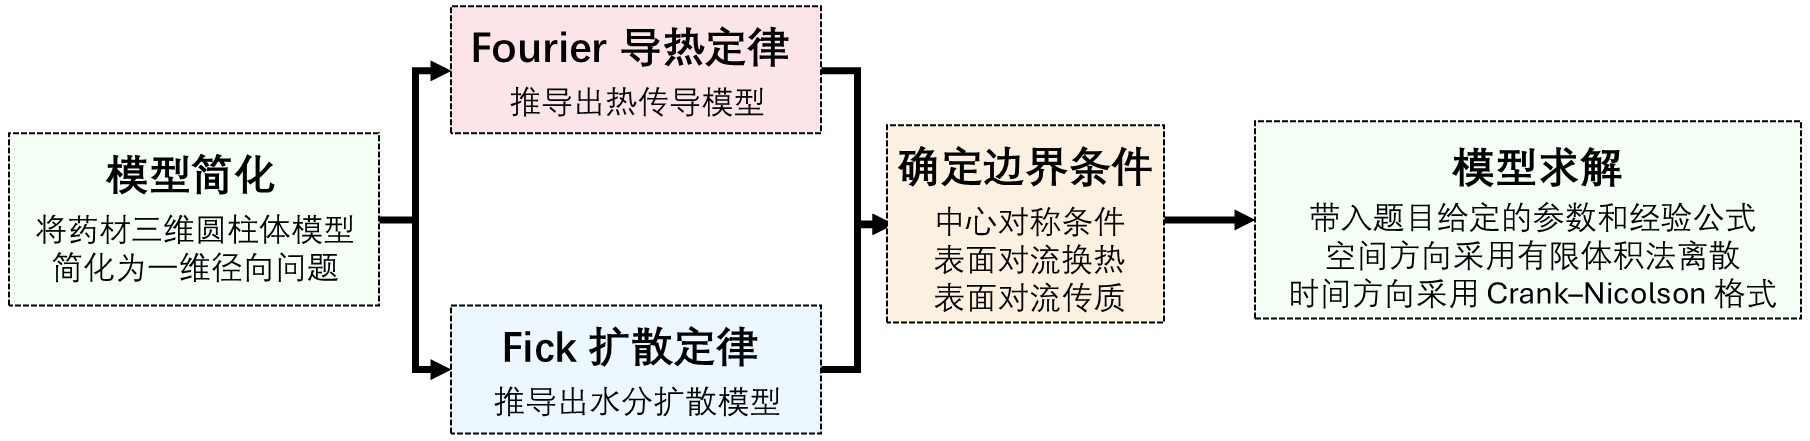
\includegraphics[width=1\textwidth]{Figures/p1_workflow.png}
    \caption{问题一传热传质模型建立与求解流程}
    \label{fig:p1_workflow}
\end{figure}


\subsubsection{模型建立}

预热平衡阶段，药材在烘房热湿环境作用下同时发生热量传递与水分迁移。考虑到药材呈近似圆柱形，且其长径比$L/R=12.5$
较大，同时题目仅要求给出距药材中心不同距离处的计算结果，因此可忽略轴向和周向的变化，将药材内部的传热传质过程简化为沿径向方向的一维径向上的问题\cite{adrover2019}。


为建立该问题的控制方程，本文采用微元分析法。图~\ref{fig:p1-mx} 展示了圆环微元分析示意图。如图所示，从圆柱形药材中沿径向取出一段半径为 \(r\)、厚度为 \(\mathrm{d}r\) 的单位长度圆环微元作为控制体。基于该微元体，后续将分别利用Fourier导热定律和Fick扩散定律，推导药材内部的温度场与水分浓度场控制方程\cite{Garcia2018}。

\begin{figure}[htbp]
    \centering
    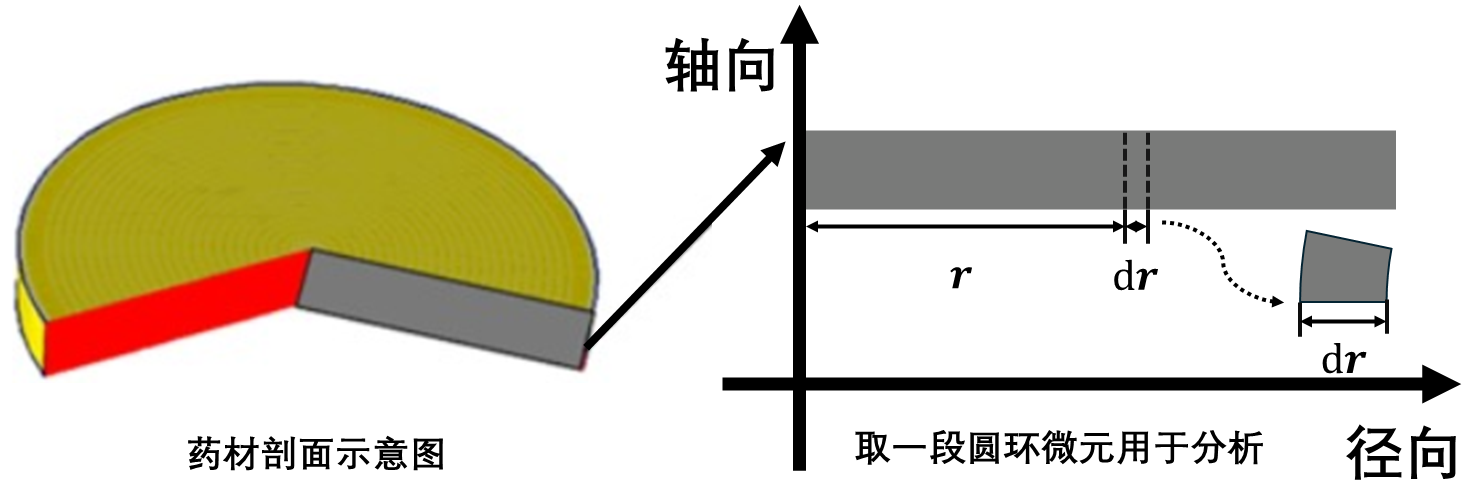
\includegraphics[width=0.80\textwidth]{Figures/p1-mx.png}
    \caption{圆环微元分析示意图}
    \label{fig:p1-mx}
\end{figure}

\paragraph{（1）温度场模型}

预热平衡阶段，药材内部热量传递以热传导为主，且因温度梯度发生传导。Fourier导热定律可以描述径向热流密度$q(r,t)$与温度梯度$\frac{\partial T}{\partial r}$的关系：
\begin{equation}
    q(r,t)=-k\frac{\partial T}{\partial r},
    \label{eq:fourier_temp}
\end{equation}
式\eqref{eq:fourier_temp}中负号表示热量由高温区向低温区传递，方向为温度的梯度的反方向。随后，沿径向取半径为 \(r\)、厚度为 \(\mathrm{d}r\) 的单位长度圆环微元。根据能量守恒，微元内能的增加量等于由导热净导入的热量。将式\eqref{eq:fourier_temp}代入该能量平衡关系，即可导出描述药材内部温度随时间和径向位置变化的控制方程：
\begin{equation}
    \rho c_p\frac{\partial T}{\partial t}
    =
    \frac{1}{r}\frac{\partial}{\partial r}
    \left(kr\frac{\partial T}{\partial r}\right).
    \label{eq:energy1}
\end{equation}
式\eqref{eq:energy1}等号左侧为热积累项，右侧为径向导热的贡献。其中$\rho$是密度，$c_p$是比热容。

\paragraph{（2）水分浓度场模型}

药材内部水分由高浓度区域向低浓度区域沿梯度反方向扩散迁移。以干基含水率 \(C\) 作为水分迁移的表征量，Fick 扩散定律可以描述这一现象，径向水分质量流密度\(J(r,t)\) 可表示为
\begin{equation}
    J(r,t)=-\rho_dD(C)\frac{\partial C}{\partial r},
    \label{eq:fick_moisture}
\end{equation}
其中 \(\rho_d\) 为干物质密度，\(D(C)\) 为水分扩散系数，负号表示水分由高浓度向低浓度方向迁移,方向依然是沿浓度梯度$\frac{\partial C}{\partial r}$的反方向。

圆环微元的水分质量守恒可以表述为微元内水分质量的变化率等于径向扩散的净流入量。同样将式\eqref{eq:fick_moisture}代入该守恒关系，而且我们可以认为预热平衡阶段 \(\rho_d\) 近似为常数，可得水分浓度控制方程
\begin{equation}
    \frac{\partial C}{\partial t}
    =
    \frac{1}{r}\frac{\partial}{\partial r}
    \left(rD(C)\frac{\partial C}{\partial r}\right).
    \label{eq:moisture1}
\end{equation}
该式\eqref{eq:energy1}等号左侧为水分浓度的时间变化，右侧为径向扩散的净贡献，其结构与温度场方程一致，但驱动势由温度梯度变为含水率梯度。

与温度场不同，水分扩散系数是由经验公式确定，可以表示为
    $D(C)=7\times10^{-9}\exp\left(-\frac{0.89}{C}\right)
    \ \mathrm{m^2/s}.
    \label{eq:diffusivity}$
且可知，\(D(C)\) 随含水率 \(C\) 的减小而显著降低，在现实中的表现为干燥后期表层含水率降低后，内部水分向表面的迁移阻力增大，干燥过程逐渐由内部扩散控制。


\paragraph{（3）边界条件}

药材几何中心处不存在优先的径向迁移方向，且根据轴对称性，所以中心处热流和水分通量均为零，即
\begin{equation}
    \left.\frac{\partial T}{\partial r}\right|_{r=0}=0,
    \qquad
    \left.\frac{\partial C}{\partial r}\right|_{r=0}=0.
    \label{eq:center_sym}
\end{equation}
式\eqref{eq:center_sym}为对称边界条件，保证了中心处温度场和水分浓度场的光滑性。

药材表面与烘房空气之间同时发生对流换热和对流传质，其物理过程如图~\ref{fig:q1_boundary} 所示。图~\ref{fig:q1_boundary}(a) 为对流换热示意图：烘房热风以对流方式将热量传给药材表面，表面热量再以导热方式向中心传递。图~\ref{fig:q1_boundary}(b) 为对流传质示意图：内部水分在含水率梯度驱动下向表面扩散，到达表面后被空气带走。

\begin{figure}[htbp]
    \centering
    \begin{subfigure}[b]{0.48\textwidth}
        \centering
        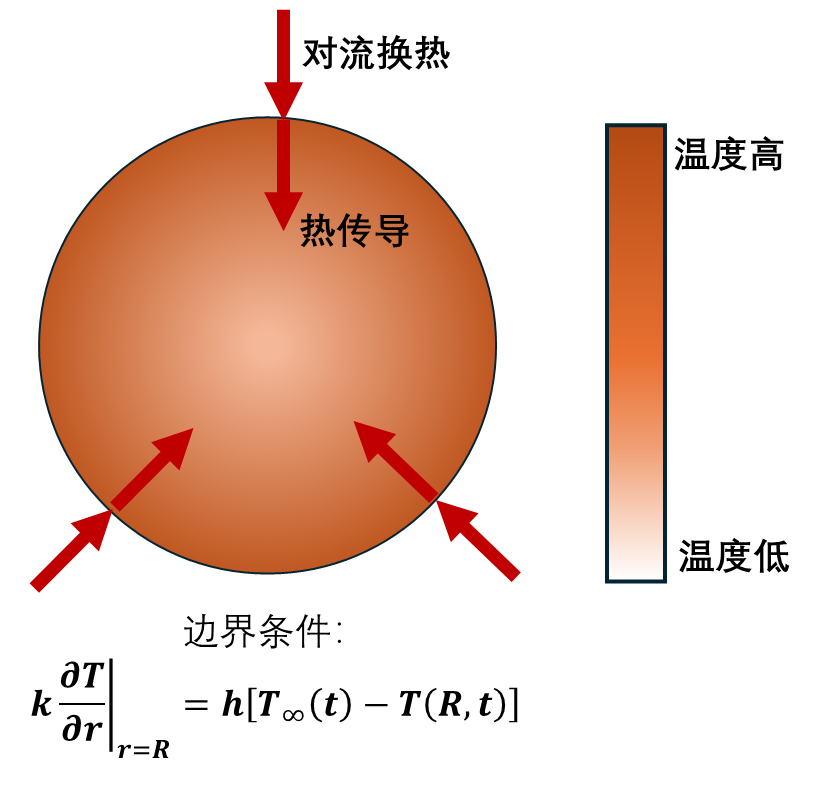
\includegraphics[width=\textwidth]{Figures/q1_heat.png}
        \caption{对流换热示意图}
        \label{fig:q1_heat}
    \end{subfigure}
    \hfill
    \begin{subfigure}[b]{0.48\textwidth}
        \centering
        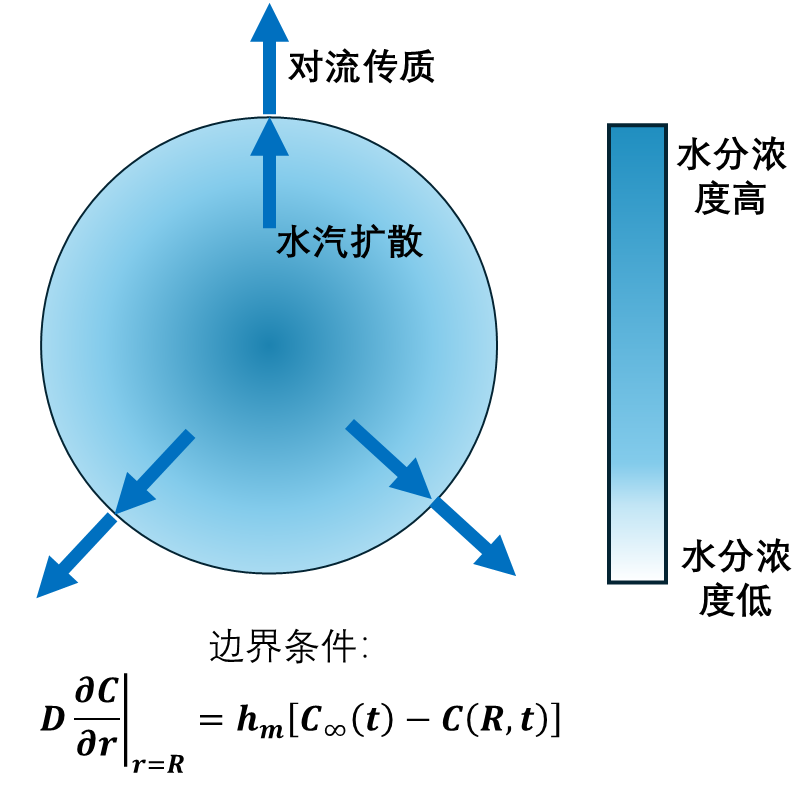
\includegraphics[width=\textwidth]{Figures/q1_mass.png}
        \caption{对流传质示意图}
        \label{fig:q1_mass}
    \end{subfigure}
    \caption{圆柱形药材横截面上的对流换热与对流传质边界条件示意图}
    \label{fig:q1_boundary}
\end{figure}

根据Newton 冷却定律，药材表面的对流换热边界条件为
\begin{equation}
    k\left.\frac{\partial T}{\partial r}\right|_{r=R}
    =
    h\left[T_\infty(t)-T(R,t)\right],
    \label{eq:conv_heat}
\end{equation}
其中$T_\infty(t)$为环境温度，对流换热系数为给定的常数 \(h=25\ \mathrm{W/(m^2\cdot K)}\)。式\eqref{eq:conv_heat}表明，药材表面由空气对流获得的热量等于其内部向外导出的热量。

类似地，药材表面的对流传质边界条件为
\begin{equation}
    D\left.\frac{\partial C}{\partial r}\right|_{r=R}
    =
    h_m\left[C_\infty(t)-C(R,t)\right],
    \label{eq:conv_mass}
\end{equation}
其中$C_\infty(t)$为环境水分含量，对流传质系数也为一个常数 \(h_m=8\times10^{-7}\ \mathrm{m/s}\)。式\eqref{eq:conv_mass}表明，内部水分扩散到表面的通量等于空气带走的水分通量。

式\eqref{eq:center_sym}、式\eqref{eq:conv_heat}和式\eqref{eq:conv_mass}与温度场方程\eqref{eq:energy1}和水分浓度场方程\eqref{eq:moisture1}一起构成封闭定解问题。

\paragraph{（4）初始条件}

烘干开始时药材内部温度和水分浓度均匀分布，因此初始条件为
$T(r,0)=28\ ^\circ\mathrm{C}=301.15\ \mathrm{K},\quad C(r,0)=2.55\ \mathrm{kg/kg},\quad 0\le r\le R.$
问题一的数学模型由控制方程与定解条件共同构成。

控制方程为
\begin{equation}
\begin{cases}
\dfrac{\partial C}{\partial t}
=\dfrac{1}{r}\dfrac{\partial}{\partial r}
\left(rD(C)\dfrac{\partial C}{\partial r}\right),\\[3mm]
\rho c_p\dfrac{\partial T}{\partial t}
=\dfrac{1}{r}\dfrac{\partial}{\partial r}
\left(kr\dfrac{\partial T}{\partial r}\right),
\end{cases}
\label{eq:model1_pde}
\end{equation}

结合中心对称条件、表面对流边界条件与初始条件
\begin{equation}
\begin{cases}
\left.\dfrac{\partial C}{\partial r}\right|_{r=0}
=\left.\dfrac{\partial T}{\partial r}\right|_{r=0}=0,\\[3mm]
D\left.\dfrac{\partial C}{\partial r}\right|_{r=R}
=h_m\left[C_\infty(t)-C(R,t)\right],\\[3mm]
k\left.\dfrac{\partial T}{\partial r}\right|_{r=R}
=h\left[T_\infty(t)-T(R,t)\right],\\[3mm]
C(r,0)=2.55,\quad
T(r,0)=301.15\ \mathrm{K},\quad
0\le r\le0.02\ \mathrm{m}.
\end{cases}
\label{eq:model1_bc}
\end{equation}

\subsubsection{模型求解}
本文根据附件1中的离散实验数据，采用单调保形三次样条插值得到连续的 \(T_\infty(t)\) 和 \(C_\infty(t)\)，从而将实际烘房环境变化直接引入模型边界条件。

上述模型同时包含径向空间变化、时间演化以及随含水率变化的非线性扩散系数，难以获得解析解，因此采用数值方法求解。在空间方向上我们采用有限体积法离散，将计算区域划分为若干控制体，通过对控制体进行守恒积分，将偏微分方程转化为满足局部守恒性的离散代数方程组\cite{LemusMondaca2013}，时间方向上采用Crank--Nicolson格式推进，在时间离散中取当前时刻与下一时刻空间离散项的平均值，在保证较高计算稳定性的同时具有二阶时间精度\cite{Ali2026}。

在空间离散方面，径向网格间距取 \(\Delta r=0.025\ \mathrm{cm}\)。题目要求的 \(0.1\ \mathrm{cm}\) 输出间隔恰为计算网格间距的整数倍，因此输出位置均落在计算节点上，无需额外插值。时间步长取 \(\Delta t=1\ \mathrm{s}\)，与题目要求的完整输出时间间隔保持一致。

在离散格式上，\(r=0\) 处根据轴对称条件采用半控制体处理，使中心节点自然满足零通量条件，可以避免虚拟节点的引入。由于 \(D(C)\) 随水分浓度变化，水分扩散方程具有非线性，因此在每个时间步内采用Picard迭代求解，利用上一次迭代得到的温度、含水率等变量更新材料物性参数，并反复求解耦合方程，直至相邻两次迭代控制在 \(10^{-8}\) 以内，以保证非线性项的收敛精度。

综上所述，具体求解流程为：首先读取附件1中的环境数据，通过单调保形三次样条插值得到连续的环境条件 \(T_\infty(t)\) 与 \(C_\infty(t)\),随后赋予药材初始温度场与水分浓度场。在每个时间步内，分别求解水分浓度场和温度场，并对非线性扩散系数进行 Picard 迭代，直至满足收敛条件。完成 \(1800\ \mathrm{s}\) 的时间推进后，按题目要求提取指定时刻与径向位置的结果，并将完整计算结果保存至 \texttt{result1.xlsx}。

\subsubsection{结果与分析}

数值求解得到预热平衡阶段药材内部温度与水分浓度的时空分布。表~\ref{tab:temp} 给出了
\(t=100,300,600,900,1200,1500,1800\ \mathrm{s}\) 时，距药材中心
\(0,0.5,1.0,1.5,2.0\ \mathrm{cm}\) 处的温度，表~\ref{tab:moist} 给出了相应位置和时刻的水分浓度。完整计算结果按照题目要求保存在 \texttt{result1.xlsx}。

\begin{table}[htbp]
\centering
\caption{30分钟内药材的温度（单位：\(^\circ\mathrm{C}\)）}
\label{tab:temp}
\begin{tabular}{cccccc}
\toprule
时间/s & \multicolumn{5}{c}{到药材中心的距离/cm} \\
\cmidrule(lr){2-6}
 & 0 & 0.5 & 1.0 & 1.5 & 2.0 \\
\midrule
100  & 28.0001 & 28.0003 & 28.0041 & 28.0327 & 28.1800 \\
300  & 28.0408 & 28.0635 & 28.1514 & 28.3680 & 28.8487 \\
600  & 28.4534 & 28.5360 & 28.8039 & 29.3159 & 30.1652 \\
900  & 29.3243 & 29.4583 & 29.8754 & 30.6161 & 31.7304 \\
1200 & 30.5427 & 30.7098 & 31.2223 & 32.1125 & 33.4276 \\
1500 & 31.9957 & 32.1867 & 32.7660 & 33.7463 & 35.1203 \\
1800 & 33.5753 & 33.7720 & 34.3642 & 35.3621 & 36.7855 \\
\bottomrule
\end{tabular}
\end{table}

\begin{table}[htbp]
\centering
\caption{30分钟内药材的水分浓度（单位：\(\mathrm{kg/kg}\)）}
\label{tab:moist}
\begin{tabular}{cccccc}
\toprule
时间/s & \multicolumn{5}{c}{到药材中心的距离/cm} \\
\cmidrule(lr){2-6}
 & 0 & 0.5 & 1.0 & 1.5 & 2.0 \\
\midrule
100  & 2.5500 & 2.5500 & 2.5500 & 2.5500 & 2.2489 \\
300  & 2.5500 & 2.5500 & 2.5500 & 2.5492 & 2.0516 \\
600  & 2.5500 & 2.5500 & 2.5500 & 2.5352 & 1.8774 \\
900  & 2.5500 & 2.5500 & 2.5497 & 2.5045 & 1.7550 \\
1200 & 2.5500 & 2.5500 & 2.5482 & 2.4646 & 1.6587 \\
1500 & 2.5500 & 2.5499 & 2.5445 & 2.4207 & 1.5788 \\
1800 & 2.5500 & 2.5497 & 2.5383 & 2.3755 & 1.5103 \\
\bottomrule
\end{tabular}
\end{table}

为更直观地展示上述数据的变化趋势，将表~\ref{tab:temp} 和表~\ref{tab:moist} 中的结果绘制成图~\ref{fig:p1-data}。



由图~\ref{fig:p1-data}(a) 可见，药材表层水分浓度下降最快，表面 \(r=2.0\ \mathrm{cm}\) 处的水分浓度持续快速下降，而中心 \(r=0\sim1.0\ \mathrm{cm}\) 区域在整个 \(1800\ \mathrm{s}\) 内几乎保持初始值，内外出现了明显的区别，这说明了水分迁移的过程中，失水首先发生在表层，并随时间的推移缓慢向内推进，干燥锋面在 \(1800\ \mathrm{s}\) 内尚未到达 \(r=1.0\ \mathrm{cm}\) 以内区域。

由图~\ref{fig:p1-data}(b) 可见，各径向位置的温度均随时间升高，但速度同样存在明显差异：表面 \(r=2.0\ \mathrm{cm}\) 处升温最快，中心 \(r=0\) 处最慢，二者温差随时间持续拉大。从传热机理上看这是因为环境的热量首先以对流方式传给药材表面，再依靠径向热传递逐渐向内部传递，越靠近表面，温度对环境的响应越迅速。

\begin{figure}[htbp]
  \centering
  \begin{subfigure}[b]{0.48\textwidth}
    \centering
    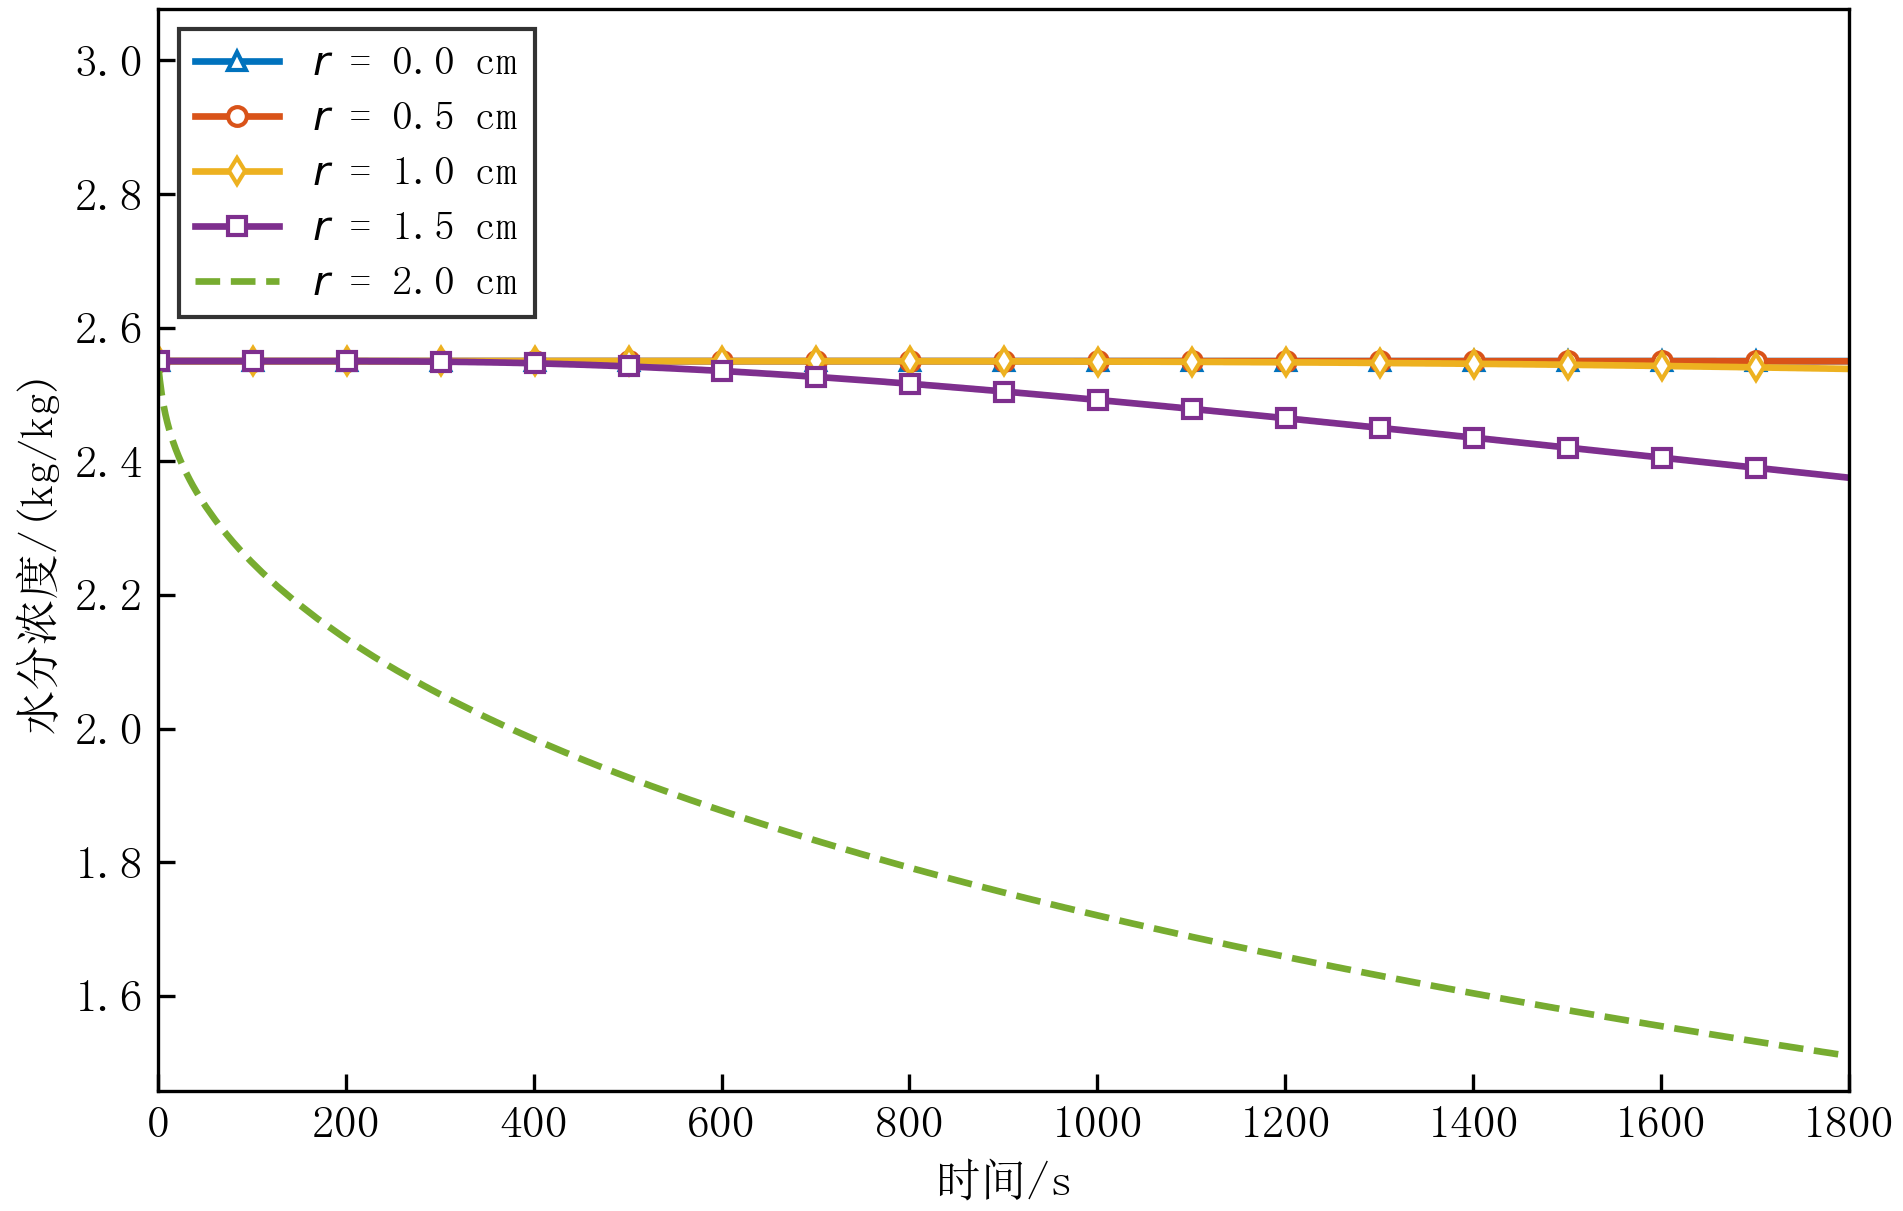
\includegraphics[width=\textwidth]{Figures/p1-C.png}
    \caption{预热平衡阶段药材水分浓度随时间变化}
    \label{fig:p1-c}
  \end{subfigure}
  \hfill
  \begin{subfigure}[b]{0.48\textwidth}
    \centering
    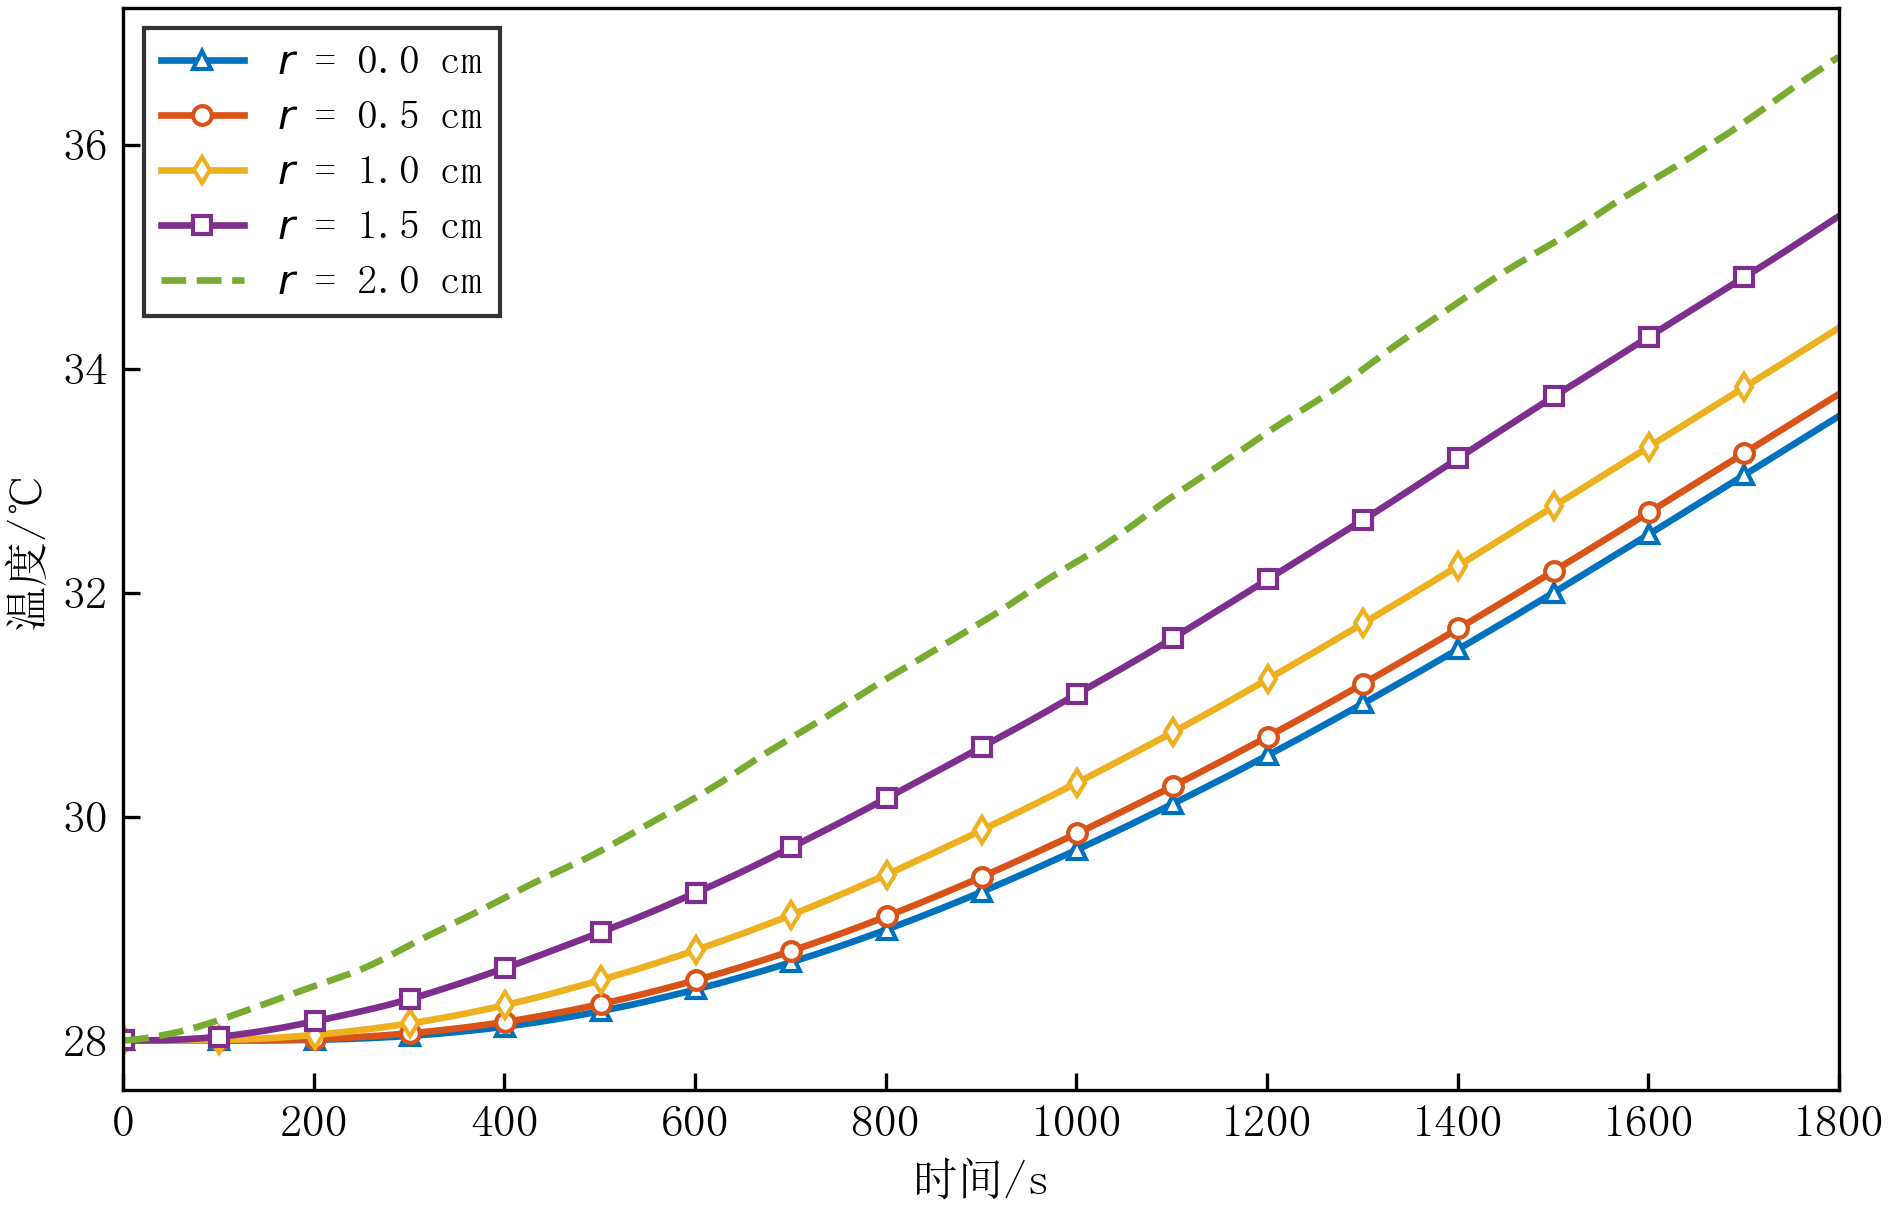
\includegraphics[width=\textwidth]{Figures/p1-T.png}
    \caption{预热平衡阶段药材温度随时间变化}
    \label{fig:p1-T}
  \end{subfigure}
  \caption{预热平衡阶段药材水分浓度与温度随时间变化}
  \label{fig:p1-data}
\end{figure}

对比温度场与水分浓度场可以发现，温度扰动在 \(1800\ \mathrm{s}\) 内已经深入药材内部，而水分扰动主要局限于表层。这一差异的根本原因在于热扩散率约为 \(1.69\times10^{-7}\ \mathrm{m^2/s}\)，而初始水分扩散系数仅约 \(4.94\times10^{-9}\ \mathrm{m^2/s}\)，二者相差约两个数量级。这也表明，后续恒温干燥阶段的烘干时间将主要由水分在药材内部的扩散过程控制，而非由热量传递控制。



\subsubsection{模型检验与灵敏度分析}

在得到预热平衡阶段温度场与水分浓度场的数值解后，为了检验模型和结果的可靠性，本文将先进行守恒性与收敛性检验，再对关键参数进行灵敏度分析。

\paragraph{（1）数值可靠性检验}

为验证数值格式的可靠性，本文从守恒性、时间步无关性和空间网格无关性三方面进行检验，结果如表~\ref{tab:verification} 所示。

\begin{table}[htbp]
\centering
\caption{数值可靠性检验结果}
\label{tab:verification}
\renewcommand{\arraystretch}{1.15}
\begin{tabular}{lc}
\toprule
检验项 & 数值 \\
\midrule
水分守恒残差 & \(3.4\times10^{-15}\) \\
能量守恒残差 & \(3.1\times10^{-13}\) \\
时间步长减半前后温度差 & \(7.1\times10^{-6}\) \\
空间网格减半前后温度差 & \(1.5\times10^{-4}\) \\
\bottomrule
\end{tabular}
\end{table}

由表~\ref{tab:verification} 可见，水分与能量守恒残差均在 \(10^{-13}\) 量级，时间步长与空间网格减半后温度变化均不超过 \(1.5\times10^{-4}\)，远小于题目要求的四位小数精度 \(10^{-4}\)。

\paragraph{（2）参数灵敏度分析}

在确认数值可靠性后，进一步评估各参数与假设对温度场的影响。以 \(t=1800\,\mathrm{s}\) 时药材中心温度 \(T(0,1800\,\mathrm{s})=33.575\,^\circ\mathrm{C}\) 为基准，对各因素进行扰动分析，结果如表~\ref{tab:sens_q1} 所示。

\begin{table}[htbp]
\centering
\caption{问题一灵敏度分析}
\label{tab:sens_q1}
\renewcommand{\arraystretch}{1.15}
\begin{tabular}{lcc}
\toprule
扰动因素 & 温度变化 \(\Delta T\) & 相对基准 \\
\midrule
汽化潜热项（关 \(\to\) 开） & \(27.62\ \mathrm{K}\) & \(82.3\%\) \\
比热容 \(c_p\) 扰动 \(\pm 10\%\) & \(0.525\ \mathrm{K}\) & \(1.56\%\) \\
对流换热系数 \(h\) 扰动 \(\pm 10\%\) & \(0.278\ \mathrm{K}\) & \(0.83\%\) \\
热传导系数 \(k\) 扰动 \(\pm 10\%\) & \(0.255\ \mathrm{K}\) & \(0.76\%\) \\
网格与时间步加密 & \(1.5\times10^{-4}\ \mathrm{K}\) & \(4\times10^{-6}\) \\
\bottomrule
\end{tabular}
\end{table}

由表~\ref{tab:sens_q1} 可见，各因素对温度场的影响呈明显的量级分层，可分为三个层次。

\textbf{第一层为汽化潜热项}，其影响远大于其余所有因素之和。当汽化潜热项由关闭改为开启时，中心温度变化达 \(27.62\,\mathrm{K}\)，相对基准偏差为 \(82.3\%\)，远大于其他所有因素之和。这说明是否计入汽化潜热是问题一唯一需要专门论证的关键假设。我们认为：由于附录未给出汽化潜热 \(L_v\)，且若按给定的 \(h_m=8\times10^{-7}\,\mathrm{m/s}\) 直接引入潜热汇，模型会给出 \(t=1800\,\mathrm{s}\) 时中心温度约为 \(5.95\,^\circ\mathrm{C}\)，低于该空气约 \(25\,^\circ\mathrm{C}\) 的湿球温度，属于非物理结果。因此正文模型中都不再不计汽化潜热，并在模型假设中予以说明。

\textbf{第二层为传热参数}，包括比热容 \(c_p\)、对流换热系数 \(h\) 和热传导系数 \(k\)。在 \(\pm 10\%\) 扰动下，三者引起的温度变化分别为 \(0.525\,\mathrm{K}\)、\(0.278\,\mathrm{K}\) 和 \(0.255\,\mathrm{K}\)，相对基准均在 \(1.6\%\) 以内。这说明模型对传热参数的敏感性处于可控范围。

\textbf{第三层为水分参数与离散参数}。水分扩散系数 \(D_0\) 与对流传质系数 \(h_m\) 对温度场完全无影响（变化量为 0），网格与时间步加密对温度的影响也仅为 \(4\times10^{-6}\)。我们的模型对这些参数完全不敏感。

综合以上分析，我们的模型具有良好鲁棒性，结果也在合理的范围之内。













\subsection{问题二：Fick–Fourier 热–湿双向耦合模型}

问题二要求将问题一的模型推广至整个烘干过程。首先我们分析附件 1 中的数据，确定预热平衡和恒温干燥两个阶段的分界点。
之后与问题一类似，沿用一维轴对称假设，由Fick 定律和 Fourier 定律分别建立水分与温度方程，接着同样确定三个边界条件。
最后带入题目给定的参数和经验公式，得到问题二中热--湿双向耦合模型。
为了求解，在问题一求解方法的基础之上，为了求解双向耦合函数，我们还加入了Picard 迭代,利用上一次迭代的数据更新函数反复求解耦合方程直到收敛，这样我们就求解出整个烘干过程中温度和水分含量的时空关系。
图~\ref{fig:p2_workflow} 给出了建模和求解思路。
\begin{figure}[htbp]
    \centering
    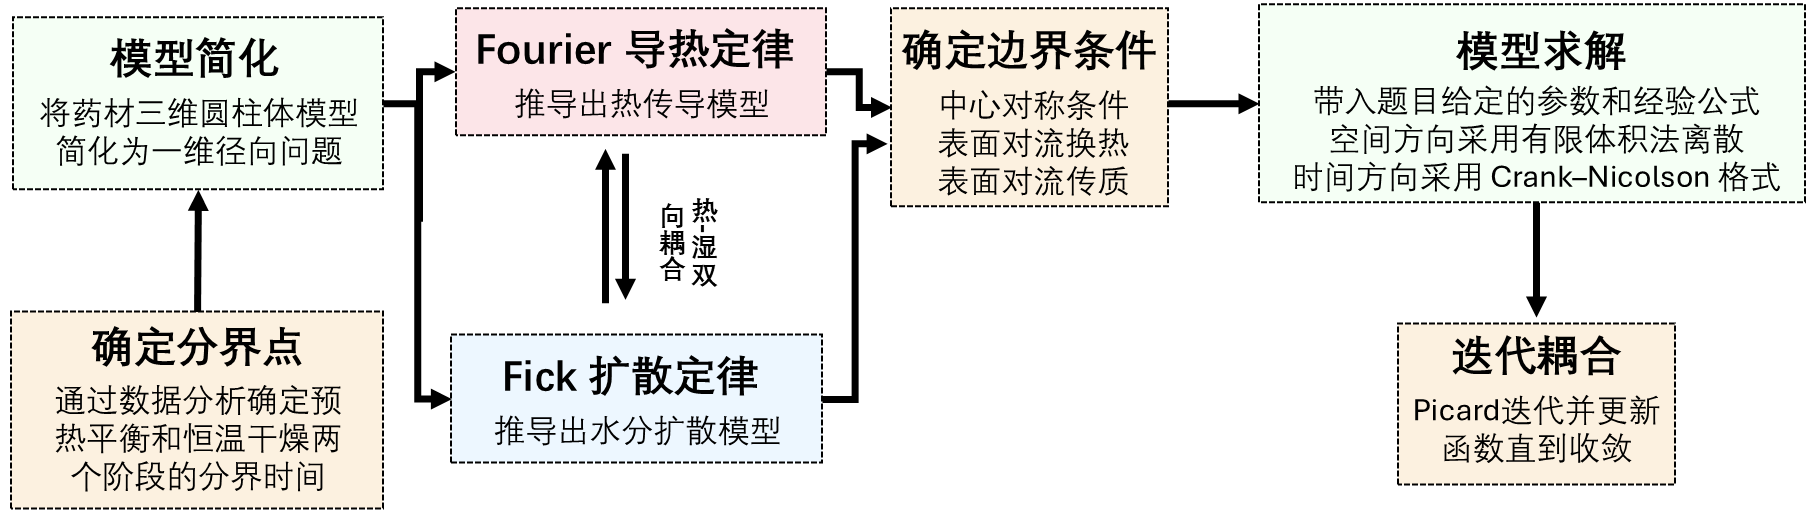
\includegraphics[width=0.8\textwidth]{Figures/p2_workflow.png}
    \caption{问题二全过程传热传质模型建立与求解流程}
    \label{fig:p2_workflow}
\end{figure}


\subsubsection{两阶段划分与环境条件}

首先需要确定两个阶段的分界时刻，并据此给出整个烘干过程中的烘房环境条件。

根据问题一建立的模型，将计算时间延长至 $4\,\mathrm{h}$，并以药材与烘房之间的温度平衡程度作为阶段转换的主要判据。计算结果表明，烘房温度约在 $1.43\,\mathrm{h}$ 后进入稳定平台，而药材内部由于径向传热存在一定滞后。当药材中心温度与烘房温度之差首次小于 $1\,\mathrm{K}$ 时，对应时刻约为 $1.94\,\mathrm{h}$。上述过程如图 \ref{fig:stage-division} 所示。图~\ref{fig:p2_workflow} 给出了建模和求解的思路。

\begin{figure}[htbp]
  \centering
  \begin{subfigure}[b]{0.48\textwidth}
    \centering
    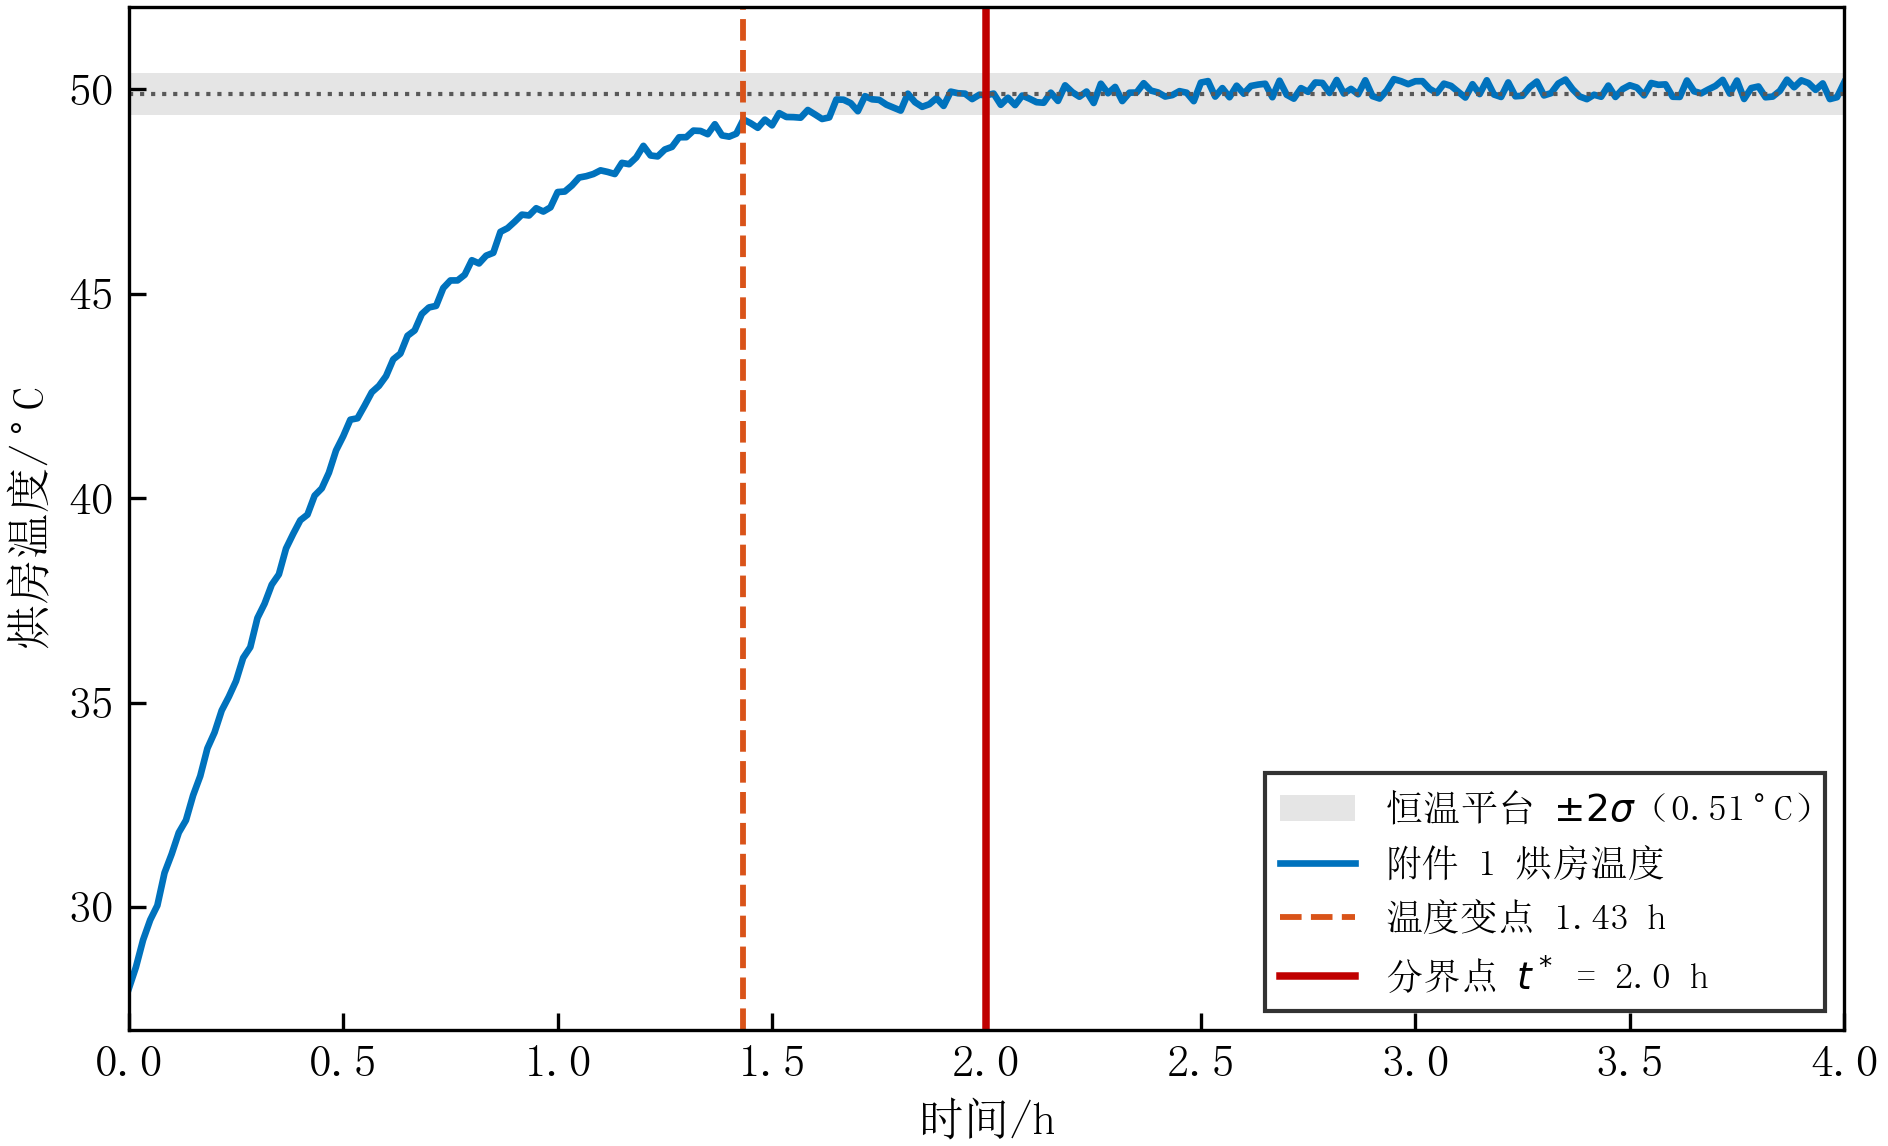
\includegraphics[width=\textwidth]{Figures/p2-env.png}
    \caption{烘房温度变化曲线}
    \label{fig:p2-env}
  \end{subfigure}
  \hfill
  \begin{subfigure}[b]{0.48\textwidth}
    \centering
    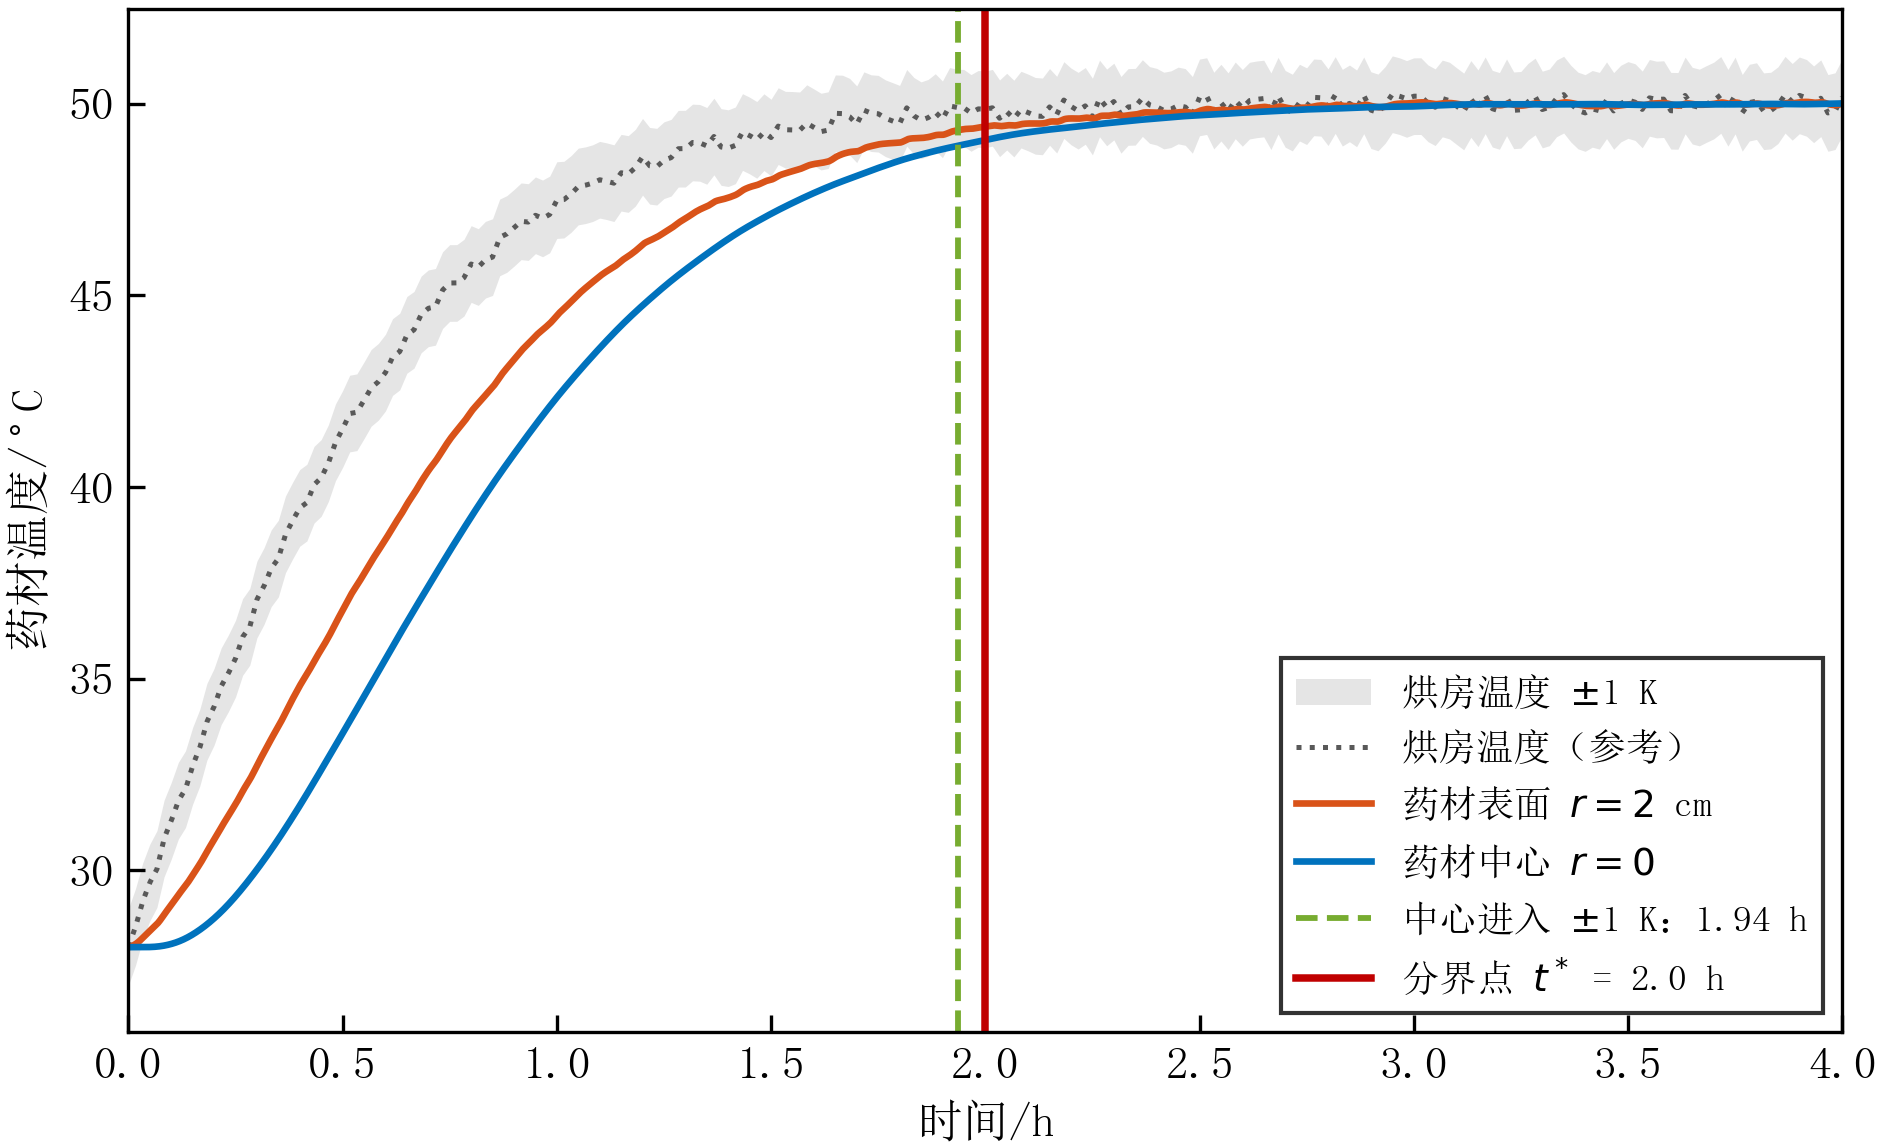
\includegraphics[width=\textwidth]{Figures/p2-in.png}
    \caption{药材内部温度变化曲线}
    \label{fig:p2-in}
  \end{subfigure}
  \caption{两阶段分界点的确定}
  \label{fig:stage-division}
\end{figure}

由图 \ref{fig:stage-division}(a) 可见，烘房温度在 $1.43\,\mathrm{h}$ 后进入恒温平台，平台温度约为 $50.0\,^\circ\mathrm{C}$；由图 \ref{fig:stage-division}(b) 可见，药材中心温度直至 $1.94\,\mathrm{h}$ 才进入烘房温度 $\pm 1\,\mathrm{K}$ 的灰带内，表明此时药材内部才基本达到热平衡。综合考虑药材内部的热平衡程度以及烘房环境的稳定性，本文取
$t^*=7200\,\mathrm{s}=2.0\,\mathrm{h}$
作为预热平衡阶段与恒温干燥阶段的分界时刻。

在 $0\leq t\leq t^*$ 内，烘房温度和水分浓度均由附件1中的离散数据进行线性插值得到；当 $t>t^*$ 时，烘房环境视为恒定。根据附件1数据，稳定阶段烘房温度和水分浓度分别取 $50.0\,^\circ\mathrm{C}$ 和 $0.050\,\mathrm{kg/kg}$。

因此，整个烘干过程中的环境温度和水分浓度可表示为

\begin{equation}
T_\infty(t)=
\begin{cases}
T_{\mathrm{air}}(t), & 0\leq t\leq t^*,\\
50.0\,^\circ\mathrm{C}, & t>t^*,
\label{eq:T}
\end{cases}
\end{equation}
\begin{equation}
C_\infty(t)=
\begin{cases}
C_{\mathrm{air}}(t), & 0\leq t\leq t^*,\\
0.050\,\mathrm{kg/kg}, & t>t^*,
\end{cases}
\label{eq:C}
\end{equation}
其中$T_{\mathrm{air}}(t)$ 和 $C_{\mathrm{air}}(t)$分别表示由附件1离散数据插值得到的温度和水分浓度函数。




\subsubsection{控制方程}

按照问题一中的假设，药材仍视为轴对称圆柱，仅考虑径向方向的传热与传质。

以干基水分浓度 $C$ 为驱动势，根据 Fick 定律，水分质量通量$J$可表示为
\begin{equation}
J=-\rho_d D(C,T)\frac{\partial C}{\partial r},
\end{equation}
其中，$\rho_d$ 为干物质密度。由水分质量守恒，并将 $\rho_d$ 视为常数，可得水分扩散方程
\begin{equation}
\frac{\partial C}{\partial t}
=
\frac{1}{r}
\frac{\partial}{\partial r}
\left(
rD(C,T)\frac{\partial C}{\partial r}
\right).
\label{eq:moisture2}
\end{equation}

同理根据 Fourier 导热定律
\begin{equation}
q=-k(C)\frac{\partial T}{\partial r},
\end{equation}
对圆柱微元进行能量守恒，可得药材内部温度控制方程
\begin{equation}
\rho(C)c_p(C)\frac{\partial T}{\partial t}
=
\frac{1}{r}
\frac{\partial}{\partial r}
\left(
k(C)r\frac{\partial T}{\partial r}
\right).
\label{eq:energy2}
\end{equation}

由式 \eqref{eq:moisture2} \eqref{eq:energy2} 可知，问题二中的传热传质过程存在双向耦合关系。水分浓度$C$的变化会引起$\rho(C)$、$c_p(C)$和$k(C)$的变化影响药材内部的温度场，反过来水分扩散系数 $D(C,T)$ 同时受到温度和水分浓度的影响，使温度变化进一步影响水分迁移过程。

\subsubsection{物性参数}

根据附录3，药材密度、比热容和热传导系数不再是一个常数，分别为
$$
\rho(C)=650+128C,
\quad
c_p(C)=1450+2736\frac{C}{C+1},
\quad
k(C)=0.21+0.38\frac{C}{C+1}.
$$
水分扩散系数表示为
$$
D(C,T)
=
2.4\times10^{-3}
\exp\left(-\frac{0.45}{C}\right)
\exp\left(-\frac{3850}{T}\right),
\label{eq:D2}
$$
其中 $T$ 必须采用绝对温度 $\mathrm{K}$。

\subsubsection{定解条件}
问题二的定界条件与问题一中的相同。
在药材中心 $r=0$ 处，由轴对称性可得
\begin{equation}
\left.
\frac{\partial C}{\partial r}
\right|_{r=0}
=
0,
\qquad
\left.
\frac{\partial T}{\partial r}
\right|_{r=0}
=
0.
\end{equation}

在药材表面 $r=R$ 处，采用对流传质和对流换热边界条件
\begin{equation}
D(C,T)
\left.
\frac{\partial C}{\partial r}
\right|_{r=R}
=
h_m
\left[
C_\infty(t)-C(R,t)
\right],
\end{equation}
\begin{equation}
k(C)
\left.
\frac{\partial T}{\partial r}
\right|_{r=R}
=
h
\left[
T_\infty(t)-T(R,t)
\right],
\end{equation}
其中
$h=25\,\mathrm{W/(m^2\cdot K)},
\quad
h_m=8\times10^{-7}\,\mathrm{m/s}.$

全过程的初始状态为
$C(r,0)=2.55\,\mathrm{kg/kg},
\quad
T(r,0)=28\,^\circ\mathrm{C}=301.15\,\mathrm{K},
\quad
0\leq r\leq0.02\,\mathrm{m}.$，与问题一一致。


综上，问题二的全过程传热传质模型由控制方程与定解条件共同构成。

控制方程为
\begin{equation}
\begin{cases}
\dfrac{\partial C}{\partial t}
=
\dfrac{1}{r}\dfrac{\partial}{\partial r}
\left(rD(C,T)\dfrac{\partial C}{\partial r}\right),\\[3mm]
\rho(C)c_p(C)\dfrac{\partial T}{\partial t}
=
\dfrac{1}{r}\dfrac{\partial}{\partial r}
\left(k(C)\,r\dfrac{\partial T}{\partial r}\right),
\end{cases}
\label{eq:model2_pde}
\end{equation}
其中水分扩散系数 \(D(C,T)\) 与物性参数 \(\rho(C)\)、\(c_p(C)\)、\(k(C)\) 均由附录3经验公式给出。

结合中心对称条件、表面对流边界条件与初始条件
\begin{equation}
\begin{cases}
\left.\dfrac{\partial C}{\partial r}\right|_{r=0}
=\left.\dfrac{\partial T}{\partial r}\right|_{r=0}=0,\\[3mm]
D(C,T)\left.\dfrac{\partial C}{\partial r}\right|_{r=R}
=h_m\left[C_\infty(t)-C(R,t)\right],\\[3mm]
k(C)\left.\dfrac{\partial T}{\partial r}\right|_{r=R}
=h\left[T_\infty(t)-T(R,t)\right],\\[3mm]
C(r,0)=2.55\,\mathrm{kg/kg},\quad
T(r,0)=301.15\,\mathrm{K},\quad
0\le r\le0.02\,\mathrm{m},
\end{cases}
\label{eq:model2_bc}
\end{equation}
即构成封闭的定解问题。其中环境条件 \(T_\infty(t)\)、\(C_\infty(t)\) 的表达式由式 \eqref{eq:T}和式 \eqref{eq:C}给出。

我们将求得的温度和水分浓度随时间和径向位置变化的函数记为 $T(r,t)$ 和 $C(r,t)$ ，在后续问题中方便参与求解。

\subsubsection{模型求解}

由于式 \eqref{eq:model2_bc} 中的 $D(C,T)$、$k(C)$、$\rho(C)$ 和 $c_p(C)$ 均随药材状态变化，所建立的模型属于非线性耦合偏微分方程组。本文采用有限体积法进行空间离散，并采用 Crank--Nicolson 格式进行时间推进。

在径向方向将 $0\leq r\leq0.02\,\mathrm{m}$ 均匀划分，内部计算网格取
$\Delta r=0.025\,\mathrm{cm}
=2.5\times10^{-4}\,\mathrm{m},$
即将药材半径方向划分为 $80$ 个空间区间。题目要求的 $0.1\,\mathrm{cm}$ 输出间隔为计算网格的整数倍，因此计算结果可以直接提取，无需进行额外空间插值。

时间步长取$\Delta t=1\,\mathrm{s}$,计算时间覆盖题目要求的前 $3\,\mathrm{h}$，即 $1800s$。

对于每一个时间步，根据当前迭代得到的 $C$ 和 $T$，计算各控制体内的物性参数
$$\rho(C),\qquad
c_p(C),\qquad
k(C),\qquad
D(C,T).$$


随后分别对水分扩散方程和温度方程进行离散求解，并通过 Picard 迭代不断更新物性参数，使温度场与水分浓度场达到自洽。

具体而言，在第 $n+1$ 个时间层内，以第 $m$ 次迭代结果 $C^{(m)},\qquad T^{(m)}$计算
$$D^{(m)}
=
D\left(C^{(m)},T^{(m)}\right),
\quad
k^{(m)}
=
k\left(C^{(m)}\right),$$
以及
$$\left(\rho c_p\right)^{(m)}
=
\rho\left(C^{(m)}\right)
c_p\left(C^{(m)}\right).$$
在此基础上求得新的 $C^{(m+1)}$ 和 $T^{(m+1)}$，并不断重复上述过程，直至满足
\begin{equation}
\max_i\left|C_i^{(m+1)}-C_i^{(m)}\right|
<10^{-10},
\qquad
\max_i\left|T_i^{(m+1)}-T_i^{(m)}\right|
<10^{-10}.
\end{equation}
数值计算表明，通常经过 $2\sim3$ 次迭代即可达到收敛要求。

在空间离散过程中，内部控制体采用守恒形式进行离散；各控制体界面的 $D$ 和 $k$ 均采用调和平均，以降低物性参数空间变化对数值计算的影响。中心节点采用半控制体处理，自然满足 $r=0$ 处的零通量条件；表面节点采用半控制体结合对流边界条件进行离散。

模型计算过程中，$T_\infty(t)$ 和 $C_\infty(t)$ 都是以 $t=7200s$ 为分界的分段函数，其表达式分别由式 \eqref{eq:T}和式 \eqref{eq:C} 给出。

\newpage

\subsubsection{计算结果}

根据上述模型进行数值求解，得到药材在前 \(3\,\mathrm{h}\) 内的温度场及水分浓度场变化结果。表~\ref{tab:problem2-temperature} 和表~\ref{tab:problem2-moisture} 分别给出了每隔 \(0.5\,\mathrm{h}\)、到药材中心距离为 \(0,0.5,1,1.5,2\,\mathrm{cm}\) 处的温度和水分浓度。

\begin{table}[htbp]
\centering
\caption{3小时内药材的温度（单位：\(^\circ\mathrm{C}\)）}
\label{tab:problem2-temperature}
\renewcommand{\arraystretch}{1.15}
\begin{tabular}{cccccc}
\toprule
\multirow{2}{*}{时间/h} & \multicolumn{5}{c}{到药材中心的距离/cm} \\
\cmidrule(lr){2-6}
 & 0 & 0.5 & 1 & 1.5 & 2 \\
\midrule
0.5 & 32.1893 & 32.3822 & 32.9660 & 33.9608 & 35.4131 \\
1.0 & 40.3817 & 40.5537 & 41.0606 & 41.8783 & 42.9977 \\
1.5 & 45.8468 & 45.9349 & 46.1930 & 46.6052 & 47.1402 \\
2.0 & 48.4503 & 48.4881 & 48.5985 & 48.7736 & 49.0033 \\
2.5 & 49.5468 & 49.5595 & 49.5965 & 49.6546 & 49.7298 \\
3.0 & 49.8770 & 49.8805 & 49.8907 & 49.9066 & 49.9273 \\
\bottomrule
\end{tabular}
\end{table}

\begin{table}[htbp]
\centering
\caption{3小时内药材的水分浓度（单位：\(\mathrm{kg/kg}\)）}
\label{tab:problem2-moisture}
\renewcommand{\arraystretch}{1.15}
\begin{tabular}{cccccc}
\toprule
\multirow{2}{*}{时间/h} & \multicolumn{5}{c}{到药材中心的距离/cm} \\
\cmidrule(lr){2-6}
 & 0 & 0.5 & 1 & 1.5 & 2 \\
\midrule
0.5 & 2.5499 & 2.5489 & 2.5255 & 2.3258 & 1.6486 \\
1.0 & 2.5257 & 2.4947 & 2.3578 & 2.0230 & 1.4711 \\
1.5 & 2.3860 & 2.3256 & 2.1344 & 1.8020 & 1.3475 \\
2.0 & 2.1708 & 2.1084 & 1.9236 & 1.6259 & 1.2311 \\
2.5 & 1.9561 & 1.9001 & 1.7356 & 1.4719 & 1.1174 \\
3.0 & 1.7655 & 1.7159 & 1.5699 & 1.3333 & 1.0083 \\
\bottomrule
\end{tabular}
\end{table}

为更直观地展示前 \(3\,\mathrm{h}\) 内温度场与水分浓度场的变化趋势，将上述结果绘制成图~\ref{fig:q2-data}。



由图~\ref{fig:q2-data}(a) 可见，各径向位置的温度均随时间升高，但响应速度存在显著差异。表面 \(r=2.0\,\mathrm{cm}\) 处升温最快，在约 \(1.5\,\mathrm{h}\) 时已接近 \(50\,^\circ\mathrm{C}\) 的烘房平台温度；中心 \(r=0\) 处升温最慢，存在明显的滞后。约 \(2.0\,\mathrm{h}\) 后，各径向位置温度曲线趋于重合，表明药材内部已基本达到热平衡。这与表~\ref{tab:problem2-temperature} 中的数据体现的结果一致。

\begin{figure}[htbp]
    \centering
    \begin{subfigure}[b]{0.48\textwidth}
        \centering
        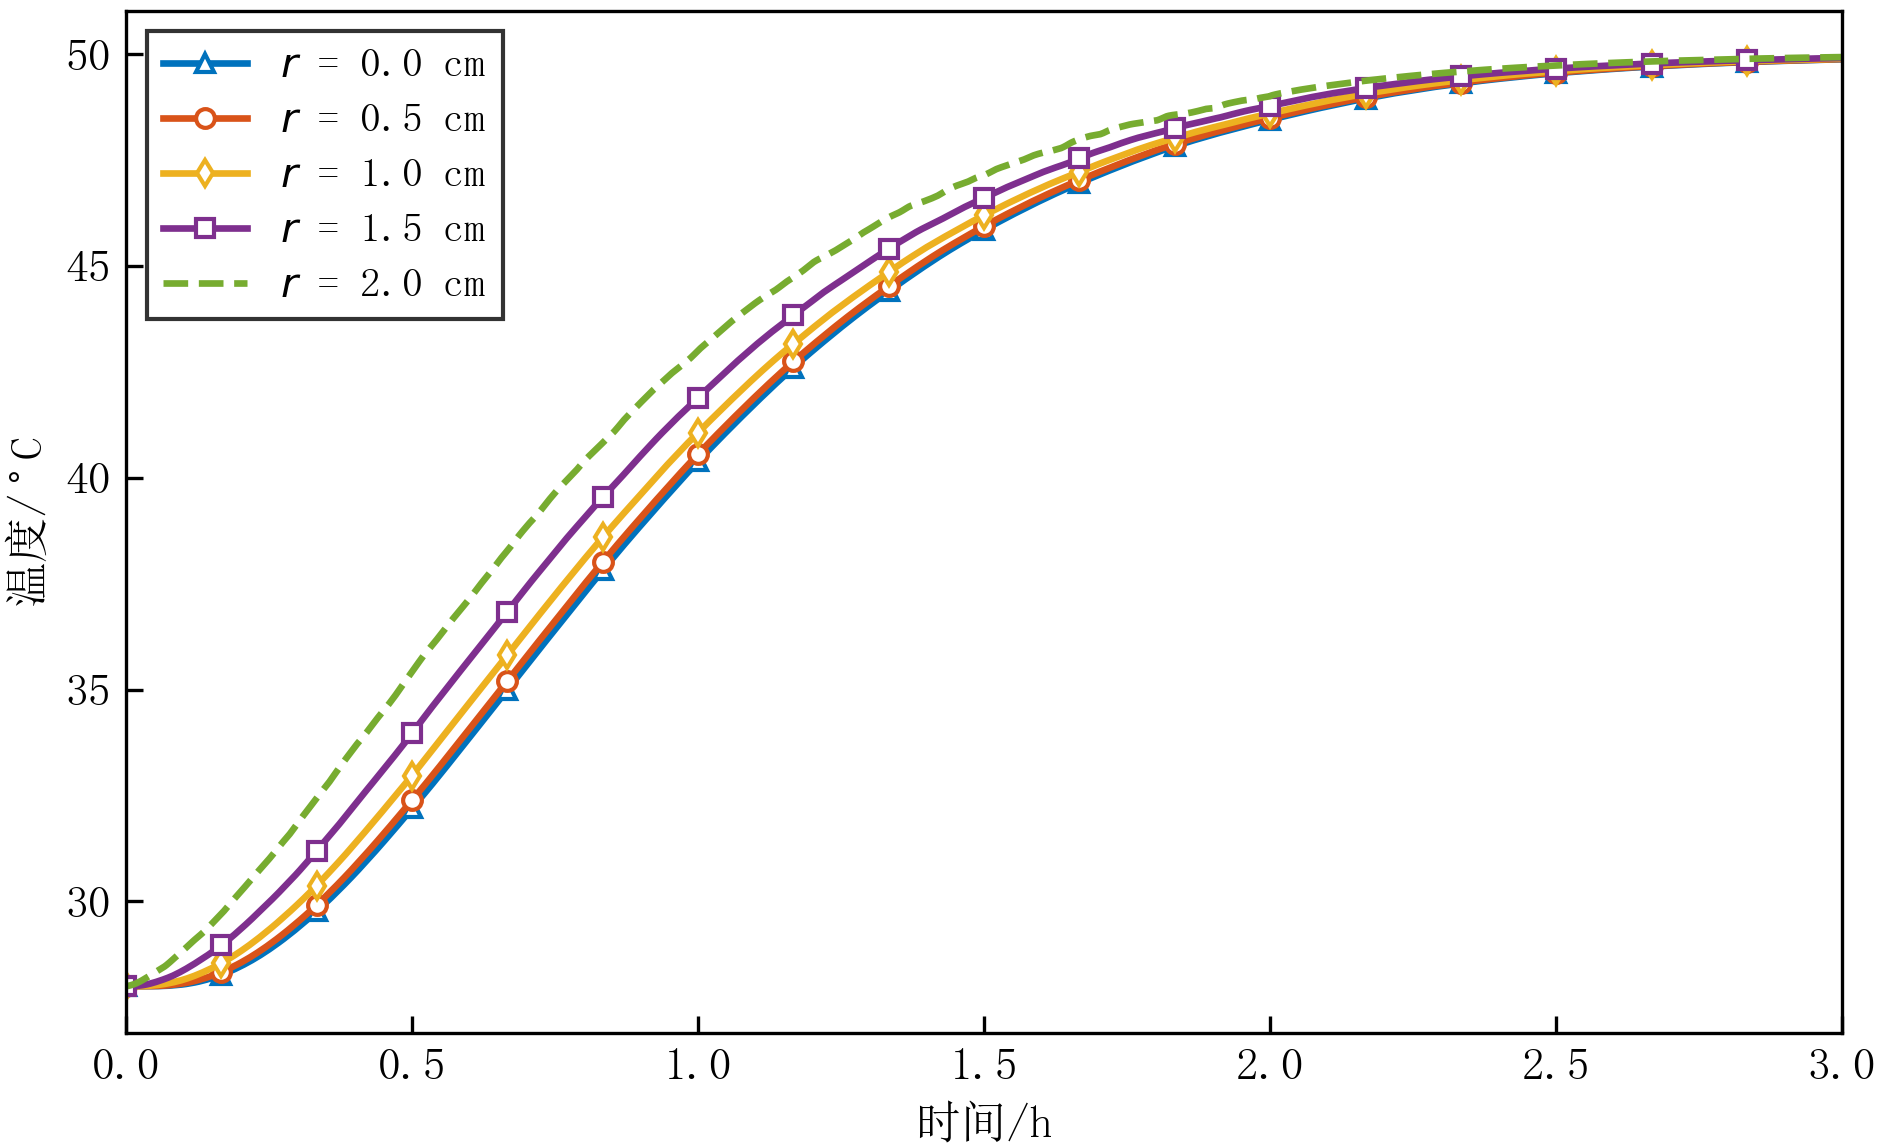
\includegraphics[width=\textwidth]{Figures/q2-T.png}
        \caption{温度随时间变化}
        \label{fig:q2-T}
    \end{subfigure}
    \hfill
    \begin{subfigure}[b]{0.48\textwidth}
        \centering
        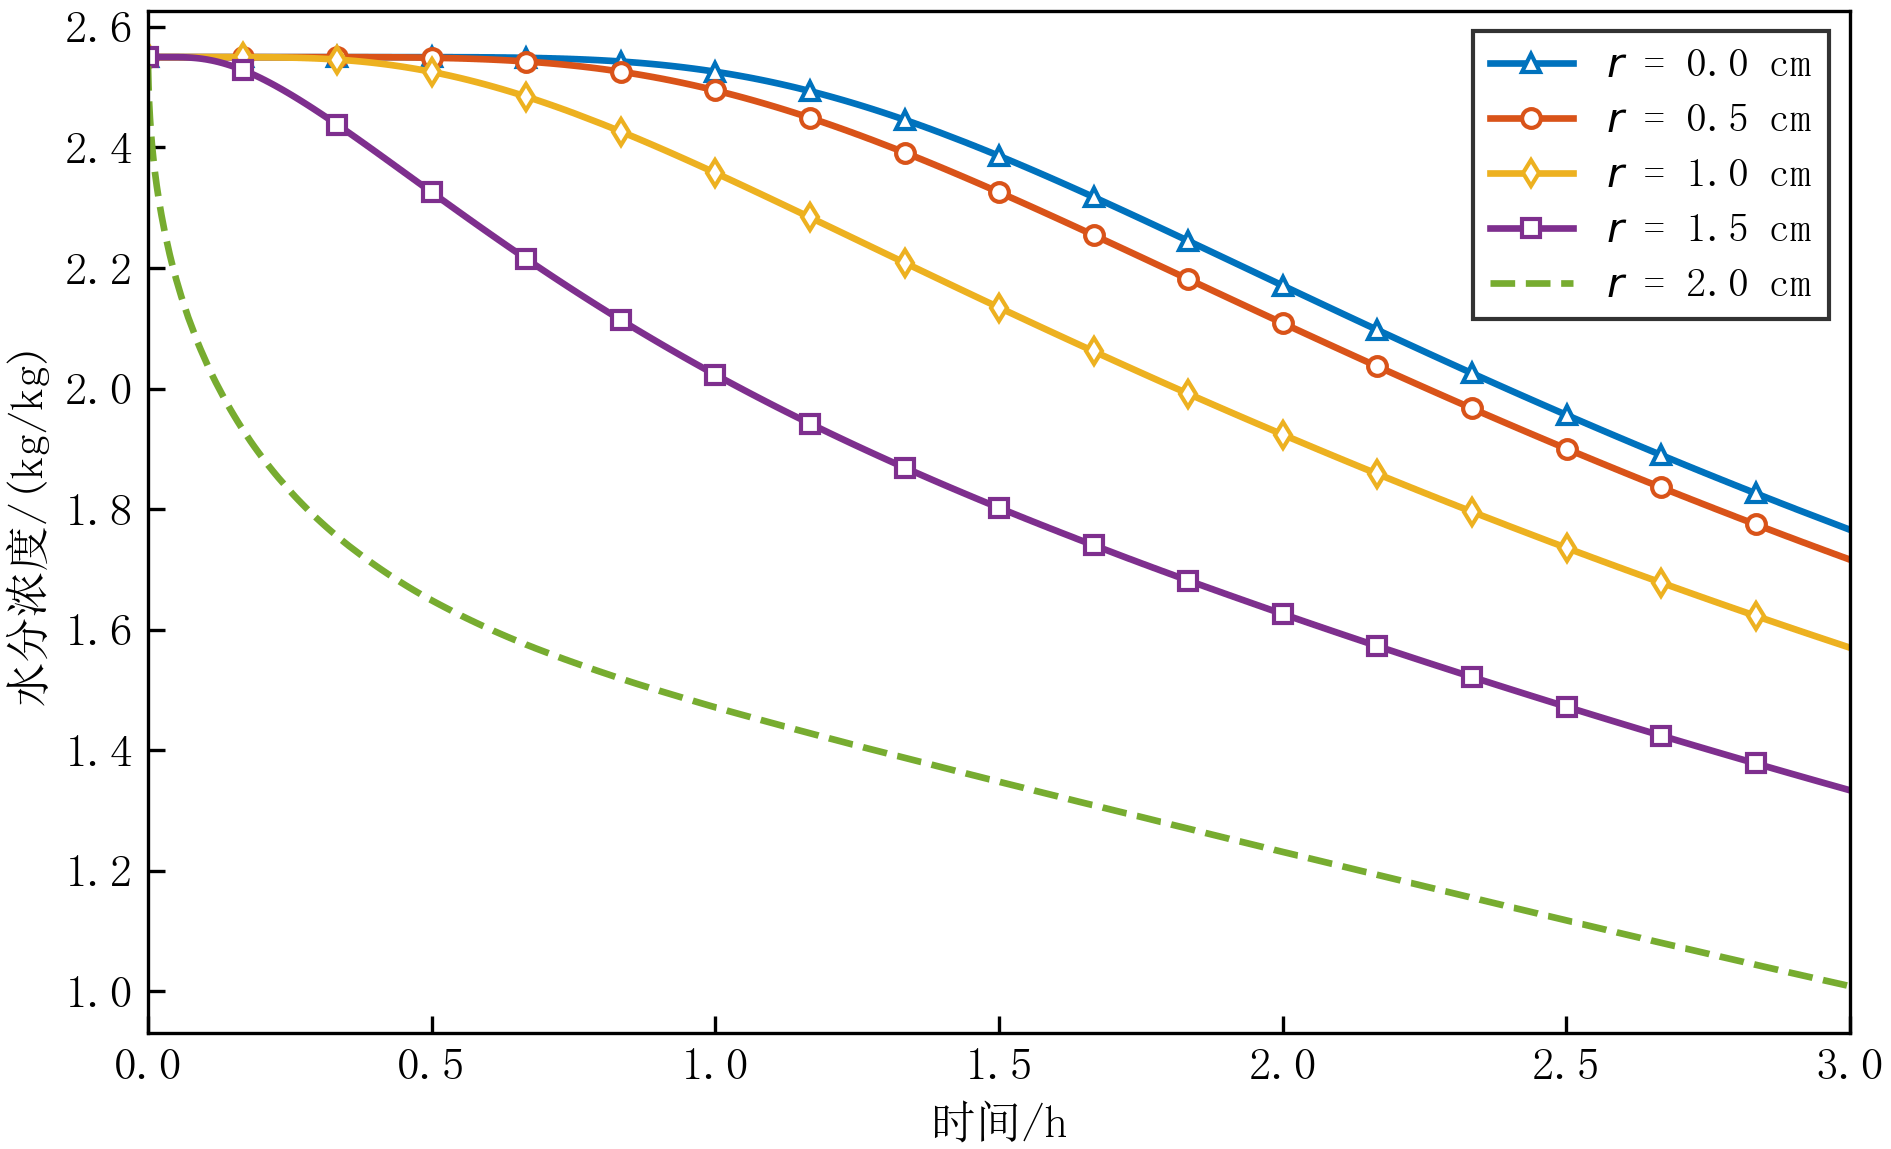
\includegraphics[width=\textwidth]{Figures/q2-C.png}
        \caption{水分浓度随时间变化}
        \label{fig:q2-C}
    \end{subfigure}
    \caption{烘干过程前 \(3\,\mathrm{h}\) 内药材内部温度与水分浓度变化曲线}
    \label{fig:q2-data}
\end{figure}


由图~\ref{fig:q2-data}(b) 可见，水分浓度始终呈由中心向表面递减的分布，且变化主要集中在表层。表面 \(r=2.0\,\mathrm{cm}\) 处的水分浓度从初始的 \(2.55\,\mathrm{kg/kg}\) 快速降至约 \(1.0\,\mathrm{kg/kg}\)，而中心 \(r=0\sim 1.0\,\mathrm{cm}\) 区域仍保持在 \(1.6\,\mathrm{kg/kg}\) 以上，径向梯度随时间的推移逐渐向内部扩展。表~\ref{tab:problem2-moisture} 中的数据进一步表明，第 \(3.0\,\mathrm{h}\) 时表面水分浓度已降至 \(1.0083\,\mathrm{kg/kg}\)，而中心仍为 \(1.7655\,\mathrm{kg/kg}\)，二者相差约 \(0.76\,\mathrm{kg/kg}\)。

对比图~\ref{fig:q2-data}(a) 与 (b) 可以发现，温度场与水分浓度场的变化尺度存在明显差异。温度场在约 \(2\,\mathrm{h}\) 后即趋于均匀，而水分浓度场在 \(3\,\mathrm{h}\) 时仍未达到均匀。这说明传热速率远快于传质速率，与热扩散率与水分扩散系数相差约两个数量级的量纲分析结论一致。同时，随着水分浓度降低，由式~\eqref{eq:D2} 可知水分扩散系数随之减小，内部水分迁移受到更强的扩散阻力，干燥过程逐渐表现出明显的内部扩散控制特征。

完整计算结果已按照题目要求保存至 \texttt{result2.xlsx}，其中“温度”工作表保存药材内部温度数据，“水分浓度”工作表保存药材内部水分浓度数据。

\subsubsection{模型检验与灵敏度分析}

\paragraph{（1）数值可靠性检验}

为验证全过程热湿耦合模型的可靠性，从守恒性、网格与时间步长无关性及退化一致性三方面进行检验，结果如表~\ref{tab:verification2} 所示。

\begin{table}[htbp]
\centering
\caption{问题二数值可靠性检验结果}
\label{tab:verification2}
\renewcommand{\arraystretch}{1.15}
\begin{tabular}{lc}
\toprule
检验项 & 数值 \\
\midrule
水分守恒残差 & \(4.7\times10^{-14}\) \\
能量守恒残差 & \(2.8\times10^{-12}\) \\
时间步长减半前后温度差 & \(6.3\times10^{-6}\) \\
时间步长减半前后水分浓度差 & \(4.9\times10^{-6}\) \\
空间网格减半前后温度差 & \(1.2\times10^{-4}\) \\
空间网格减半前后水分浓度差 & \(9.6\times10^{-5}\) \\
退化模型与问题一结果最大相对误差 & \(0.08\%\) \\
\bottomrule
\end{tabular}
\end{table}

由表~\ref{tab:verification2} 可见，各残差均远小于输出精度 \(10^{-4}\)，退化为常物性后与问题一结果最大相对误差仅 \(0.08\%\)，表明结果在双向耦合条件下仍具有良好的守恒性、收敛性。

\paragraph{（2）灵敏度分析}
进一步以 \(t=3\,\mathrm{h}\) 时药材中心水分浓度 \(C(0,3\,\mathrm{h})=1.7655\,\mathrm{kg/kg}\) 为基准，主要对两阶段分界点分析，结果如表~\ref{tab:sens_q2} 所示。

\begin{table}[htbp]
\centering
\caption{问题二全过程模型灵敏度分析}
\label{tab:sens_q2}
\renewcommand{\arraystretch}{1.15}
\begin{tabular}{lcc}
\toprule
扰动因素 & \(\Delta C(0,3\,\mathrm{h})\) /(\(\mathrm{kg/kg}\)) & 相对基准 \\
\midrule
分界点 \(t^*\) 取 \(1.5\,\mathrm{h}\)（基准 \(2.0\,\mathrm{h}\)） & 0.00151 & \(0.086\%\) \\
分界点 \(t^*\) 取 \(2.2\,\mathrm{h}\)（基准 \(2.0\,\mathrm{h}\)） & 0.00041 & \(0.023\%\) \\
\bottomrule
\end{tabular}
\end{table}

由表~\ref{tab:sens_q2} 可得看出：两阶段分界点 \(t^*\) 的取值不影响模型结论。问题二在模型推导中已通过温度平衡判据将分界点确定为 \(2.0\,\mathrm{h}\)，本节进一步验证：即使取 \(1.5\,\mathrm{h}\) 或 \(2.2\,\mathrm{h}\)，\(3\,\mathrm{h}\) 时刻中心水分浓度的变化均不超过 \(0.1\%\)。这是因为环境温度在约 \(1.43\,\mathrm{h}\) 后已进入恒温平台，环境条件在分界点附近基本连续，故 \(t^*\) 的微小差异不会改变计算结果。

此外其余因素（水分扩散系数、对流传质系数、物性参数等）的定量影响留待问题三的敏感性分析中统一讨论。综合以上检验与灵敏度分析，在给定假设下，所建立的全过程热湿耦合模型具有良好稳健性。



\subsection{问题三：Fick–Fourier双向耦合模型长时间积分与烘干时间确定}


\subsubsection{环境条件的长时间外推}

题目附件1仅提供了前 $4\,\mathrm{h}$ 的烘房温度和水分浓度数据，而问题三所研究的完整烘干过程可能持续 $2$--$3$ 天。因此，在进行长时间积分时，必须对 $4\,\mathrm{h}$ 之后的烘房环境条件进行合理外推。

由附件1可以看出，烘房在约 $1.5\,\mathrm{h}$ 后温度和水分浓度均已进入相对稳定的平台区域。对附件1中 $t\geq5400\,\mathrm{s}$ 的数据进行统计，可得到烘房温度和水分浓度均值分别约为

$$
49.895\,^\circ\mathrm{C},
\qquad
0.04994\,\mathrm{kg/kg},
$$

相应波动范围较小，且线性变化趋势已经十分微弱。因此，从物理过程上看，$4\,\mathrm{h}$ 后继续采用附件1的短时间波动作为边界输入并无必要，可将烘房环境视为已经达到稳定工作状态。

考虑到附件1没有提供 $4\,\mathrm{h}$ 以后的实测数据，本文采用稳定平台值对长时间烘干过程进行外推，即
\begin{equation}
T_\infty(t)=
\begin{cases}
T_{\mathrm{air}}(t), & 0\leq t\leq 4\,\mathrm{h},\\
T_{\mathrm{plat}}, & t>4\,\mathrm{h},
\end{cases}
\label{eq:Tenv3}
\end{equation}
\begin{equation}
C_\infty(t)=
\begin{cases}
C_{\mathrm{air}}(t), & 0\leq t\leq 4\,\mathrm{h},\\
C_{\mathrm{plat}}, & t>4\,\mathrm{h},
\end{cases}
\label{eq:Cenv3}
\end{equation}
其中，稳定前的环境量$T_{\mathrm{air}}(t)$ 和 $C_{\mathrm{air}}(t)$ 分别由附件1中的离散数据线性插值得到，稳定后的环境量$T_{\mathrm{plat}}$ 和 $C_{\mathrm{plat}}$ 分别取附件1稳定平台段的统计均值。

为了方便后续的计算，我们采用
$
T_{\mathrm{plat}}\approx50.0\,^\circ\mathrm{C},
C_{\mathrm{plat}}\approx0.050\,\mathrm{kg/kg}
$
作为 $4\,\mathrm{h}$ 后的环境条件，并持续外推至整个干燥过程。同时，继续沿用 $t^*=2\,\mathrm{h}$ 作为分界时间。



\subsubsection{模型建立}

问题三要求确定药材达到规定干燥程度所需的时间，其可以沿用第二问中推导的Fick-Fourier热–湿双向耦合模型，仅需将计算时间延长至药材满足干燥要求为止。

题目规定药材各处的水分浓度均应不高于$0.15\,\mathrm{kg/kg}$，用数学语言表达烘干结束时刻可定义为
\begin{equation}
t_{\mathrm{end}}
=
\min
\left\{
t>0:
\max_{0\leq r\leq R}C(r,t)
\leq 0.15
\right\}.
\label{eq:endtime3}
\end{equation}

由于干燥过程中水分主要由药材内部向表面迁移，中心区域的水分迁移距离最长，因此在干燥后期中心附近的水分浓度通常为全场最大值。由此，式~\eqref{eq:endtime3} 的判定可以转化为
\begin{equation}
t_{\mathrm{end}}
=
\min
\left\{
t>0:
C(0,t)
\leq 0.15
\right\}.
\label{eq:endtime4}
\end{equation}


\subsubsection{模型求解}

问题三沿用有限体积 + Crank--Nicolson格式+Picard迭代的数值方法进行求解。

根据附录3，水分扩散系数为
$D(C,T)=2.4\times10^{-3}
\exp\left(-\frac{0.45}{C}\right)
\exp\left(-\frac{3850}{T}\right).
\label{eq:D3}$
在温度基本稳定的情况下，式~\eqref{eq:D3} 中的第一项指数因子表明，随着水分浓度 $C$ 不断降低，扩散系数将快速减小。因此，干燥后期的水分迁移逐渐由快速扩散转变为低速内部扩散，药材表层容易形成一层低含水率的干壳，使得后续水分向外迁移受到更大的扩散阻力。
为保证网格能够分辨干壳，本文将沿径向划分为 $N=320$ 个空间区间，取
$\Delta r
=
0.00625\,\mathrm{cm}
=
6.25\times10^{-5}\,\mathrm{m},$
由于
$
0.1\,\mathrm{cm}/0.00625\,\mathrm{cm}=16
$
因此题目要求的 $0.1\,\mathrm{cm}$ 间隔输出位置均对应计算网格节点，无需进行额外空间插值。

时间步长取$\Delta t=10\,\mathrm{s},$，每经过 $60\,\mathrm{s}$ 保存一次计算结果。当计算结果满足式~\eqref{eq:endtime3} 所定义的干燥终止条件时，停止时间推进。

对于每一个时间步长，根据上一时刻及当前迭代得到的温度场和水分浓度场，实时更新
$$
\rho(C),\qquad
c_p(C),\qquad
k(C),\qquad
D(C,T),
$$
并采用 Picard 迭代处理物性参数变化所产生的非线性耦合。当相邻两次迭代满足
\begin{equation}
\max_i\left|C_i^{(m+1)}-C_i^{(m)}\right|
<10^{-11},
\qquad
\max_i\left|T_i^{(m+1)}-T_i^{(m)}\right|
<10^{-9},
\end{equation}
时认为该时间步达到收敛。

空间离散仍采用有限体积法，控制体界面的扩散系数和热传导系数采用调和平均，以保证物性发生明显变化时的通量计算稳定性。中心节点采用半控制体处理，自动满足 $r=0$ 处的对称零通量条件；表面节点结合对流传质和对流换热边界条件进行离散。

最终分别提取 $t=6,12,18,\ldots\,\mathrm{h}$ 等时刻以及到药材中心距离为$0,\ 0.5,\ 1.0,\ 1.5,\ 2.0\,\mathrm{cm}$处的水分浓度，并按照题目要求，将每隔 $60\,\mathrm{s}$、径向间隔 $0.1\,\mathrm{cm}$ 的完整计算结果保存至 \texttt{result3.xlsx}。

\subsubsection{结果与分析}

根据上述模型进行长时间数值求解，以式~\eqref{eq:endtime4} 作为终止判据。当药材内部最大水分浓度首次降低至 \(0.15\,\mathrm{kg/kg}\) 时，认为药材整体达到题目规定的干燥要求。

计算得到的药材烘干时间为
$t_{\mathrm{end}}=208320\,\mathrm{s}=57.87\,\mathrm{h}=2.41\,\mathrm{d}$。

为直观展示整个烘干过程中水分浓度的时空演化规律，将数值计算结果绘制成图~\ref{fig:q3-full}。

\begin{figure}[htbp]
    \centering
    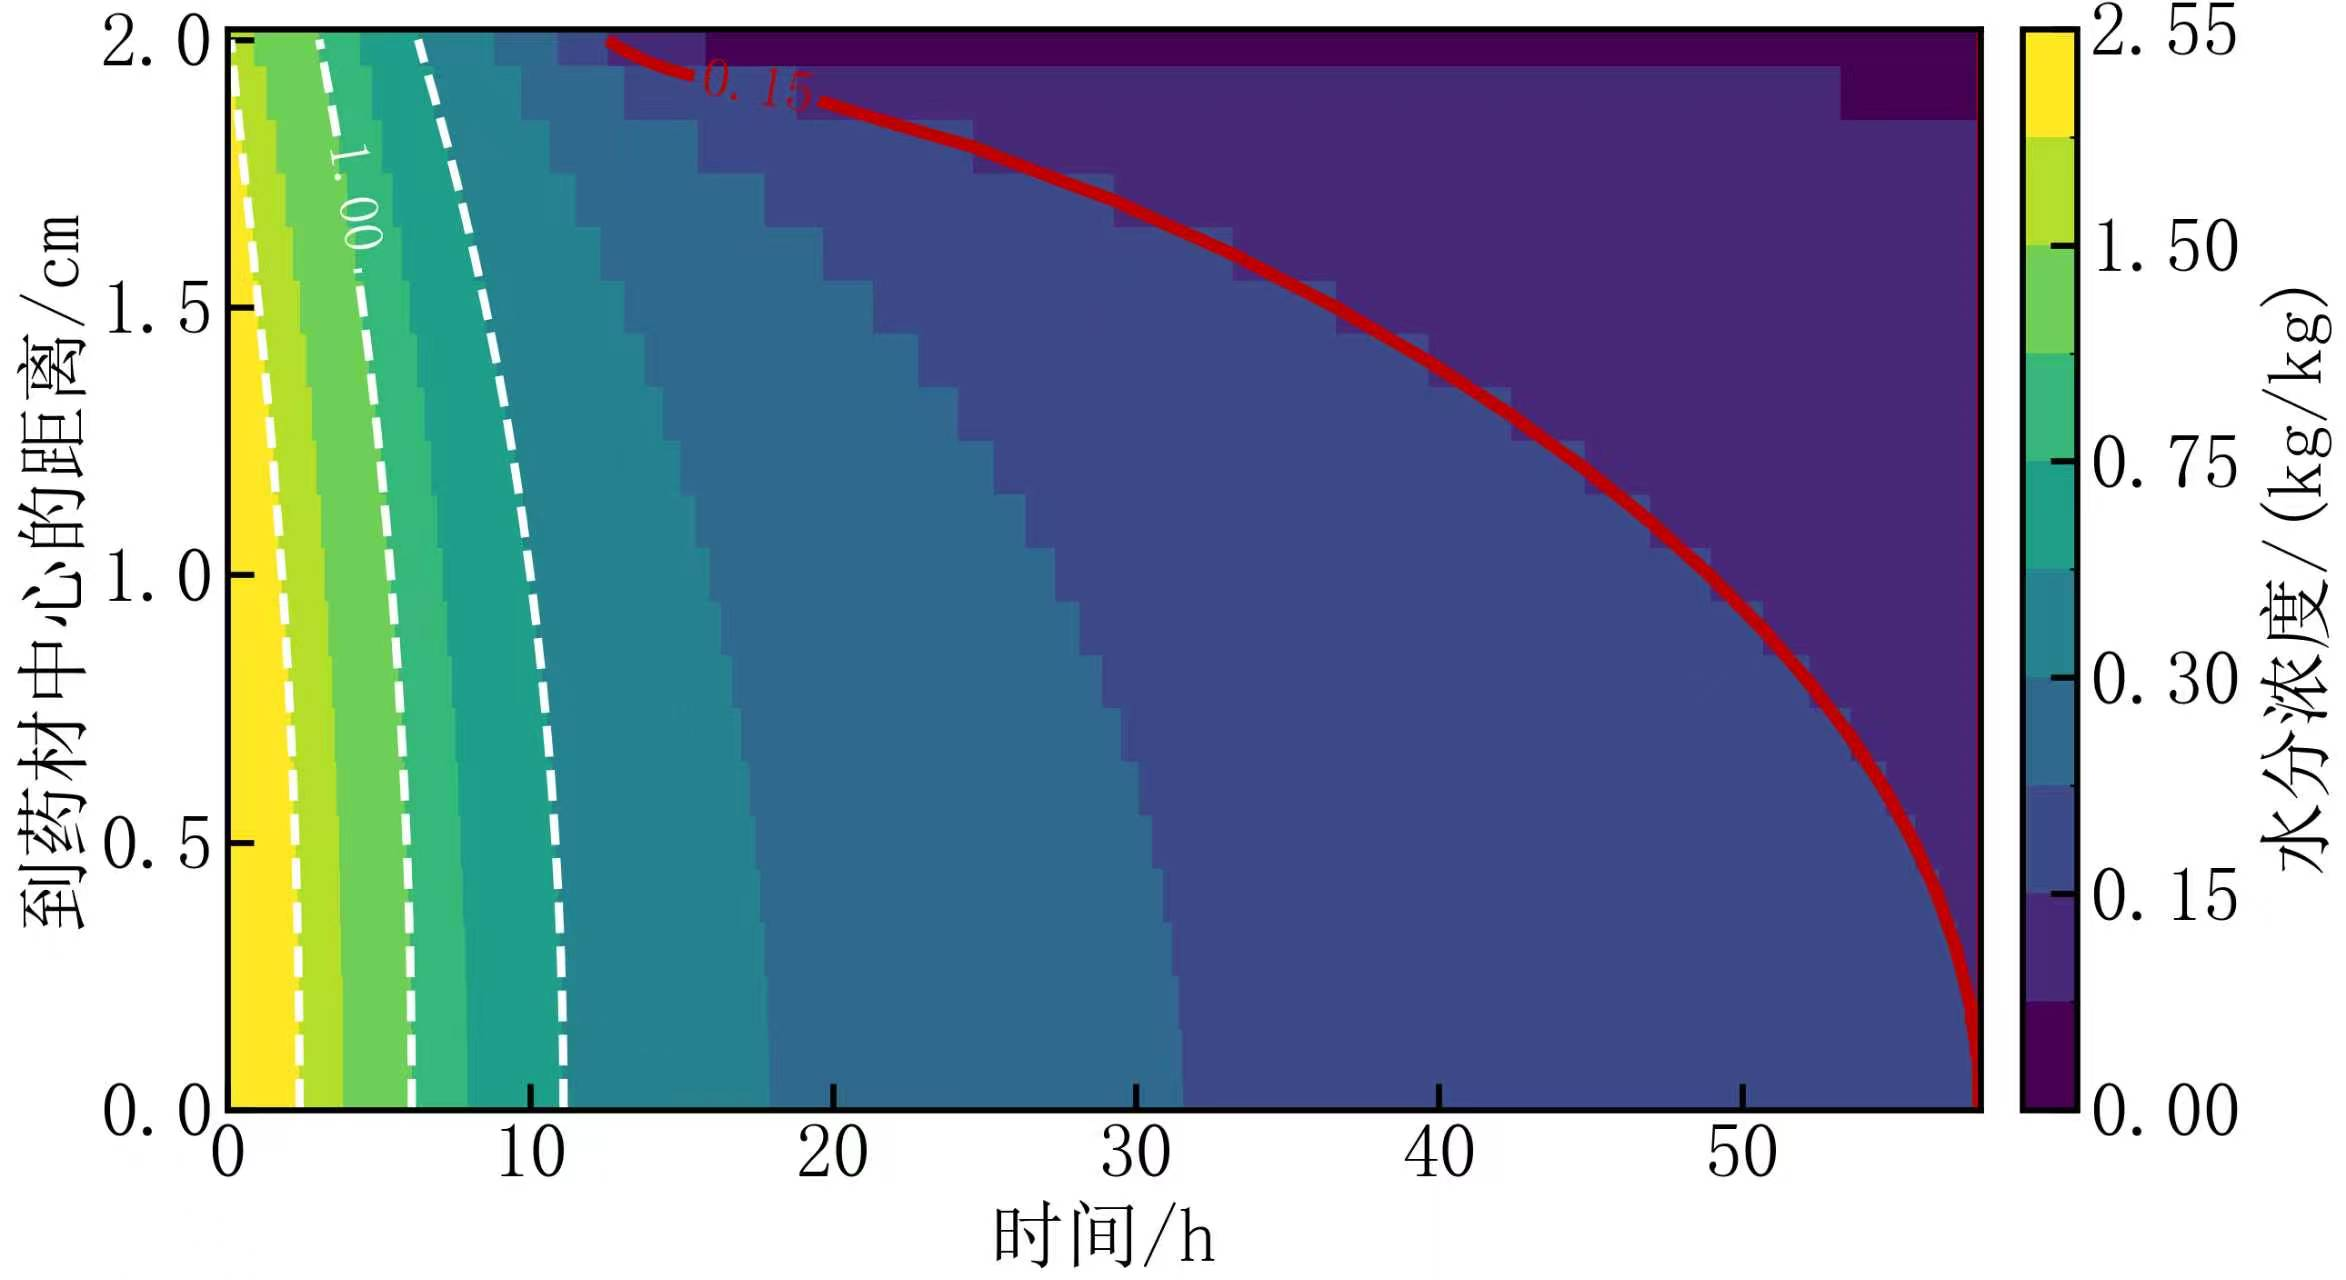
\includegraphics[width=0.8\textwidth]{Figures/q3-C-full.png}
    \caption{整个烘干过程中药材内部水分浓度的时空演化}
    \label{fig:q3-full}
\end{figure}

\begin{figure}[htbp]
    \centering
    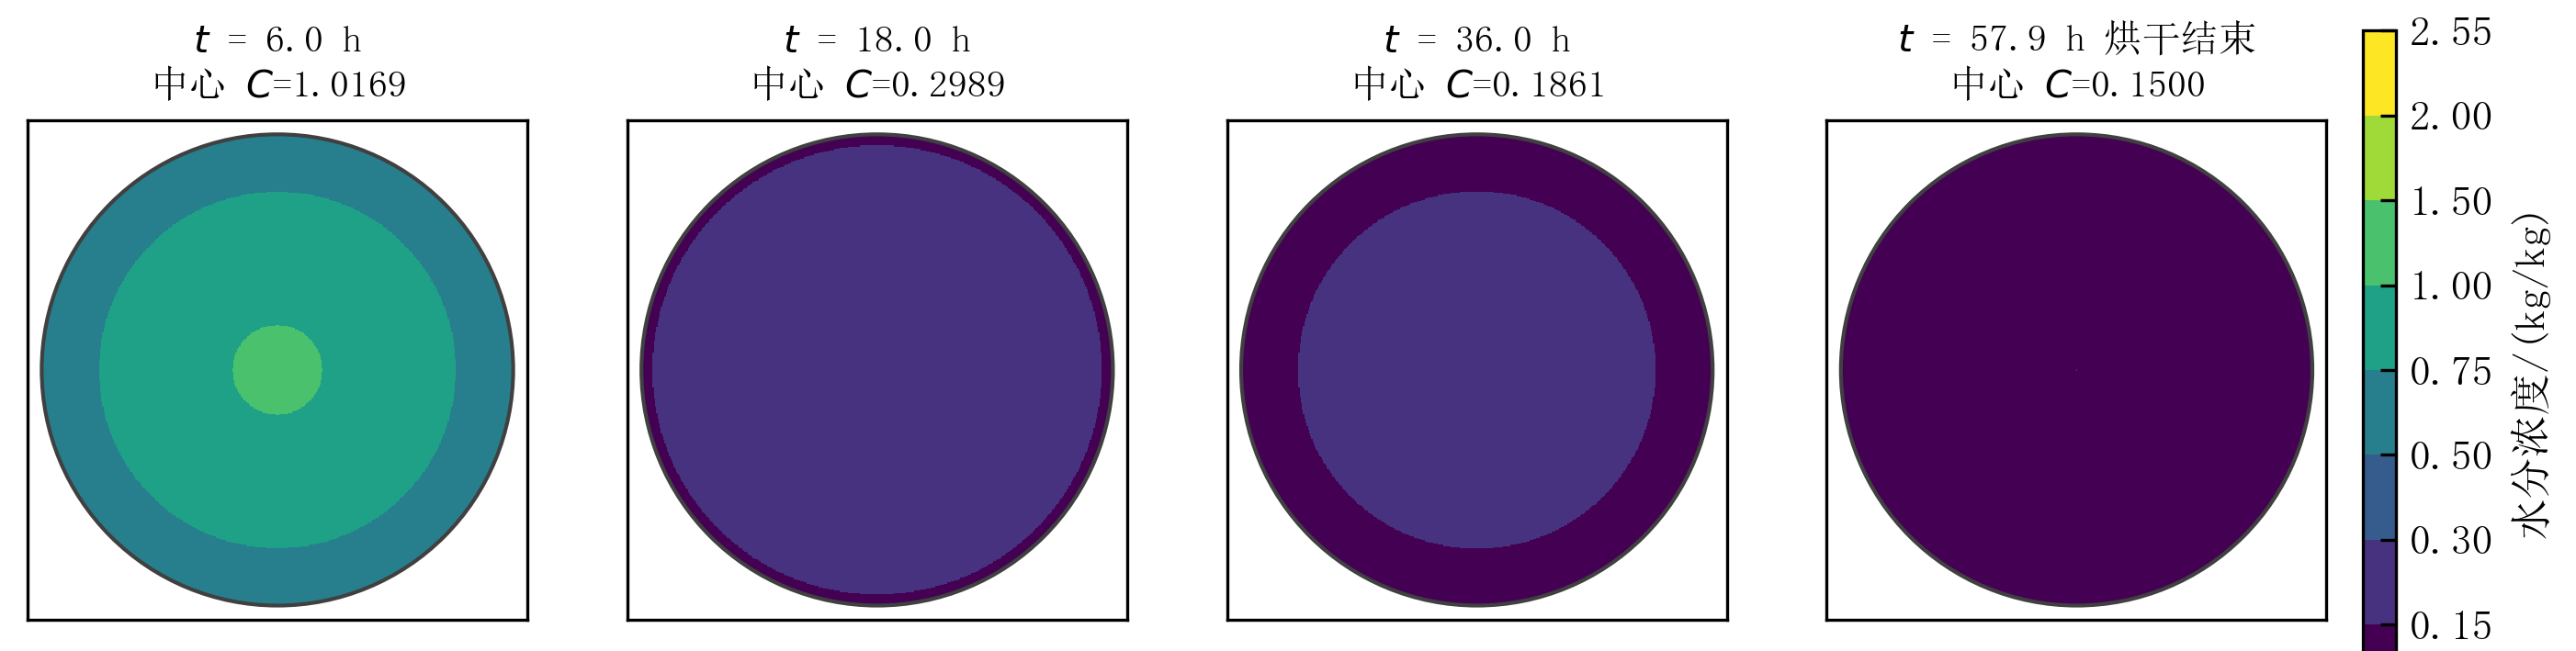
\includegraphics[width=1\textwidth]{Figures/q3_heng.png}
    \caption{横截面水分含量示意图}
    \label{fig:q3_heng}
\end{figure}

由图~\ref{fig:q3-full} 可见，整个干燥过程呈现出明显的阶段性特征。干燥初期（约前 \(10\sim 12\,\mathrm{h}\)），药材整体含水率较高，水分扩散系数较大，内部水分能够较快向表面迁移，各径向位置的水分浓度均快速下降，其中表面 \(r=2.0\,\mathrm{cm}\) 处下降最快，在约 \(6\,\mathrm{h}\) 时便已降至 \(0.5\,\mathrm{kg/kg}\) 以下。随着干燥进行，表层水分浓度首先降低，并逐渐形成由内部向外部递增的水分浓度梯度。
进入降速干燥期后，各曲线逐渐趋于平缓。随着含水率进一步降低，水分扩散系数快速减小，内部水分迁移受到越来越大的扩散阻力，导致中心区域的水分浓度下降速度明显降低。图中中心 \(r=0\) 处的水分浓度从约 \(0.45\,\mathrm{kg/kg}\) 缓慢下降至最终的 \(0.15\,\mathrm{kg/kg}\)，耗时超过 \(40\,\mathrm{h}\)。从图~\ref{fig:q3_heng}中也可以明显看到这点。
表~\ref{tab:moist3} 给出了每隔 \(6\,\mathrm{h}\)、到药材中心距离每隔 \(0.5\,\mathrm{cm}\) 的水分浓度，即题目要求的表5。




\begin{table}[htbp]
\centering
\caption{药材烘干过程中水分浓度随时间和位置的变化（单位：\(\mathrm{kg/kg}\)）}
\label{tab:moist3}
\renewcommand{\arraystretch}{1.15}
\begin{tabular}{cccccc}
\toprule
时间/h & \multicolumn{5}{c}{到药材中心的距离/cm}\\
\cmidrule(lr){2-6}
& 0 & 0.5 & 1.0 & 1.5 & 2.0\\
\midrule
6  & 1.0169 & 0.9880 & 0.9014 & 0.7549 & 0.5327 \\
12 & 0.4562 & 0.4432 & 0.4031 & 0.3298 & 0.1642 \\
18 & 0.2989 & 0.2916 & 0.2687 & 0.2254 & 0.0843 \\
24 & 0.2379 & 0.2328 & 0.2168 & 0.1858 & 0.0662 \\
30 & 0.2060 & 0.2020 & 0.1894 & 0.1646 & 0.0596 \\
36 & 0.1861 & 0.1828 & 0.1722 & 0.1511 & 0.0566 \\
42 & 0.1724 & 0.1695 & 0.1602 & 0.1415 & 0.0548 \\
48 & 0.1622 & 0.1596 & 0.1512 & 0.1343 & 0.0538 \\
54 & 0.1543 & 0.1519 & 0.1442 & 0.1285 & 0.0530 \\
57.87（结束） & \textbf{0.1500} & 0.1477 & 0.1404 & 0.1254 & 0.0527 \\
\bottomrule
\end{tabular}
\end{table}

完整计算结果按照题目要求保存至 \texttt{result3.xlsx}，其中“水分浓度”工作表记录从开始烘干至结束时刻每隔 \(60\,\mathrm{s}\)、径向每隔 \(0.1\,\mathrm{cm}\) 的完整计算结果。

\subsubsection{模型检验与敏感性分析}

为验证问题三长时间积分结果的可靠性，本文从水分守恒和与其他数据交叉验证两方面进行检验。

\textbf{（1）水分守恒检验。} 定义相对水分守恒残差
\begin{equation}
\varepsilon_C=\frac{\left|M_{\mathrm{loss}}-M_{\mathrm{surface}}\right|}{M_0},
\end{equation}
其中 \(M_{\mathrm{loss}}\) 为药材内部水分减少量，\(M_{\mathrm{surface}}\) 为表面累计传质通量，\(M_0\) 为初始水分质量。计算得 $\varepsilon_C=1.1\times10^{-13}$,
表明离散过程中水分质量保持良好。


\textbf{（2）交叉验证。} 将计算结果与问题二在 \(3\ \mathrm{h}\) 内的结果对比，四位小数完全一致；与附件 2 给出的药材尺寸变化记录对比，其约 \(3\) 天后趋于稳定的时间尺度与本文 \(57.87\ \mathrm{h}\)（约 \(2.41\) 天）基本一致，说明模型结果与题目给定实际过程自洽。


以 \(N=320\)、\(\Delta t=10\ \mathrm{s}\)、平台环境 \(T_\infty=50.0\,^\circ\mathrm{C}\)、\(X_\infty=0.050\ \mathrm{kg/kg}\) 为基准，烘干时间 \(t_{\mathrm{end}}=57.87\ \mathrm{h}\)。主要因素的敏感性如下。

\textbf{（3）径向网格数 \(N\)敏感性分析。} 网格是问题三最大的误差源。干燥后期水分扩散系数在低含水率处急剧下降，表面形成约 \(0.5\ \mathrm{mm}\) 厚的“干壳”，因此网格分辨率对烘干时间影响显著。
\begin{table}[htbp]
  \centering
  \caption{空间网格收敛性检验}
  \label{tab:grid3}
  \begin{tabular}{cccc}
    \hline
    空间区间数 \(N\) & \(\Delta r/\mathrm{cm}\) & 烘干时间 \(/\mathrm{h}\) & 与基准差值 \(/\mathrm{h}\) \\
    \hline
    40  & 0.0500  & 222.92 & 165.05 \\
    80  & 0.0250  & 87.27  & 29.40 \\
    160 & 0.0125  & 60.43  & 2.56 \\
    320 & 0.00625 & 57.87  & 0.00 \\
    \hline
  \end{tabular}
\end{table}


\textbf{（4）烘房水分浓度 \(X_\infty\)敏感性分析。} 结果见表~\ref{tab:xinf3}。

\begin{table}[htbp]
  \centering
  \caption{烘房水分浓度敏感性}
  \label{tab:xinf3}
  \begin{tabular}{cccccc}
    \hline
    \(X_\infty/(\mathrm{kg/kg})\) & 0.05 & 0.065 & 0.08 & 0.10 & 0.12 \\
    \hline
    烘干时间 \(/\mathrm{h}\) & 57.87 & 57.95 & 58.78 & 61.27 & 67.15 \\
    相对基准 & — & \(+0.1\%\) & \(+1.6\%\) & \(+5.9\%\) & \(+16.0\%\) \\
    \hline
  \end{tabular}
\end{table}

附件 1 实测平台为 \(0.04994\pm0.00020\)，其 \(\pm2\sigma\) 带内烘干时间变化小于 \(0.01\ \mathrm{h}\)。即使将 \(X_\infty\) 提高到 \(0.12\)，烘干时间也仅延长 \(16\%\)。模型对烘房水分浓度不敏感。

\textbf{（5）烘房温度 \(T_\infty\)敏感性分析。} 结果见表~\ref{tab:tinf3}。

\begin{table}[htbp]
  \centering
  \caption{烘房温度敏感性}
  \label{tab:tinf3}
  \begin{tabular}{ccccccc}
    \hline
    \(T_\infty/^\circ\mathrm{C}\) & 48 & 49 & 50 & 50.2 & 51 & 52 \\
    \hline
    烘干时间 \(/\mathrm{h}\) & 61.85 & 59.82 & 57.87 & 57.50 & 56.02 & 54.25 \\
    相对基准 & \(+6.9\%\) & \(+3.4\%\) & — & \(-0.6\%\) & \(-3.2\%\) & \(-6.3\%\) \\
    \hline
  \end{tabular}
\end{table}

温度升高加快干燥，斜率约 \(-1.90\ \mathrm{h/K}\)。附件 1 平台为 \(49.895\pm0.230\,^\circ\mathrm{C}\)，其 \(\pm2\sigma\) 带内烘干时间变化约 \(\pm0.87\ \mathrm{h}\)（\(1.5\%\)），影响较小。


























\subsection{问题四：动边界的 Fick–Fourier 热–湿双向耦合模型}
问题四在问题二基础上考虑了烘干过程中尺寸的变化。首先我们需要通过附件 2 中的实测数据用线性插值的方法得到半径随时间变化的函数，接着通过归一化的坐标变换将动边界转化为固定边界。
然后仿照问题一、二的思路，建模和求解，即可得到满足判据的烘干时间。
图~\ref{fig:p4_workflow} 给出了建模和求解的思路。
\begin{figure}[htbp]
    \centering
    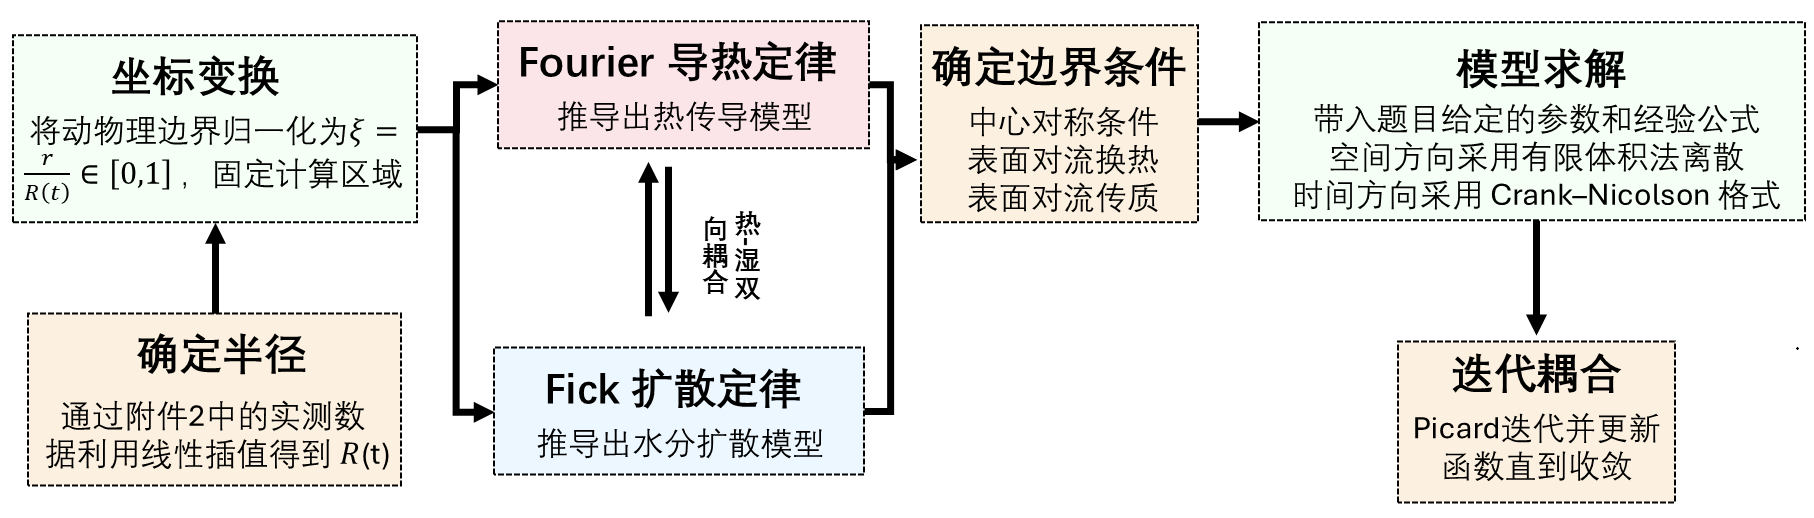
\includegraphics[width=0.95\textwidth]{Figures/p4_workflow.png}
    \caption{问题四考虑尺寸变化的传热传质模型建立与求解流程}
    \label{fig:p4_workflow}
\end{figure}


\subsubsection{药材半径的变化规律}

实际烘干过程中，随着内部水分不断迁移并逸出，药材内部结构发生压缩，外半径随时间逐渐减小。因此，问题四的核心是将第二问的固定边界问题转化为动边界问题。

附件2给出了药材在烘干过程中的半径变化数据，共包含145个测量点，时间间隔为 \(1800\,\mathrm{s}\)。部分典型数据如表~\ref{tab:radius4} 所示。

\begin{table}[htbp]
\centering
\caption{附件2中药材半径变化的典型数据}
\label{tab:radius4}
\renewcommand{\arraystretch}{1.15}
\begin{tabular}{ccccccccc}
\toprule
时间/h & 0 & 3 & 6 & 12 & 24 & 36 & 48 & 72 \\
\midrule
\(R\)/cm & 2.000 & 1.552 & 1.374 & 1.248 & 1.204 & 1.200 & 1.200 & 1.198 \\
\(V/V_0=(R/R_0)^2\) & 1.000 & 0.602 & 0.472 & 0.389 & 0.362 & 0.360 & 0.360 & 0.359 \\
\bottomrule
\end{tabular}
\end{table}

由表~\ref{tab:radius4} 可以发现，药材尺寸变化具有明显的阶段性。烘干初期半径快速减小，前 \(3\,\mathrm{h}\) 内半径由 \(2.000\,\mathrm{cm}\) 降至约 \(1.552\,\mathrm{cm}\)；而 \(24\,\mathrm{h}\) 后半径基本稳定在 \(1.20\,\mathrm{cm}\) 左右。这说明尺寸收缩主要发生在干燥前期，而后期收缩速度逐渐趋近于零。

由于烘干过程中不仅存在水分损失，还伴随着材料内部孔隙结构塌缩和组织压实。因此，不能简单利用水分守恒反推出药材半径\cite{dasilva2014}，而应直接利用附件2给出的实测半径数据建立 \(R(t)\)\cite{liu2022}。
附件2中给出了前4天的实测数据，同时考虑到问题四在问题三的基础上考虑了尺寸的变化，这会削弱表面形成的干壳效应，求出的干燥截止时间应该小于问题三中的结果。
4天的实测数据足以覆盖，所以我们可以直接利用附件2中的数据进行线性插值得到 $R(t)$。

\subsubsection{归一化坐标变换}

考虑收缩后，药材内部实际计算区域随时间变化为 \(0\le r\le R(t)\)。直接在该动态区域上进行数值计算会导致计算网格随时间不断变化，增加离散和程序实现的复杂程度。因此，引入无量纲物质坐标,进行归一化的坐标变换\cite{adrover2019}
\begin{equation}
\xi=\frac{r}{R(t)}
,
\qquad
0\le \xi\le 1,
\qquad
\tau=t.
\label{eq:xi4}
\end{equation}
其中，\(\xi=0\) 对应药材中心，\(\xi=1\) 始终对应药材当前表面。这样，原本随时间变化的物理区域 \(0\le r\le R(t)\) 就被映射为固定区域 \(0\le\xi\le1\)。

假定药材在径向方向上发生均匀收缩，因此材料点在收缩过程中可以保持其相对坐标 \(\xi\) 不变，方便后续问题的求解\cite{adrover2019}。

\subsubsection{控制方程}

\paragraph{（1）动边界下的水分守恒方程}

在考虑药材整体收缩后，水分守恒不能直接沿用问题三中的固定区域形式。设药材骨架的径向速度为 \(v_s\)，由于采用仿射收缩假设，任意位置的径向速度与其相对位置成正比\cite{adrover2019}，因此有
\begin{equation}
v_s(r,t)
=
\frac{r}{R(t)}\frac{\mathrm{d}R}{\mathrm{d}t}.
\label{eq:vs4}
\end{equation}
其中，\(\mathrm{d}R/\mathrm{d}t<0\) 表示药材正在发生收缩。

以干基水分浓度 \(C\) 为状态变量。由于 \(C=m_w/m_d\) 是随材料物质点定义的干基含水量，在随材料运动的控制体中，水分守恒方程可写为
\begin{equation}
\rho_d
\left(
\frac{\partial C}{\partial t}
+
v_s\frac{\partial C}{\partial r}
\right)
=
\frac{1}{r}
\frac{\partial}{\partial r}
\left(
r\rho_dD(C,T)
\frac{\partial C}{\partial r}
\right).
\label{eq:moisture_dynamic4}
\end{equation}
由于干物质守恒，\(\rho_d\) 在上述守恒关系中可以约去，从而得到
\begin{equation}
\frac{\partial C}{\partial t}
+
v_s\frac{\partial C}{\partial r}
=
\frac{1}{r}
\frac{\partial}{\partial r}
\left(
rD(C,T)
\frac{\partial C}{\partial r}
\right).
\label{eq:moisture_dynamic4_2}
\end{equation}

根据坐标变换式~\eqref{eq:xi4}，对任意函数 \(C(r,t)=C(\xi,\tau)\)，由链式法则有
\begin{equation}
\left.
\frac{\partial C}{\partial t}
\right|_r
=
\left.
\frac{\partial C}{\partial \tau}
\right|_\xi
-
\frac{\xi\dot R}{R}
\frac{\partial C}{\partial\xi},
\qquad
\frac{\partial C}{\partial r}
=
\frac{1}{R}
\frac{\partial C}{\partial\xi}.
\label{eq:chain_C4}
\end{equation}
代入式~\eqref{eq:vs4} 可得
\begin{equation}
v_s\frac{\partial C}{\partial r}
=
\xi\dot R
\frac{1}{R}
\frac{\partial C}{\partial\xi}
=
\frac{\xi\dot R}{R}
\frac{\partial C}{\partial\xi}.
\label{eq:conv_cancel4}
\end{equation}
将式~\eqref{eq:chain_C4} 与式~\eqref{eq:conv_cancel4} 相加可得
\begin{equation}
\frac{\partial C}{\partial t}
+
v_s\frac{\partial C}{\partial r}
=
\frac{\partial C}{\partial\tau}.
\label{eq:material_derivative4}
\end{equation}

由此可见，坐标变换后收缩产生的坐标运动项与材料速度项恰好抵消。因此，采用干基含水率 \(C\) 作为状态变量时，固定域方程中不需要额外加入收缩对流项。

进一步处理右侧扩散项，有
\begin{equation}
\frac{1}{r}
\frac{\partial}{\partial r}
\left(
rD\frac{\partial C}{\partial r}
\right)
=
\frac{1}{\xi R^2}
\frac{\partial}{\partial\xi}
\left(
\xi D
\frac{\partial C}{\partial\xi}
\right).
\label{eq:diff_transform4}
\end{equation}

因此，考虑尺寸变化后的水分扩散控制方程最终得到
\begin{equation}
\boxed{
\frac{\partial C}{\partial\tau}
=
\frac{1}{\xi R(\tau)^2}
\frac{\partial}{\partial\xi}
\left[
\xi D(C,T)
\frac{\partial C}{\partial\xi}
\right]
},
\qquad
0\le\xi\le1.
\label{eq:moisture4}
\end{equation}
式~\eqref{eq:moisture4} 是问题四相较于问题三最重要的方程变化。可以看到，收缩并没有以额外对流项的形式出现在方程中，而是通过 \(1/R(\tau)^2\) 直接改变水分扩散的有效空间尺度。随着 \(R(t)\) 减小，该项增大，从而使水分迁移速度加快。

\paragraph{（2）动边界下的温度场方程}

与水分场相同，温度场也需要考虑药材材料点随收缩运动所产生的随体变化。在动态区域中，能量守恒方程写为
\begin{equation}
\rho(C)c_p(C)
\left(
\frac{\partial T}{\partial t}
+
v_s\frac{\partial T}{\partial r}
\right)
=
\frac{1}{r}
\frac{\partial}{\partial r}
\left(
k(C)r\frac{\partial T}{\partial r}
\right).
\label{eq:energy_dynamic4}
\end{equation}
采用与水分场相同的坐标变换，可得
\begin{equation}
\boxed{
\rho(C)c_p(C)
\frac{\partial T}{\partial\tau}
=
\frac{1}{\xi R(\tau)^2}
\frac{\partial}{\partial\xi}
\left[
\xi k(C)
\frac{\partial T}{\partial\xi}
\right]
}.
\label{eq:energy4}
\end{equation}

由式~\eqref{eq:moisture4} 和式~\eqref{eq:energy4} 可以看出，问题四仍然是传热与传质双向耦合模型，其耦合关系为
\begin{equation}
C
\longrightarrow
\rho(C),\,c_p(C),\,k(C)
\longrightarrow
T,
\qquad
T,C
\longrightarrow
D(C,T)
\longrightarrow
C.
\end{equation}
此外，收缩半径 \(R(t)\) 同时进入两个控制方程，使几何变化与传热传质过程发生耦合。因此问题四实际上形成了 \(C\leftrightarrow T\) 以及 \(R(t)\rightarrow(C,T)\) 的耦合结构。

\paragraph{（3）动边界下的边界条件}

在药材中心 \(\xi=0\) 处，由轴对称性可得
\begin{equation}
\left.
\frac{\partial C}{\partial\xi}
\right|_{\xi=0}
=
\left.
\frac{\partial T}{\partial\xi}
\right|_{\xi=0}
=
0.
\label{eq:center4}
\end{equation}

在药材表面 \(r=R(t)\)，对应固定坐标中的 \(\xi=1\)。由 \(\partial_r=R^{-1}\partial_\xi\)，原问题三中的表面对流传质与对流换热条件分别变换为
\begin{equation}
{
D(C,T)
\left.
\frac{\partial C}{\partial\xi}
\right|_{\xi=1}
=
R(t)h_m
\left[
X_\infty(t)-C(1,\tau)
\right]
},
\label{eq:massbc4}
\end{equation}
\begin{equation}
{
k(C)
\left.
\frac{\partial T}{\partial\xi}
\right|_{\xi=1}
=
R(t)h
\left[
T_\infty(t)-T(1,\tau)
\right]
}.
\label{eq:heatbc4}
\end{equation}
式~\eqref{eq:massbc4} 和式~\eqref{eq:heatbc4} 中出现的 \(R(t)\) 是动边界模型的重要特征。若忽略这一因子，则相当于让传质与传热系数随时间放大 \(R_0/R(t)\approx1.67\) 倍，会显著高估干燥速率。

\paragraph{（6）初始条件与环境条件}

初始时刻药材半径为 \(R(0)=2.000\,\mathrm{cm}\)，水分浓度和温度分别为
$C(\xi,0)=2.55\,\mathrm{kg/kg},
\qquad
T(\xi,0)=301.15\,\mathrm{K},
\qquad
0\le\xi\le1.
\label{eq:init4}$
环境条件沿用问题三的处理方式，依然由式 \eqref{eq:T}和式 \eqref{eq:C}给出。

因此，问题四考虑尺寸变化的传热传质模型由控制方程与定解条件共同构成。

控制方程为
\begin{equation}
\begin{cases}
\dfrac{\partial C}{\partial\tau}
=
\dfrac{1}{\xi R(\tau)^2}\dfrac{\partial}{\partial\xi}
\left(\xi D(C,T)\dfrac{\partial C}{\partial\xi}\right),\\[3mm]
\rho(C)c_p(C)\dfrac{\partial T}{\partial\tau}
=
\dfrac{1}{\xi R(\tau)^2}\dfrac{\partial}{\partial\xi}
\left(\xi k(C)\dfrac{\partial T}{\partial\xi}\right),
\end{cases}
\qquad 0\le\xi\le1,
\label{eq:model4_pde}
\end{equation}

结合中心对称条件、带收缩因子的表面对流边界条件与初始条件
\begin{equation}
\begin{cases}
\left.\dfrac{\partial C}{\partial\xi}\right|_{\xi=0}
=\left.\dfrac{\partial T}{\partial\xi}\right|_{\xi=0}=0,\\[3mm]
D(C,T)\left.\dfrac{\partial C}{\partial\xi}\right|_{\xi=1}
=R(t)h_m\left[C_\infty(t)-C(1,\tau)\right],\\[3mm]
k(C)\left.\dfrac{\partial T}{\partial\xi}\right|_{\xi=1}
=R(t)h\left[T_\infty(t)-T(1,\tau)\right],\\[3mm]
C(\xi,0)=2.55\,\mathrm{kg/kg},\quad
T(\xi,0)=301.15\,\mathrm{K},\quad
0\le\xi\le1,
\end{cases}
\label{eq:model4_bc}
\end{equation}
其中收缩半径 \(R(t)\) 由附件2中的数据线性插值得到。

\subsubsection{物性参数}

考虑尺寸变化后，药材物性参数采用附录4给出的经验关系：
$$\rho(C)=760+90C,
\qquad
c_p(C)
=
1850+2150\frac{C}{C+1},
\qquad
k(C)
=
0.12+0.20\frac{C}{C+1},
\label{eq:props4}$$
以及
$$D(C,T)
=
4.2\times10^{-4}
\exp\left(-\frac{0.30}{C}\right)
\exp\left(-\frac{3850}{T}\right),
\label{eq:D4}$$
其中，\(C\) 的单位为 \(\mathrm{kg/kg}\)，温度 \(T\) 必须采用绝对温度 \(\mathrm{K}\)。

在 \(T=323.15\,\mathrm{K}\) 下，典型含水状态下的物性参数如表~\ref{tab:property4} 所示。

\begin{table}[htbp]
\centering
\caption{问题四典型含水状态下的物性参数（\(T=323.15\,\mathrm{K}\)）\cite{liu2022}\cite{dasilva2014}}
\label{tab:property4}
\renewcommand{\arraystretch}{1.2}
\footnotesize
\begin{tabular}{ccccccc}
\toprule
\(C\) & \(\rho\) & \(c_p\) & \(k\) & \(\rho c_p\) & \(D_4\) & \(D_3\) \\
\((\mathrm{kg/kg})\) & \((\mathrm{kg/m^3})\) & \((\mathrm{J/(kg\,K)})\) & \((\mathrm{W/(m\,K)})\) & \((\mathrm{J/(m^3K)})\) & \((\mathrm{m^2/s})\) & \((\mathrm{m^2/s})\) \\
\midrule
2.55 & 989 & 3394 & 0.264 & \(3.36\times10^{6}\) & \(2.50\times10^{-9}\) & \(1.35\times10^{-8}\) \\
1.00 & 850 & 2925 & 0.220 & \(2.49\times10^{6}\) & \(2.08\times10^{-9}\) & \(1.03\times10^{-8}\) \\
0.50 & 805 & 2567 & 0.187 & \(2.07\times10^{6}\) & \(1.54\times10^{-9}\) & \(6.53\times10^{-9}\) \\
0.30 & 787 & 2346 & 0.166 & \(1.85\times10^{6}\) & \(1.04\times10^{-9}\) & \(3.59\times10^{-9}\) \\
0.15 & 774 & 2130 & 0.146 & \(1.65\times10^{6}\) & \(3.81\times10^{-10}\) & \(8.00\times10^{-10}\) \\
\bottomrule
\end{tabular}
\end{table}


\subsubsection{模型求解}

本文首先利用式~\eqref{eq:xi4} 将动态区域映射到固定区域 \(0\le\xi\le1\)，再采用有限体积法进行空间离散。

在固定坐标上取均匀网格
\begin{equation}
\xi_i=\frac{i}{N},
\qquad
i=0,1,\ldots,N,
\qquad
N=320.
\end{equation}
计算过程中，虽然 \(\xi_i\) 保持不变，但其对应的实际物理位置随药材收缩而变化：\(r_i(t)=\xi_iR(t)\)。因此，数值网格实际上随药材一起收缩，从而保证每个计算节点始终对应材料内部相同的相对位置。

空间离散采用有限体积法，并在控制体界面处采用调和平均计算扩散系数和热导率，以提高物性变化较大区域中的数值稳定性。例如，对于水分扩散项，有
\begin{equation}
\left[
\frac{1}{\xi R^2}
\frac{\partial}{\partial\xi}
\left(
\xi D
\frac{\partial C}{\partial\xi}
\right)
\right]_i
\approx
\frac{1}{\xi_iR^2}
\frac{
\xi_{i+1/2}D_{i+1/2}
\dfrac{C_{i+1}-C_i}{\Delta\xi}
-
\xi_{i-1/2}D_{i-1/2}
\dfrac{C_i-C_{i-1}}{\Delta\xi}
}
{\Delta\xi},
\label{eq:FVM_C4}
\end{equation}
其中界面扩散系数采用调和平均\cite{dasilva2014}
\begin{equation}
D_{i+1/2}
=
\frac{2D_iD_{i+1}}{D_i+D_{i+1}}.
\label{eq:harmonicD4}
\end{equation}
温度场采用同样的离散方式。

时间方向采用 Crank--Nicolson 格式，以兼顾计算精度和稳定性。由于 \(D\)、\(k\)、\(\rho\) 和 \(c_p\) 均依赖当前状态，上述离散方程仍具有非线性。对此，在每一个时间步内部采用 Picard 迭代，收敛条件为
\begin{equation}
\max_i
\left|
C_i^{(m+1)}-C_i^{(m)}
\right|
<10^{-11},
\qquad
\max_i
\left|
T_i^{(m+1)}-T_i^{(m)}
\right|
<10^{-9}.
\end{equation}
本文取空间区间数 \(N=320\)，时间步长 \(\Delta t=10\,\mathrm{s}\)，每隔 \(60\,\mathrm{s}\) 保存一次结果。

选择 \(N=320\) 的主要原因是问题三的数值结果表明，干燥后期药材表面会形成低含水率、低扩散系数的干壳。若网格过粗，干壳无法得到充分解析，会明显放大扩散阻力。虽然问题四中考虑的尺寸变化会削弱干壳效应，但为了保证与问题三保持一致的计算精度，仍取 \(N=320\)。

此外，随着 \(R(t)\) 变化，固定物理距离对应的网格位置也会发生变化。当某一固定距离满足 \(r>R(t)\) 时，该位置已经位于药材之外，不再具有物理意义，因此不进行外推。

最终采用问题三相同的干燥终止判据：
\begin{equation}
t_{\mathrm{end}}
=
\min
\left\{
t>0:
C(0,t)
\le0.15
\right\}.
\label{eq:end4}
\end{equation}

\subsubsection{结果与分析}

根据上述考虑尺寸收缩的传热传质模型进行长时间数值求解，得到药材达到规定干燥程度所需时间为
\begin{equation}
t_{\mathrm{end}}
=
184020\,\mathrm{s}
=
51.12\,\mathrm{h}
=
2.13\,\mathrm{d}.
\label{eq:result4}
\end{equation}

计算结果表明，在考虑尺寸收缩后，药材的最终烘干时间明显短于问题三的固定尺寸模型。这是由于烘干过程中药材半径持续减小，使水分扩散路径不断缩短，削弱了干壳效应。在控制方程中表现为扩散项前的几何因子 \(1/R(t)^2\) 不断增大，从而提高了内部水分迁移速率。

\begin{table}[htbp]
\centering
\caption{考虑尺寸变化后的药材水分浓度（单位：\(\mathrm{kg/kg}\)）}
\label{tab:moist4}
\renewcommand{\arraystretch}{1.2}
\begin{tabular}{cccccc}
\toprule
时间/h & \multicolumn{4}{c}{到药材中心的距离/cm} & 药材表面 \\
\cmidrule(lr){2-5}
 & 0 & 0.5 & 1.0 & 1.5 & \\
\midrule
6  & 1.7159 & 1.5346 & 1.0208 & — & 0.4198 \\
12 & 0.7367 & 0.6538 & 0.4079 & — & 0.1667 \\
18 & 0.4085 & 0.3684 & 0.2397 & — & 0.0891 \\
24 & 0.2850 & 0.2610 & 0.1790 & — & 0.0673 \\
30 & 0.2263 & 0.2094 & 0.1494 & — & 0.0595 \\
36 & 0.1928 & 0.1797 & 0.1318 & — & 0.0560 \\
42 & 0.1713 & 0.1604 & 0.1201 & — & 0.0541 \\
48 & 0.1562 & 0.1469 & 0.1116 & — & 0.0530 \\
51.1（结束）& 0.1500 & 0.1413 & 0.1081 & — & 0.0526 \\
\bottomrule
\end{tabular}
\end{table}

表~\ref{tab:moist4} 为题目要求的表6，按照每隔 \(6\,\mathrm{h}\) 的时间间隔给出药材中心及不同径向位置的水分浓度。其中，“药材表面”表示当前时刻的实际表面位置，而不是固定的 \(2.0\,\mathrm{cm}\) 位置。需要特别指出的是，由于药材半径不断减小，\(1.5\,\mathrm{cm}\) 等固定距离位置在一定时间后会落到药材之外，因此对应数据不再具有物理意义，在结果表中记为“—”，而不进行数值外推。完整的计算结果按照题目要求保存至 \texttt{result4.xlsx}，其中 A 列为时间，B--U 列分别对应到药材中心距离 \(0,0.1,\ldots,1.9\,\mathrm{cm}\) 的位置，V 列为当前药材表面的水分浓度。

为更直观地展示整个烘干过程中水分场的时空演化规律，将计算结果绘制成图~\ref{fig:q4_spatiotemporal}。图中颜色深浅代表水分浓度，白色点划线标注了随时间移动的药材表面 \(R(t)\)，白色虚线则标注了干燥终止判据 \(C=0.15\,\mathrm{kg/kg}\)。

\begin{figure}[htbp]
    \centering
    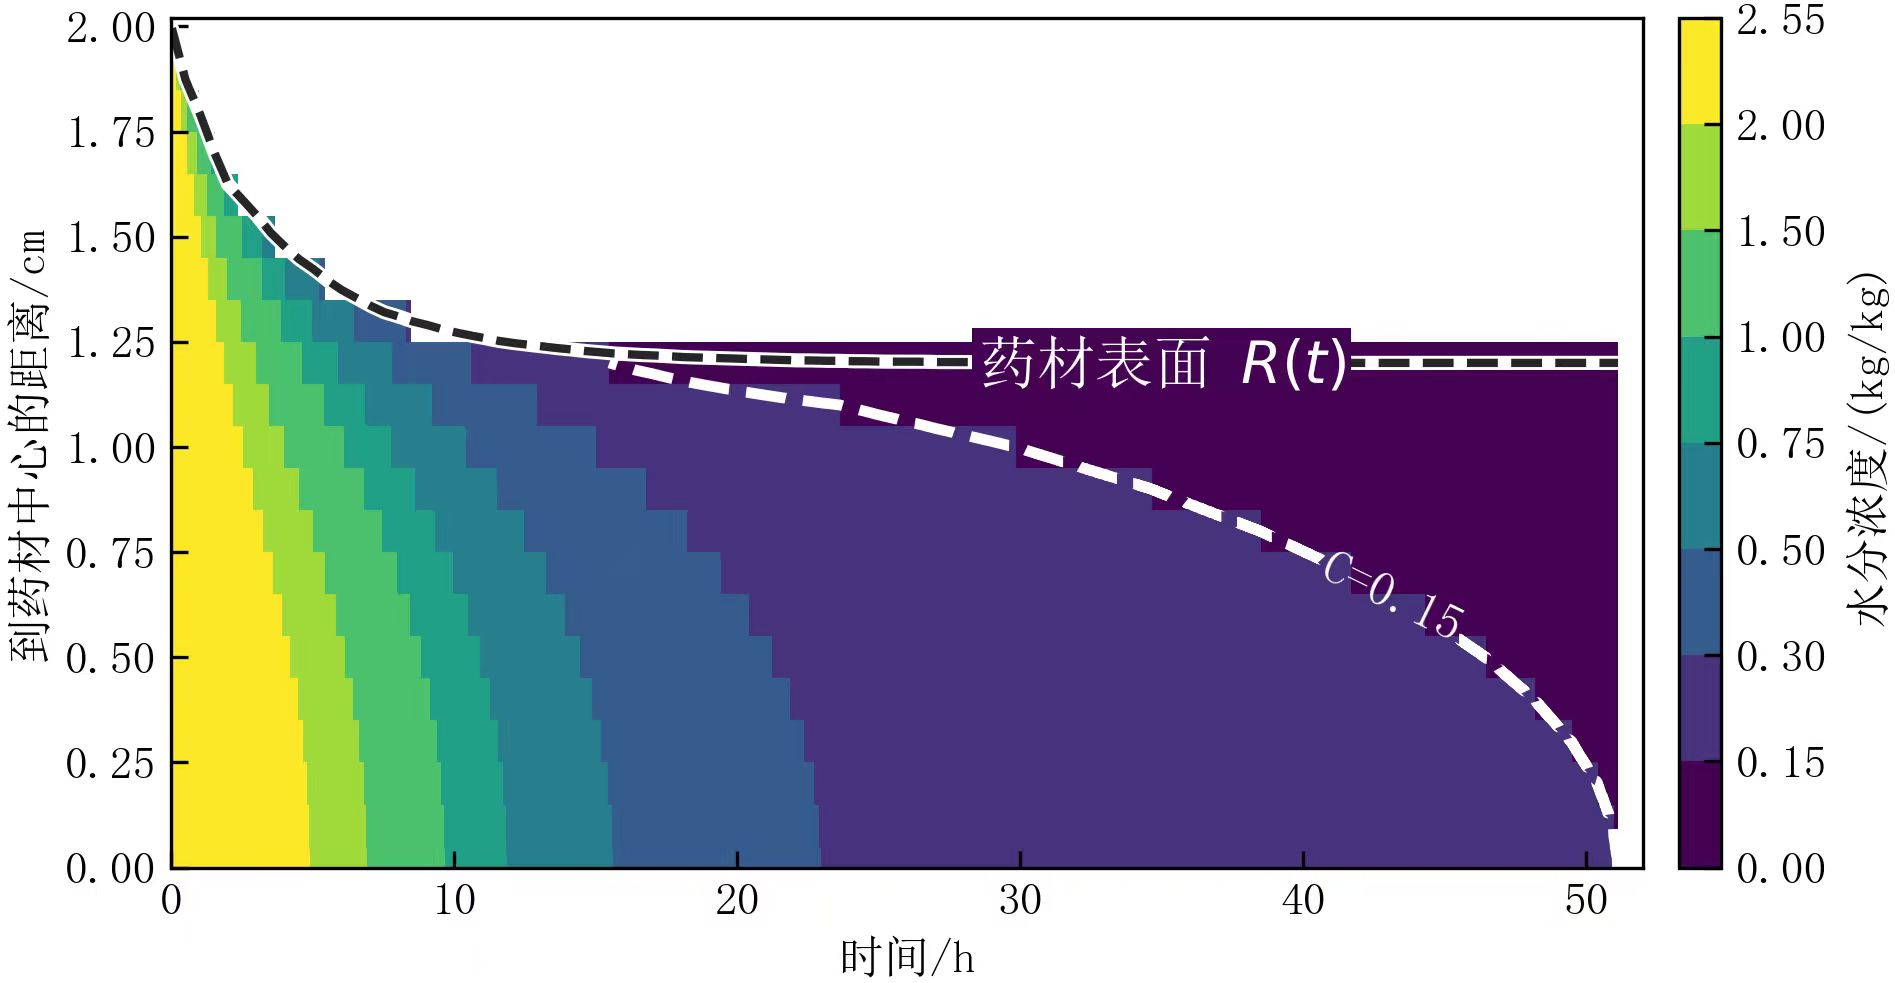
\includegraphics[width=0.8\textwidth]{Figures/q4_spatiotemporal.jpg}
    \caption{考虑尺寸变化时药材内部水分浓度的时空演化}
    \label{fig:q4_spatiotemporal}
\end{figure}

\begin{figure}[htbp]
    \centering
    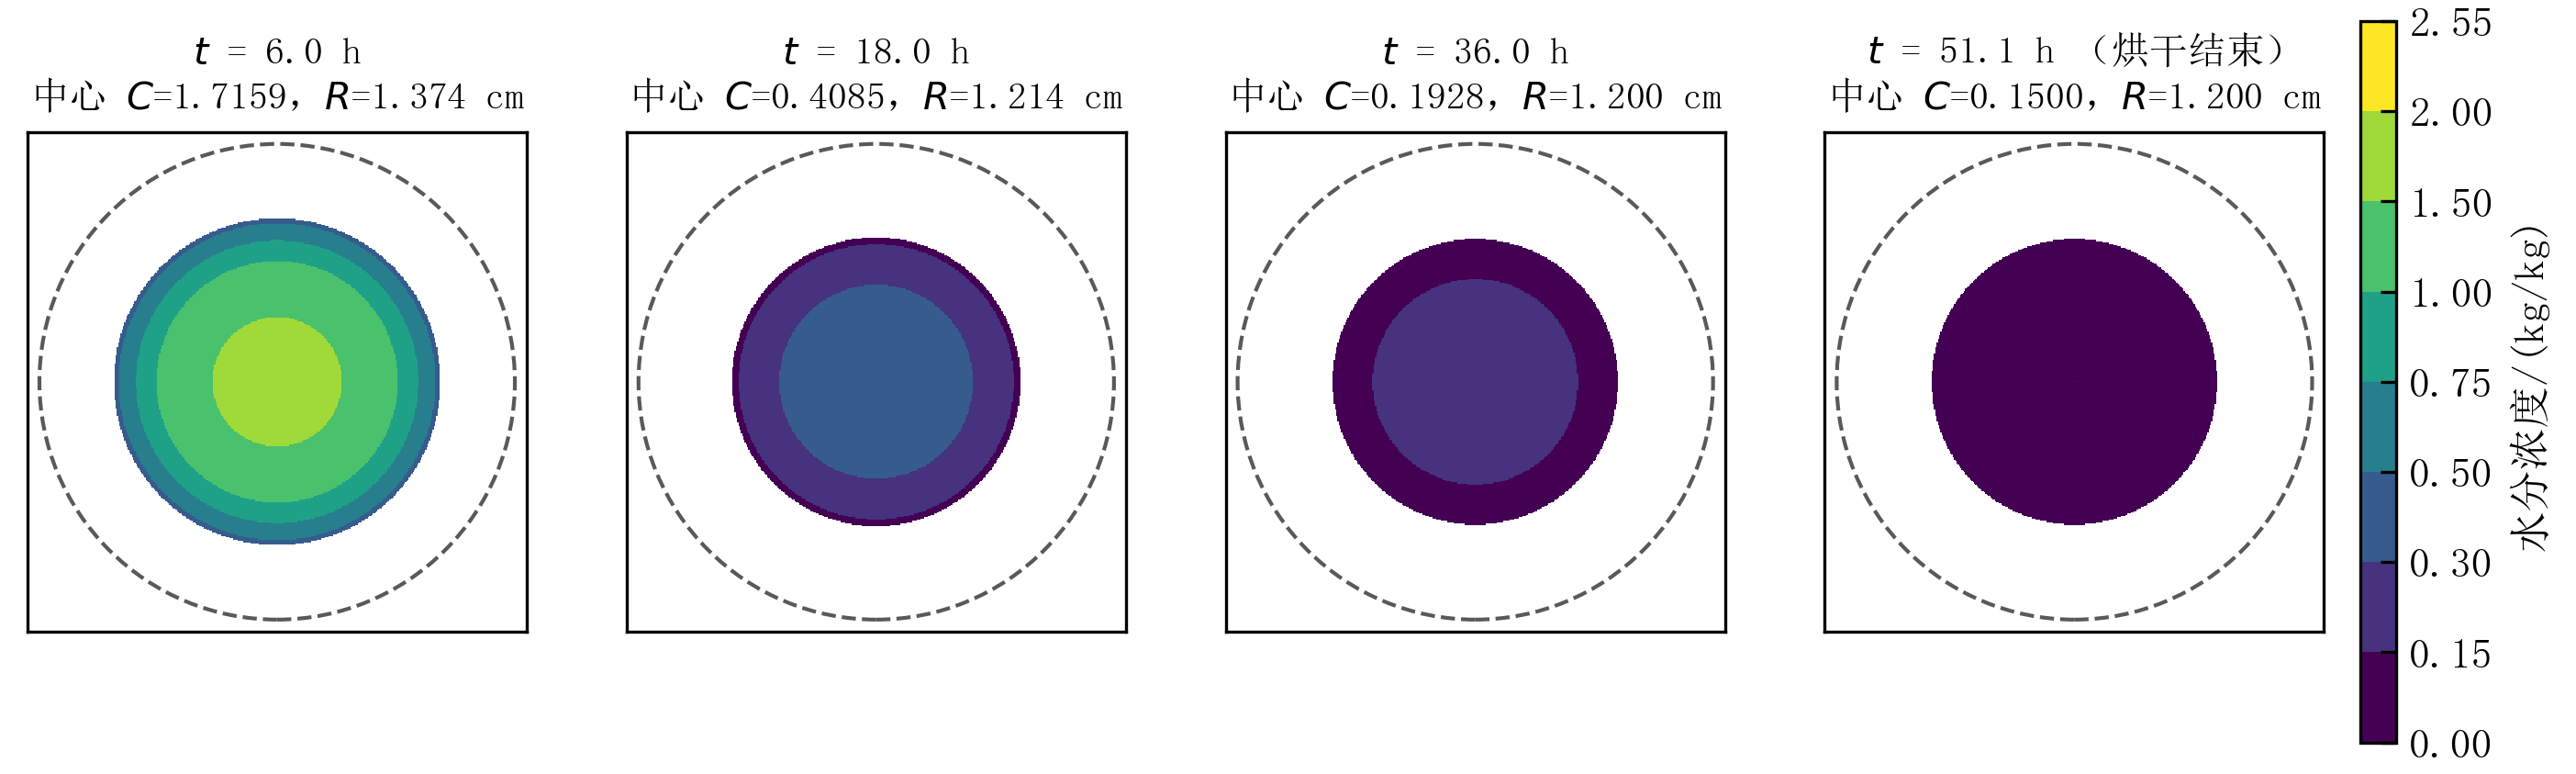
\includegraphics[width=1\textwidth]{Figures/q4_heng.png}
    \caption{横截面水分含量示意图}
    \label{fig:q4_heng}
\end{figure}

由图~\ref{fig:q4_spatiotemporal} 可见，干燥初期水分浓度梯度主要集中在表层，中心区域仍保持较高的水分浓度；随着烘干进行，水分浓度由表及里逐渐降低，高浓度区域不断向内收缩。图中白色点划线所示的药材表面 \(R(t)\) 在头 \(24\,\mathrm{h}\) 内快速下降，与附件2的实测收缩规律一致；此后趋于稳定，说明尺寸变化主要发生在干燥前期。到了干燥后期，中心区域的水分浓度逐渐逼近 \(0.15\,\mathrm{kg/kg}\) 的终止线，最终在 \(51.12\,\mathrm{h}\) 时首次满足烘干要求。

结合表~\ref{tab:moist4} 与图~\ref{fig:q4_spatiotemporal} 可以看出，整个烘干过程可以划分为两个阶段。前期，药材整体含水率较高，扩散系数相对较大，且半径快速收缩使扩散路径同步缩短，二者共同作用使水分迁移受到明显的几何加速；后期，药材半径趋于稳定，尺寸变化对扩散过程的影响逐渐减弱，此时由低含水率导致的扩散系数塌陷重新成为控制干燥速率的主要因素，中心区域的水分需要经过较长时间才能降至 \(0.15\,\mathrm{kg/kg}\) 以下。

图~\ref{fig:q4_heng} 可以看出前6h尺寸的收缩是剧烈的，但是之后的40h，尺寸的收缩就很微小。对比图~\ref{fig:q3_heng} ,也可以看出考虑尺寸变化后干壳效应没有那么明显。

因此，问题四所描述的干燥过程可以概括为 \textbf{前期：快速失水 + 快速收缩 + 扩散加速} , \textbf{后期：收缩趋缓 + 扩散系数降低 + 内部扩散控制}。
与问题三相比，考虑尺寸变化后的模型能够更加真实地反映药材实际烘干过程。

\subsubsection{模型检验与敏感性分析}

为验证问题四模型及数值结果的可靠性，本文分别从守恒性、空间网格敏感性等方面进行检验。

\paragraph{（1）水分守恒检验}

由于问题四采用物质坐标 \(\xi\)，药材实际体积随 \(R(t)^2\) 变化，因此水分守恒检验不能直接采用固定半径模型中的积分形式。对于任意物质区间 \(\xi_1\le\xi\le\xi_2\)，其干物质质量保持不变，因此水分守恒关系可以写为
\begin{equation}
\frac{\mathrm d}{\mathrm d\tau}
\left[
R^2
\int_{\xi_1}^{\xi_2}
2\xi C\,\mathrm d\xi
\right]
=
\frac{2}{R}
\left[
\xi D
\frac{\partial C}{\partial\xi}
\right]_{\xi_1}^{\xi_2}.
\label{eq:masscheck4}
\end{equation}
式~\eqref{eq:masscheck4} 中的 \(R^2\) 项十分重要，它反映了药材实际横截面积随收缩发生变化。计算得到水分守恒残差为 \(1.1\times10^{-15}\)，能量守恒残差为 \(1.2\times10^{-12}\)，均远小于输出精度 \(10^{-4}\)，说明模型具有良好的守恒性质。

\paragraph{（2）退化检验}

为了验证动边界坐标变换是否正确，将药材半径固定为 \(R(t)=2.000\,\mathrm{cm}\)，此时问题四的动态区域应退化为问题三中的固定区域模型。分别采用固定物理坐标 \(r\) 和变换后的物质坐标 \(\xi\) 进行计算，两种方法得到的烘干时间分别为
\[
t_{\mathrm{end}}^{(r)}
=
130.58\,\mathrm{h},
\qquad
t_{\mathrm{end}}^{(\xi)}
=
130.58\,\mathrm{h},
\]
二者完全一致，说明 \(\xi=r/R(t)\) 的坐标变换以及固定域控制方程推导正确，没有引入虚假的对流项或漏掉因子 \(R(t)\)。

\paragraph{（3）空间网格敏感性分析}

由于问题四中存在低含水率区域，仍需要检验空间网格对最终烘干时间的影响。分别采用不同空间区间数进行计算，结果如下。

\begin{figure}[htbp]
    \centering
    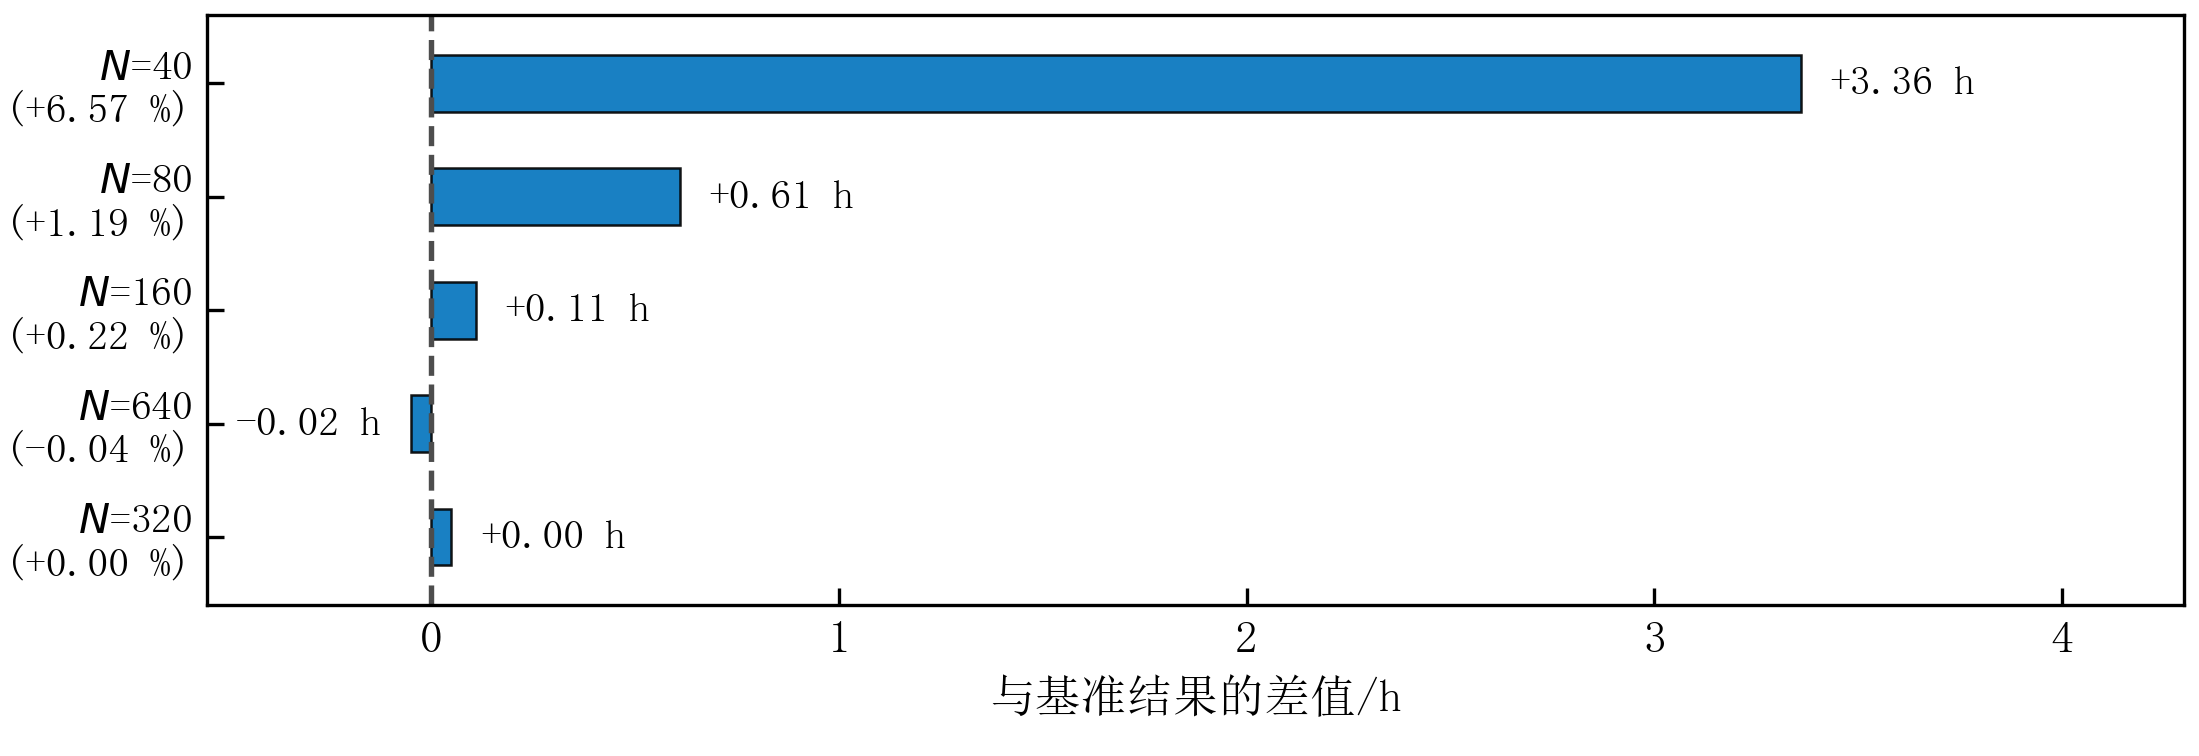
\includegraphics[width=1\textwidth]{Figures/q4_N.png}
    \caption{空间网格敏感性检验图}
    \label{fig:q4_N}
\end{figure}

由图~\ref{fig:q4_N} 可以观察到，随着网格逐渐加密，计算得到的烘干时间趋于稳定。当 \(N\) 达到 \(320\) 后，继续增加网格数量对最终烘干时间的影响已经较小，因此本文取 \(N=320\) 作为最终计算网格。

与问题三相比，问题四的网格敏感性明显降低。尺寸的收缩可以削弱干壳效应，我们不需要特别精细的网格用来分辨问题三中的干壳。








\section{模型评价}

\subsection{优点}
\begin{enumerate}
  \setlength{\itemsep}{0pt}
  \setlength{\parskip}{0pt}
  \setlength{\topsep}{2pt}
  \setlength{\partopsep}{0pt}
  \item 采用 Fick 扩散定律和 Fourier 热传导定律建模，模型具有物理意义。
  \item 考虑了烘干过程中尺寸的变化以及干壳效应，符合真实情形。
  \item 求解时采用有限体积法 + Crank--Nicolson 格式 + Picard 收敛，求解精度较好。
\end{enumerate}

\subsection{缺点}
\begin{enumerate}
  \setlength{\itemsep}{0pt}
  \setlength{\parskip}{0pt}
  \setlength{\topsep}{2pt}
  \setlength{\partopsep}{0pt}
  \item 模型未考虑汽化潜热，实际该项对结果影响很大。
  \item 由于干壳效应，模型对精度的要求比较高，计算量较大。
\end{enumerate}

\section*{AI工具使用情况说明}

本队在竞赛过程中使用了 DeepSeek DS 4.1 Flash、ChatGPT GPT-5.6 和 Agent 工作流等 AI 工具。

DeepSeek DS 4.1 Flash 主要用于模型假设与符号定义检查、代码调试和报错排查：在模型假设阶段，借助其检查假设是否遗漏、符号定义是否准确，在编程求解阶段，借助其辅助分析报错原因和提出修改思路，最终代码由本队结合模型公式与程序流程进行核验。
ChatGPT GPT-5.6 主要用于文献检索前期的关键词生成、结果分析初步讨论以及论文语言润色和结构优化：在文献检索阶段，团队在其生成关键词基础上进行补充、删除和调整，并在学术数据库中人工检索和筛选，在结果分析阶段，仅将其作为讨论参考，团队结合原始数据、模型参数和检验结果重新判断，在论文撰写阶段，用于语言表达、结构调整和学术化表述优化。
Agent 工作流主要用于论文初稿检查、结构分析和多步自动执行辅助：团队利用其对论文整体结构、章节衔接和表达逻辑进行初步检查，相关建议经人工核对后取舍，不直接作为论文结论。使用方式包括网页对话框交互、上传文件或数据对话以及 AI 智能体工作流，未使用代码编辑器内嵌 AI。
所有 AI 输出内容均经人工审查与核实，核心建模与分析由本队主导完成。

本队 AI 工具使用情况真实完整，无隐瞒、无虚假陈述，符合《全国大学生数学建模竞赛章程》《全国大学生数学建模竞赛竞赛规则》以及竞赛组委会关于 AI 工具使用的相关规定和学术诚信要求。如有不实，本队愿承担相应责任。


\begin{thebibliography}{99}
\bibitem{liu2022}
刘鹤, 焦俊华, 田友, 等. 马铃薯片热风干燥特性及收缩动力学模型[J].
食品工业科技, 2022, 43(11): 58--64.

\bibitem{Garcia2018}
J. García del Valle and J. Sierra Pallares,
``Analytical solution for the coupled heat and mass transfer formulation of one-dimensional drying kinetics,''
\textit{Journal of Food Engineering},
vol. 230, pp. 99--113, 2018.
doi: 10.1016/j.jfoodeng.2018.02.029.

\bibitem{LemusMondaca2013}
R. A. Lemus-Mondaca, C. E. Zambra, A. Vega-Gálvez, and N. O. Moraga,
``Coupled 3D heat and mass transfer model for numerical analysis of drying process in papaya slices,''
\textit{Journal of Food Engineering},
vol. 116, no. 1, pp. 109--117, 2013.
doi: 10.1016/j.jfoodeng.2012.10.050.

\bibitem{Ali2026}
I. Ali,
``Two-dimensional numerical modeling and simulation of heat and moisture transfer during drying,''
\textit{AIMS Mathematics},
vol. 11, no. 3, pp. 8762--8791, 2026.
doi: 10.3934/math.2026360.

\bibitem{dasilva2014}
da Silva W P, e Silva C M D P S, Gama F J A. Estimation of thermo-physical
properties of products with cylindrical shape during drying: The coupling
between mass and heat[J]. Journal of Food Engineering, 2014, 141: 65--73.

\bibitem{adrover2019}
Adrover A, Brasiello A. A moving boundary model for food isothermal drying
and shrinkage: One-dimensional versus two-dimensional approaches[J].
Journal of Food Process Engineering, 2019, 42(6): e13178.

\end{thebibliography}

	
	
	


	
	% ========== 附录 ==========
	\clearpage
	\appendix
	\section*{附录}
	\addcontentsline{toc}{section}{附录}
\subsection*{附录一：支撑材料结构}
\begin{table}[htbp]
    \centering
    \renewcommand{\arraystretch}{1.35}
    \begin{tabularx}{\textwidth}{|c|c|X|}
        \hline
        \textbf{支撑材料} & \textbf{文件名} & \textbf{内容说明} \\
        \hline
        \multirow{9}{*}{代码} & plot\_q1.py & 绘制问题1相关图表的代码 \\
        \cline{2-3}
         & plot\_q4.py & 绘制问题4相关图表的代码 \\
        \cline{2-3}
         & plot\_q23.py & 绘制问题2和问题3相关图表的代码 \\
        \cline{2-3}
         & q1.py & 问题1的求解代码 \\
        \cline{2-3}
         & q2.py & 问题2的求解代码 \\
        \cline{2-3}
         & q3.py & 问题3的求解代码 \\
        \cline{2-3}
         & q4.py & 问题4的求解代码 \\
        \cline{2-3}
         & sensitivity\_q4.py & 问题4灵敏度分析的代码 \\
        \cline{2-3}
         & sensitivity\_q123.py & 问题1、2、3灵敏度分析的代码 \\
        \hline
        \multirow{5}{*}{附件} & result1.xlsx & 问题1的结果数据表 \\
        \cline{2-3}
         & result2.xlsx & 问题2的结果数据表 \\
        \cline{2-3}
         & result3.xlsx & 问题3的结果数据表 \\
        \cline{2-3}
         & result4.xlsx & 问题4的结果数据表 \\
        \hline
         & AI工具使用详情.pdf & 竞赛过程中AI工具使用情况说明 \\
        \hline
    \end{tabularx}
\end{table}

\subsection*{附录二：核心程序代码}
由于篇幅限制，附录中仅展示四个问题求解的核心代码，其余作图以及敏感性分析使用的代码都在支撑材料中展示。
\subsubsection*{1. 问题一求解代码}

\begin{lstlisting}
import sys, math, openpyxl

RHO, CP, K = 820.0, 2600.0, 0.36      
H, HM = 25.0, 8.0e-7                  
X0, T0 = 2.55, 28.0                   
R, N = 0.02, 80                       
RHO_D = RHO / (1 + X0)                
LV = 2.43e6 if '--latent' in sys.argv else 0.0
AIR, OUT = '附件/附件1.xlsx', '附件/附件3/result1.xlsx'
DISTS = [round(0.1 * i, 1) for i in range(21)]
THETA = 0.5                           

def D_of(X):
    return 7e-9 * math.exp(-0.89 / X) if X > 1e-9 else 0.0
def setup(n):
    global N, dr, V, A
    N, dr = n, R / n
    V, A = [], []                     
    for i in range(n + 1):
        lo = max(i * dr - dr / 2, 0.0)
        hi = R if i == n else i * dr + dr / 2
        V.append((hi * hi - lo * lo) / 2)
        A.append(min(i * dr + dr / 2, R))
def air_at(t, col):
    i = min(int(t // 60), len(AIRDATA) - 2)
    f = (t - AIRDATA[i][0]) / (AIRDATA[i + 1][0] - AIRDATA[i][0])
    return AIRDATA[i][col] * (1 - f) + AIRDATA[i + 1][col] * f
def thomas(a, b, c, d):
    n = len(d)
    cp, dp = [0.0] * n, [0.0] * n
    cp[0], dp[0] = c[0] / b[0], d[0] / b[0]
    for i in range(1, n):
        m = b[i] - a[i] * cp[i - 1]
        dp[i] = (d[i] - a[i] * dp[i - 1]) / m
        if i < n - 1:
            cp[i] = c[i] / m
    x = [0.0] * n
    x[-1] = dp[-1]
    for i in range(n - 2, -1, -1):
        x[i] = dp[i] - cp[i] * x[i + 1]
    return x
def advance(u, u_inf, gface, bc, h, src=None):
    n = N + 1
    d = [V[i] / h * u[i] for i in range(n)]
    Rr = [0.0] * n                                    
    Rr[0] = gface[0] * (u[1] - u[0])
    for i in range(1, N):
        Rr[i] = gface[i] * (u[i + 1] - u[i]) - gface[i - 1] * (u[i] - u[i - 1])
    Rr[N] = A[N] * bc * (u_inf - u[N]) - gface[N - 1] * (u[N] - u[N - 1])
    for i in range(n):
        d[i] += (1 - THETA) * Rr[i] + (src[i] if src else 0.0)
    a, b, c = [0.0] * n, [0.0] * n, [0.0] * n
    b[0], c[0] = V[0] / h + THETA * gface[0], -THETA * gface[0]
    for i in range(1, N):
        a[i] = -THETA * gface[i - 1]
        b[i] = V[i] / h + THETA * (gface[i - 1] + gface[i])
        c[i] = -THETA * gface[i]
    a[N] = -THETA * gface[N - 1]
    b[N] = V[N] / h + THETA * (gface[N - 1] + A[N] * bc)
    d[N] += THETA * A[N] * bc * u_inf
    return thomas(a, b, c, d)
def harm(a, b):                                       
    return 2 * a * b / (a + b) if a + b > 0 else 0.0
def solve(dt=1.0, tmax=1800.0, nsub=1):
    X, T = [X0] * (N + 1), [T0] * (N + 1)
    snaps, loss, heat = [], 0.0, 0.0
    h = dt / nsub
    for step in range(1, int(round(tmax / dt)) + 1):
        for sub in range(nsub):
            t = (step - 1) * dt + sub * h + h / 2     
            x_inf, t_inf = air_at(t, 2), air_at(t, 1)
            X_prev = X[:]

            for _ in range(3):                        
                D = [D_of(v) for v in X]
                gf = [A[i] * harm(D[i], D[i + 1]) / dr for i in range(N)]
                Xn = advance(X_prev, x_inf, gf, HM, h)
                if max(abs(Xn[i] - X[i]) for i in range(N + 1)) < 1e-13:
                    X = Xn
                    break
                X = Xn
            loss += h * A[N] * HM * (THETA * (X[N] - x_inf)
                                     + (1 - THETA) * (X_prev[N] - x_inf))

            gf = [A[i] * (K / (RHO * CP)) / dr for i in range(N)]
            src = None
            if LV > 0:                                
                q = RHO_D * LV / (RHO * CP) / h
                src = [q * V[i] * (X[i] - X_prev[i]) for i in range(N + 1)]
            T_prev = T[:]
            T = advance(T, t_inf, gf, H / (RHO * CP), h, src)
            heat += h * A[N] * (H / (RHO * CP)) * (
                THETA * (t_inf - T[N]) + (1 - THETA) * (t_inf - T_prev[N]))
        snaps.append((step * dt, T[:], X[:]))
    return snaps, loss, heat
def write_xlsx(snaps, stride):
    wb = openpyxl.load_workbook(OUT)
    for name, k in (('温度', 0), ('水分浓度', 1)):
        ws = wb[name]
        ws.cell(1, 1, '时间\\到药材中心的距离')
        for j, d0 in enumerate(DISTS):
            ws.cell(1, j + 2, d0)
        for i, s in enumerate(snaps):
            ws.cell(i + 2, 1, int(s[0]))
            for j in range(21):
                cell = ws.cell(i + 2, j + 2, round(s[k + 1][j * stride], 4))
                cell.number_format = '0.0000'
    wb.save(OUT)

if __name__ == '__main__':
    AIRDATA = [(r[0], r[1], r[2]) for r in openpyxl.load_workbook(
        AIR, data_only=True).active.iter_rows(min_row=2, values_only=True)]
    N0 = N                                            
    stride = N // 20                                  
    setup(N)
    snaps, loss, heat = solve()
    T, X = snaps[-1][1], snaps[-1][2]
    outT = [T[j * stride] for j in range(21)]
    outX = [X[j * stride] for j in range(21)]
    m_lost = sum(V[i] * (X0 - X[i]) for i in range(N + 1))
    assert abs(m_lost - loss) / m_lost < 1e-9, (m_lost, loss)
    dv = sum(V[i] * (T[i] - T0) for i in range(N + 1))
    if LV > 0:
        dv += sum(RHO_D * LV / (RHO * CP) * V[i] * (X0 - X[i]) for i in range(N + 1))
    assert abs(dv - heat) / abs(heat) < 1e-9, (dv, heat)
    s2, _, _ = solve(dt=1.0, nsub=4)
    e_dt = max(max(abs(p - q) for p, q in zip(T, s2[-1][1])),
               max(abs(p - q) for p, q in zip(X, s2[-1][2])))
    setup(2 * N)
    s3, _, _ = solve()
    e_dr = max(max(abs(outT[j] - s3[-1][1][j * 2 * stride]) for j in range(21)),
               max(abs(outX[j] - s3[-1][2][j * 2 * stride]) for j in range(21)))
    setup(N0)
    assert e_dt < 5e-5 and e_dr < 2e-4, (e_dt, e_dr)
    print('自检通过: 水分守恒 %.1e, 能量守恒 %.1e, dt 减半 %.1e, dr 减半 %.1e (0.025cm), 潜热项 %s'
          % (abs(m_lost - loss) / m_lost, abs(dv - heat) / abs(heat),
             e_dt, e_dr, '开' if LV else '关'))
    xbar = sum(V[i] * X[i] for i in range(N + 1)) / sum(V)
    print('1800 s 平均含水率 %.4f (ΔX=%.4f); 半径比 预测 %.4f / 附件2 实测 %.4f'
          % (xbar, X0 - xbar, math.sqrt((1 + xbar) / (1 + X0)), 1.873 / 2.0))
    idx = {int(s[0]): (s[1], s[2]) for s in snaps}
    dist = (0, .5, 1, 1.5, 2)
    for title, k, unit in (('表 1 药材温度', 0, 'degC'), ('表 2 水分浓度', 1, 'kg/kg')):
        print('\n%s (%s)' % (title, unit))
        print('时间/s   ' + ''.join('r=%-7.1f' % d for d in dist))
        for t in (100, 300, 600, 900, 1200, 1500, 1800):
            print('%-9d' % t + ''.join('%9.4f' % idx[t][k][int(d * 10) * stride]
                                       for d in dist))
    if '--no-write' not in sys.argv:
        write_xlsx(snaps, stride)
        print('\n已写入 %s (%d 行 x 22 列)' % (OUT, len(snaps) + 1))
\end{lstlisting}
\subsubsection*{2. 问题二求解代码}
\begin{lstlisting}
import sys
import math
import openpyxl
from q1 import thomas

R, N = 0.02, 80                       
H, HM = 25.0, 8.0e-7                  
X0, T0 = 2.55, 28.0                   
TSTAR = 7200.0                        
T_PLAT, X_PLAT = 50.0, 0.050          
THETA = 0.5                           
AIR, OUT = '附件/附件1.xlsx', '附件/附件3/result2.xlsx'
DISTS = [round(0.1 * i, 1) for i in range(21)]

def rho(C):
    return 650 + 128 * C
def cp(C):
    return 1450 + 2736 * C / (C + 1)
def kof(C):
    return 0.21 + 0.38 * C / (C + 1)
def Dof(C, Tc):
    if C < 1e-6:
        return 0.0
    return 2.4e-3 * math.exp(-0.45 / C) * math.exp(-3850 / (Tc + 273.15))
def env(t, airdata):
    if t >= TSTAR:
        return T_PLAT, X_PLAT
    i = min(int(t // 60), len(airdata) - 2)
    f = (t - airdata[i][0]) / (airdata[i + 1][0] - airdata[i][0])
    return (airdata[i][1] * (1 - f) + airdata[i + 1][1] * f,
            airdata[i][2] * (1 - f) + airdata[i + 1][2] * f)
def setup(n):
    global N, dr, V, A
    N, dr = n, R / n
    V, A = [], []
    for i in range(n + 1):
        lo = max(i * dr - dr / 2, 0.0)
        hi = R if i == n else i * dr + dr / 2
        V.append((hi * hi - lo * lo) / 2)
        A.append(min(i * dr + dr / 2, R))
def harm(a, b):
    return 2 * a * b / (a + b) if a + b > 0 else 0.0
def advance(u, u_inf, gface, bc, h, cap):
    n = N + 1
    Rr = [0.0] * n
    Rr[0] = gface[0] * (u[1] - u[0])
    for i in range(1, N):
        Rr[i] = gface[i] * (u[i + 1] - u[i]) - gface[i - 1] * (u[i] - u[i - 1])
    Rr[N] = A[N] * bc * (u_inf - u[N]) - gface[N - 1] * (u[N] - u[N - 1])
    d = [cap[i] * V[i] / h * u[i] + (1 - THETA) * Rr[i] for i in range(n)]
    a = [0.0] * n
    b = [0.0] * n
    c = [0.0] * n
    b[0] = cap[0] * V[0] / h + THETA * gface[0]
    c[0] = -THETA * gface[0]
    for i in range(1, N):
        a[i] = -THETA * gface[i - 1]
        b[i] = cap[i] * V[i] / h + THETA * (gface[i - 1] + gface[i])
        c[i] = -THETA * gface[i]
    a[N] = -THETA * gface[N - 1]
    b[N] = cap[N] * V[N] / h + THETA * (gface[N - 1] + A[N] * bc)
    d[N] += THETA * A[N] * bc * u_inf
    return thomas(a, b, c, d)
def solve(dt=1.0, tmax=10800.0, nsub=1, airdata=None, keep=1, stop=None):
    C = [X0] * (N + 1)
    T = [T0] * (N + 1)
    snaps, loss, heat, store = [], 0.0, 0.0, 0.0
    h = dt / nsub
    for step in range(1, int(round(tmax / dt)) + 1):
        for sub in range(nsub):
            t = (step - 1) * dt + sub * h + h / 2
            t_inf, x_inf = env(t, airdata)
            C_old, T_old = C[:], T[:]
            cap = [1.0] * (N + 1)
            for _ in range(4):                    
                D = [Dof(C[i], T[i]) for i in range(N + 1)]
                gfC = [A[i] * harm(D[i], D[i + 1]) / dr for i in range(N)]
                Cn = advance(C_old, x_inf, gfC, HM, h, [1.0] * (N + 1))
                kk = [kof(Cn[i]) for i in range(N + 1)]
                gfT = [A[i] * harm(kk[i], kk[i + 1]) / dr for i in range(N)]
                cap = [rho(Cn[i]) * cp(Cn[i]) for i in range(N + 1)]
                Tn = advance(T_old, t_inf, gfT, H, h, cap)
                conv = (max(abs(Cn[i] - C[i]) for i in range(N + 1)) < 1e-11
                        and max(abs(Tn[i] - T[i]) for i in range(N + 1)) < 1e-9)
                C, T = Cn, Tn
                if conv:
                    break
            loss += h * A[N] * HM * (THETA * (C[N] - x_inf)
                                     + (1 - THETA) * (C_old[N] - x_inf))
            heat += h * A[N] * H * (THETA * (t_inf - T[N])
                                    + (1 - THETA) * (t_inf - T_old[N]))
            store += sum(cap[i] * V[i] * (T[i] - T_old[i]) for i in range(N + 1))
        if step % keep == 0:
            snaps.append((step * dt, T[:], C[:]))
            if stop is not None and max(C) <= stop:
                break
    return snaps, loss, heat, store
def write_xlsx(snaps, stride):
    wb = openpyxl.load_workbook(OUT)
    for name, k in (('温度', 1), ('水分浓度', 2)):
        ws = wb[name]
        ws.cell(1, 1, '时间\\到药材中心的距离')
        for j, d0 in enumerate(DISTS):
            ws.cell(1, j + 2, d0)
        for i, s in enumerate(snaps):
            ws.cell(i + 2, 1, int(s[0]))
            for j in range(21):
                cell = ws.cell(i + 2, j + 2, round(s[k][j * stride], 4))
                cell.number_format = '0.0000'
    wb.save(OUT)

if __name__ == '__main__':
    AIRDATA = [(r[0], r[1], r[2]) for r in openpyxl.load_workbook(
        AIR, data_only=True).active.iter_rows(min_row=2, values_only=True)]
    N0 = N
    stride = N0 // 20

    setup(N0)
    snaps, loss, heat, store = solve(airdata=AIRDATA)
    T, C = snaps[-1][1], snaps[-1][2]
    outT = [T[j * stride] for j in range(21)]
    outC = [C[j * stride] for j in range(21)]

    if '--no-check' not in sys.argv:
        m_lost = sum(V[i] * (X0 - C[i]) for i in range(N + 1))
        assert abs(m_lost - loss) / m_lost < 1e-9, (m_lost, loss)
        assert abs(store - heat) / abs(heat) < 1e-9, (store, heat)
        s2, _, _, _ = solve(dt=1.0, nsub=2, tmax=3600.0, airdata=AIRDATA)
        e_dt = max(max(abs(p - q) for p, q in zip(snaps[3599][1], s2[-1][1])),
                   max(abs(p - q) for p, q in zip(snaps[3599][2], s2[-1][2])))
        setup(2 * N0)
        s3, _, _, _ = solve(tmax=3600.0, airdata=AIRDATA)
        e_dr = max(
            max(abs(snaps[3599][1][j * stride] - s3[-1][1][j * 2 * stride])
                for j in range(21)),
            max(abs(snaps[3599][2][j * stride] - s3[-1][2][j * 2 * stride])
                for j in range(21)))
        setup(N0)
        assert e_dt < 5e-5 and e_dr < 5e-4, (e_dt, e_dr)
        print('自检通过: 水分守恒 %.1e, 能量守恒 %.1e, dt 减半 %.1e, dr 减半 %.1e'
              % (abs(m_lost - loss) / m_lost, abs(store - heat) / abs(heat), e_dt, e_dr))
    idx = {int(s[0]): s for s in snaps}
    dist = (0, .5, 1, 1.5, 2)
    for title, k, unit in (('表 3 药材温度', 1, 'degC'),
                           ('表 4 水分浓度', 2, 'kg/kg')):
        print('\n%s (%s)' % (title, unit))
        print('时间/h   ' + ''.join('r=%-7.1f' % d for d in dist))
        for hh in (0.5, 1.0, 1.5, 2.0, 2.5, 3.0):
            print('%-9.1f' % hh + ''.join(
                '%9.4f' % idx[int(hh * 3600)][k][int(d * 10) * stride]
                for d in dist))

    if '--no-write' not in sys.argv:
        write_xlsx(snaps, stride)
        print('\n已写入 %s (%d 行 x 22 列)' % (OUT, len(snaps) + 1))
\end{lstlisting}

\subsubsection*{3. 问题三求解代码}

\begin{lstlisting}
import sys
import openpyxl
import q2 as Q2

CRIT = 0.15                     
AIR = '附件/附件1.xlsx'
OUT = '附件/附件3/result3.xlsx'
DISTS = [round(0.1 * i, 1) for i in range(21)]

def airdata():
    return [(r[0], r[1], r[2]) for r in openpyxl.load_workbook(
        AIR, data_only=True).active.iter_rows(min_row=2, values_only=True)]
def run(n, dt, tmax, data, keep=1, stop=None):
    Q2.setup(n)
    return Q2.solve(dt=dt, tmax=tmax, airdata=data, keep=keep, stop=stop)
def write_xlsx(snaps, stride):
    wb = openpyxl.load_workbook(OUT)
    wb.remove(wb['Sheet1'])                    
    ws = wb.create_sheet('Sheet1', 0)
    ws.cell(1, 1, '时间\\到药材中心的距离')
    for j, d0 in enumerate(DISTS):
        ws.cell(1, j + 2, d0)
    for i, s in enumerate(snaps):
        ws.cell(i + 2, 1, int(s[0]))
        for j in range(21):
            cell = ws.cell(i + 2, j + 2, round(s[2][j * stride], 4))
            cell.number_format = '0.0000'
    try:
        wb.save(OUT)
        return len(snaps), OUT
    except PermissionError:            
        alt = OUT.replace('.xlsx', '_修正.xlsx')
        wb.save(alt)
        return len(snaps), alt

if __name__ == '__main__':
    data = airdata()
    N0, DT, TMAX = 320, 10.0, 6.0e5         
    stride = N0 // 20
    snaps, loss, heat, store = run(N0, DT, TMAX, data, keep=6, stop=CRIT)
    assert max(snaps[-1][2]) <= CRIT, '未在 TMAX 内达标，请加大 TMAX'
    t_end = snaps[-1][0]
    idx = {int(s[0]): s for s in snaps}
    vol = sum(Q2.V)
    t_surf = next(s[0] for s in snaps if s[2][Q2.N] <= CRIT)
    t_avg = next(s[0] for s in snaps
                 if sum(Q2.V[i] * s[2][i] for i in range(Q2.N + 1)) / vol <= CRIT)
    cend = snaps[-1][2]
    m_lost = sum(Q2.V[i] * (Q2.X0 - cend[i]) for i in range(Q2.N + 1))
    assert abs(m_lost - loss) / m_lost < 1e-9, (m_lost, loss)
    assert min(cend) > 0.0 and all(
        max(snaps[k][2]) >= max(snaps[k + 100][2]) - 1e-9
        for k in range(0, len(snaps) - 100, 1000))
    if '--no-check' not in sys.argv:
        s2, _, _, _ = run(160, DT, TMAX, data, keep=6, stop=CRIT)
        dt_grid = abs(s2[-1][0] - t_end) / 3600
        assert dt_grid < 4.0, dt_grid
        print('自检通过: 水分守恒 %.1e, N=160 与 N=320 烘干时间差 %.2f h'
              % (abs(m_lost - loss) / m_lost, dt_grid))
    print('\n烘干结束时间: %.0f s = %.2f h = %.2f 天' % (t_end, t_end / 3600, t_end / 86400))
    print('末态: 中心 %.4f, 表面 %.4f kg/kg'
          % (idx[int(t_end)][2][0], idx[int(t_end)][2][Q2.N]))
    print('判据灵敏度: 表面 <0.15 需 %.1f h; 体积平均 <0.15 需 %.1f h; 处处 <0.15 需 %.1f h'
          % (t_surf / 3600, t_avg / 3600, t_end / 3600))
    dist = (0, .5, 1, 1.5, 2)
    print('\n表 5 药材烘干过程的水分浓度 (kg/kg)')
    print('时间/h   ' + ''.join('r=%-7.1f' % d for d in dist))
    hh = 6.0
    while hh * 3600 <= t_end:
        print('%-9.1f' % hh + ''.join(
            '%9.4f' % idx[int(hh * 3600)][2][int(d * 10) * stride] for d in dist))
        hh += 6.0
    print('%-9s' % ('%.1f(结束)' % (t_end / 3600)) + ''.join(
        '%9.4f' % idx[int(t_end)][2][int(d * 10) * stride] for d in dist))
    if '--no-write' not in sys.argv:
        nrow, path = write_xlsx(snaps, stride)
        print('\n已写入 %s (Sheet1, %d 行 x 22 列)' % (path, nrow + 1))
        if path != OUT:
            print('注意: %s 被占用（Excel 打开中），已改为写入 %s；关闭后重跑即可覆盖' % (OUT, path))

\end{lstlisting}

\subsubsection*{4. 问题四求解代码}

\begin{lstlisting}
	import sys
import math
import bisect
import openpyxl
import q2 as Q2

CRIT = 0.15                          
R_CUT = 0.5                          
N0, DT = 320, 10.0                   
AIR, RAD, OUT = '附件/附件1.xlsx', '附件/附件2.xlsx', '附件/附件3/result4.xlsx'
DISTS = [round(0.1 * i, 1) for i in range(21)]      

def D4(C, Tc):
    if C < 1e-6:
        return 0.0
    return 4.2e-4 * math.exp(-0.30 / C) * math.exp(-3850 / (Tc + 273.15))
def load_radius():
    rows = list(openpyxl.load_workbook(RAD, data_only=True)
                .active.iter_rows(min_row=2, values_only=True))
    return [(r[0], r[1] / 100.0) for r in rows]     # (s, m)
def Rof(t, rd):
    i = bisect.bisect_right(rd, (t, 1e9)) - 1
    if i < 0:
        return rd[0][1]
    if i >= len(rd) - 1:
        return rd[-1][1]
    t0, r0 = rd[i]
    t1, r1 = rd[i + 1]
    return r0 + (r1 - r0) * (t - t0) / (t1 - t0)
def solve(n=N0, dt=DT, tmax=1.5e6, keep=6, stop=CRIT, airdata=None, rd=None):
    Q2.R = 1.0                       
    Q2.setup(n)
    V, A, dxi = Q2.V, Q2.A, Q2.dr
    m = n + 1
    C, T = [Q2.X0] * m, [Q2.T0] * m
    snaps, loss, store, heat = [], 0.0, 0.0, 0.0
    for step in range(1, int(tmax / dt) + 1):
        t = (step - 1) * dt + dt / 2                 
        Rt = Rof(t, rd)
        t_inf, x_inf = Q2.env(t, airdata)
        C_old, T_old = C[:], T[:]
        cap = [1.0] * m
        for _ in range(4):                           
            D = [D4(C[i], T[i]) for i in range(m)]
            gfC = [A[i] * Q2.harm(D[i], D[i + 1]) / (dxi * Rt * Rt) for i in range(n)]
            Cn = Q2.advance(C_old, x_inf, gfC, Q2.HM / Rt, dt, [1.0] * m)
            kk = [Q2.kof(Cn[i]) for i in range(m)]
            gfT = [A[i] * Q2.harm(kk[i], kk[i + 1]) / (dxi * Rt * Rt) for i in range(n)]
            cap = [Q2.rho(Cn[i]) * Q2.cp(Cn[i]) for i in range(m)]
            Tn = Q2.advance(T_old, t_inf, gfT, Q2.H / Rt, dt, cap)
            conv = (max(abs(Cn[i] - C[i]) for i in range(m)) < 1e-11
                    and max(abs(Tn[i] - T[i]) for i in range(m)) < 1e-9)
            C, T = Cn, Tn
            if conv:
                break
        loss += dt * (Q2.HM / Rt) * (Q2.THETA * (C[n] - x_inf)
                                     + (1 - Q2.THETA) * (C_old[n] - x_inf))
        heat += dt * (Q2.H / Rt) * (Q2.THETA * (t_inf - T[n])
                                    + (1 - Q2.THETA) * (t_inf - T_old[n]))
        store += sum(cap[i] * V[i] * (T[i] - T_old[i]) for i in range(m))
        if step % keep == 0:
            snaps.append((step * dt, T[:], C[:], Rt))
            if stop is not None and max(C) <= stop:
                break
    return snaps, loss, store, heat, V
def sample(C, Rt, r, n):
    if r > Rt:
        return None
    i = r / Rt * n
    if i >= n:
        return C[n]
    lo = int(i)
    f = i - lo
    return C[lo] * (1 - f) + C[lo + 1] * f
def write_xlsx(snaps, n):
    wb = openpyxl.load_workbook(OUT)
    ws = wb['Sheet1']
    ws.cell(1, 1, '时间\\到药材中心的距离')
    for j in range(20):                              
        ws.cell(1, j + 2, DISTS[j])
    ws.cell(1, 22, '药材表面')                        
    for i, (t, T, C, Rt) in enumerate(snaps):
        ws.cell(i + 2, 1, int(t))
        for j in range(20):
            v = sample(C, Rt, DISTS[j] / 100.0, n)
            cell = ws.cell(i + 2, j + 2, None if v is None else round(v, 4))
            cell.number_format = '0.0000'
        cell = ws.cell(i + 2, 22, round(C[n], 4))
        cell.number_format = '0.0000'
    wb.save(OUT)
    return len(snaps)

if __name__ == '__main__':
    airdata = [(r[0], r[1], r[2]) for r in openpyxl.load_workbook(
        AIR, data_only=True).active.iter_rows(min_row=2, values_only=True)]
    rd = load_radius()
    assert len(rd) == 145 and abs(rd[0][1] - 0.02) < 1e-9 and rd[-1][1] < 0.0121
    snaps, loss, store, heat, V = solve(airdata=airdata, rd=rd)
    nn = Q2.N                        
    t_end, T, C, Rt = snaps[-1]
    assert max(C) <= CRIT
    m_lost = sum(V[i] * (Q2.X0 - C[i]) for i in range(len(C)))
    assert abs(m_lost - loss) / m_lost < 1e-9, (m_lost, loss)
    assert abs(store - heat) / abs(heat) < 1e-9, (store, heat)
    if '--no-check' not in sys.argv:
        d0 = Q2.Dof
        Q2.Dof = D4                                 
        Q2.R = 0.02
        Q2.setup(160)
        s3, _, _, _ = Q2.solve(dt=DT, tmax=1.5e6, airdata=airdata, keep=6, stop=CRIT)
        Q2.Dof = d0
        s2, _, _, _, _ = solve(n=160, airdata=airdata, rd=[(0, 0.02), (1e9, 0.02)])
        print('自检通过: 水分守恒 %.1e, 能量守恒 %.1e' %
              (abs(m_lost - loss) / m_lost, abs(store - heat) / abs(heat)))
        print('     退化检验(R 冻结 2cm, N=160): ξ 域 %.2f h vs r 域 %.2f h'
              % (s2[-1][0] / 3600, s3[-1][0] / 3600))
        assert abs(s2[-1][0] - s3[-1][0]) / s3[-1][0] < 0.02
    print('\n烘干结束时间: %.0f s = %.2f h = %.2f 天   (末态 R = %.3f cm)'
          % (t_end, t_end / 3600, t_end / 86400, Rt * 100))
    dist = (0, .5, 1.0, 1.5)
    idx = {int(s[0]): s for s in snaps}
    print('\n表 6 药材烘干过程的水分浓度 (kg/kg)')
    print('时间/h     ' + ''.join('r=%-8.1f' % d for d in dist) + '药材表面')
    hh = 6.0
    while hh * 3600 <= t_end:
        s = idx[int(hh * 3600)]
        row = ''
        for d in dist:
            v = sample(s[2], s[3], d / 100.0, nn)
            row += '%-10s' % ('—' if v is None else '%.4f' % v)
        print('%-11.1f' % hh + row + '%.4f' % s[2][nn])
        hh += 6.0
    row = ''
    for d in dist:
        v = sample(C, Rt, d / 100.0, nn)
        row += '%-10s' % ('—' if v is None else '%.4f' % v)
    print('%-11s' % ('%.1f(结束)' % (t_end / 3600)) + row + '%.4f' % C[nn])
    if '--no-write' not in sys.argv:
        nrow = write_xlsx(snaps, nn)
        print('\n已写入 %s (Sheet1, %d 行 x 22 列)' % (OUT, nrow + 1))
    if '--grid' in sys.argv:
        print('\n网格收敛（ξ 方向 N）:')
        for n in (160, N0, 640):
            s, _, _, _, _ = solve(n=n, airdata=airdata, rd=rd)
            print('  N=%3d  t_end = %8.2f h' % (n, s[-1][0] / 3600))
\end{lstlisting}
	
	
\end{document}